% for plotting
\documentclass[10pt]{article}
\usepackage{fullpage}
\usepackage{amsmath}    % for subequations
\usepackage{tikz}       % for generating figures with math symbols
\usepackage{graphicx}   % for figures
\usepackage{xcolor}
\usepackage{subfigure}  % for side-by-side figures

\begin{document}

\begin{figure}
  \begin{subfigure}
    \centering
    \resizebox{1.1\linewidth}{!}{% Created by tikzDevice version 0.12.3 on 2019-09-27 15:30:16
% !TEX encoding = UTF-8 Unicode
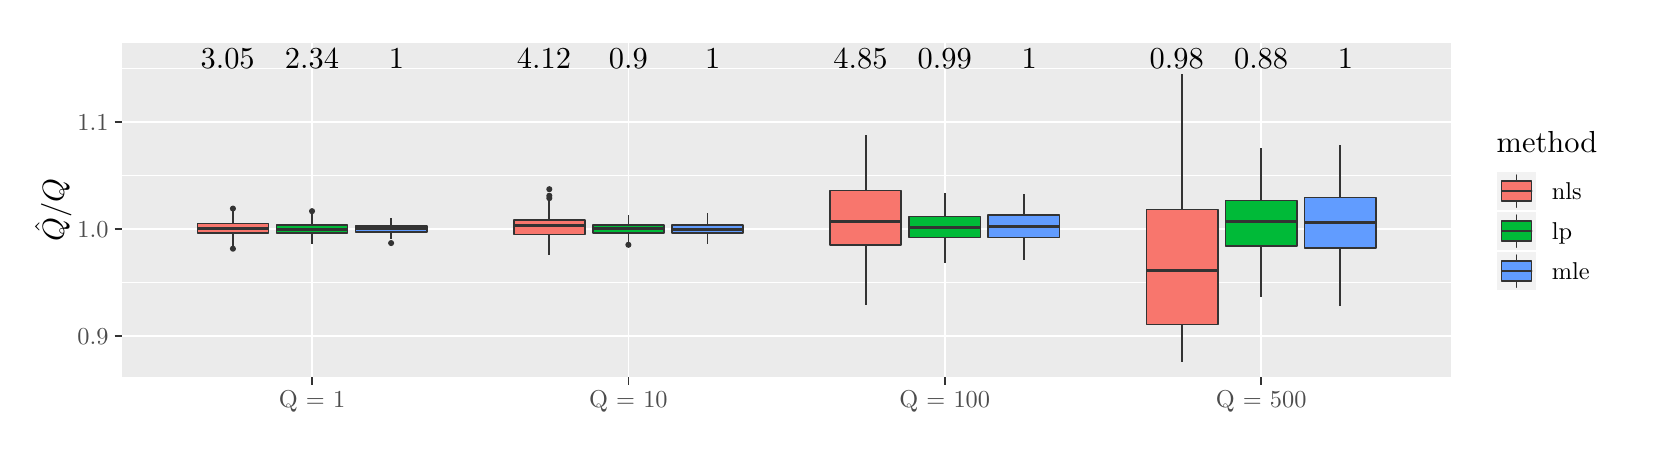
\begin{tikzpicture}[x=1pt,y=1pt]
\definecolor{fillColor}{RGB}{255,255,255}
\path[use as bounding box,fill=fillColor,fill opacity=0.00] (0,0) rectangle (578.16,144.54);
\begin{scope}
\path[clip] (  0.00,  0.00) rectangle (578.16,144.54);
\definecolor{drawColor}{RGB}{255,255,255}
\definecolor{fillColor}{RGB}{255,255,255}

\path[draw=drawColor,line width= 0.6pt,line join=round,line cap=round,fill=fillColor] (  0.00,  0.00) rectangle (578.16,144.54);
\end{scope}
\begin{scope}
\path[clip] ( 34.16, 18.22) rectangle (514.31,139.04);
\definecolor{fillColor}{gray}{0.92}

\path[fill=fillColor] ( 34.16, 18.22) rectangle (514.31,139.04);
\definecolor{drawColor}{RGB}{255,255,255}

\path[draw=drawColor,line width= 0.3pt,line join=round] ( 34.16, 52.50) --
	(514.31, 52.50);

\path[draw=drawColor,line width= 0.3pt,line join=round] ( 34.16, 91.09) --
	(514.31, 91.09);

\path[draw=drawColor,line width= 0.3pt,line join=round] ( 34.16,129.68) --
	(514.31,129.68);

\path[draw=drawColor,line width= 0.6pt,line join=round] ( 34.16, 33.21) --
	(514.31, 33.21);

\path[draw=drawColor,line width= 0.6pt,line join=round] ( 34.16, 71.80) --
	(514.31, 71.80);

\path[draw=drawColor,line width= 0.6pt,line join=round] ( 34.16,110.38) --
	(514.31,110.38);

\path[draw=drawColor,line width= 0.6pt,line join=round] (102.75, 18.22) --
	(102.75,139.04);

\path[draw=drawColor,line width= 0.6pt,line join=round] (217.07, 18.22) --
	(217.07,139.04);

\path[draw=drawColor,line width= 0.6pt,line join=round] (331.39, 18.22) --
	(331.39,139.04);

\path[draw=drawColor,line width= 0.6pt,line join=round] (445.71, 18.22) --
	(445.71,139.04);
\definecolor{drawColor}{gray}{0.20}
\definecolor{fillColor}{gray}{0.20}

\path[draw=drawColor,line width= 0.4pt,line join=round,line cap=round,fill=fillColor] ( 74.17, 79.17) circle (  0.89);

\path[draw=drawColor,line width= 0.4pt,line join=round,line cap=round,fill=fillColor] ( 74.17, 64.67) circle (  0.89);

\path[draw=drawColor,line width= 0.6pt,line join=round] ( 74.17, 73.77) -- ( 74.17, 78.34);

\path[draw=drawColor,line width= 0.6pt,line join=round] ( 74.17, 70.36) -- ( 74.17, 65.74);
\definecolor{fillColor}{RGB}{248,118,109}

\path[draw=drawColor,line width= 0.6pt,line join=round,line cap=round,fill=fillColor] ( 61.31, 73.77) --
	( 61.31, 70.36) --
	( 87.03, 70.36) --
	( 87.03, 73.77) --
	( 61.31, 73.77) --
	cycle;

\path[draw=drawColor,line width= 1.1pt,line join=round] ( 61.31, 71.87) -- ( 87.03, 71.87);
\definecolor{fillColor}{gray}{0.20}

\path[draw=drawColor,line width= 0.4pt,line join=round,line cap=round,fill=fillColor] (102.75, 78.23) circle (  0.89);

\path[draw=drawColor,line width= 0.6pt,line join=round] (102.75, 73.13) -- (102.75, 77.03);

\path[draw=drawColor,line width= 0.6pt,line join=round] (102.75, 70.26) -- (102.75, 66.20);
\definecolor{fillColor}{RGB}{0,186,56}

\path[draw=drawColor,line width= 0.6pt,line join=round,line cap=round,fill=fillColor] ( 89.89, 73.13) --
	( 89.89, 70.26) --
	(115.61, 70.26) --
	(115.61, 73.13) --
	( 89.89, 73.13) --
	cycle;

\path[draw=drawColor,line width= 1.1pt,line join=round] ( 89.89, 71.68) -- (115.61, 71.68);
\definecolor{fillColor}{gray}{0.20}

\path[draw=drawColor,line width= 0.4pt,line join=round,line cap=round,fill=fillColor] (131.33, 66.70) circle (  0.89);

\path[draw=drawColor,line width= 0.6pt,line join=round] (131.33, 72.78) -- (131.33, 75.66);

\path[draw=drawColor,line width= 0.6pt,line join=round] (131.33, 70.75) -- (131.33, 68.32);
\definecolor{fillColor}{RGB}{97,156,255}

\path[draw=drawColor,line width= 0.6pt,line join=round,line cap=round,fill=fillColor] (118.47, 72.78) --
	(118.47, 70.75) --
	(144.19, 70.75) --
	(144.19, 72.78) --
	(118.47, 72.78) --
	cycle;

\path[draw=drawColor,line width= 1.1pt,line join=round] (118.47, 71.80) -- (144.19, 71.80);
\definecolor{fillColor}{gray}{0.20}

\path[draw=drawColor,line width= 0.4pt,line join=round,line cap=round,fill=fillColor] (188.49, 83.81) circle (  0.89);

\path[draw=drawColor,line width= 0.4pt,line join=round,line cap=round,fill=fillColor] (188.49, 82.94) circle (  0.89);

\path[draw=drawColor,line width= 0.4pt,line join=round,line cap=round,fill=fillColor] (188.49, 86.17) circle (  0.89);

\path[draw=drawColor,line width= 0.6pt,line join=round] (188.49, 74.98) -- (188.49, 82.04);

\path[draw=drawColor,line width= 0.6pt,line join=round] (188.49, 69.86) -- (188.49, 62.54);
\definecolor{fillColor}{RGB}{248,118,109}

\path[draw=drawColor,line width= 0.6pt,line join=round,line cap=round,fill=fillColor] (175.63, 74.98) --
	(175.63, 69.86) --
	(201.35, 69.86) --
	(201.35, 74.98) --
	(175.63, 74.98) --
	cycle;

\path[draw=drawColor,line width= 1.1pt,line join=round] (175.63, 73.09) -- (201.35, 73.09);
\definecolor{fillColor}{gray}{0.20}

\path[draw=drawColor,line width= 0.4pt,line join=round,line cap=round,fill=fillColor] (217.07, 66.08) circle (  0.89);

\path[draw=drawColor,line width= 0.6pt,line join=round] (217.07, 73.24) -- (217.07, 76.81);

\path[draw=drawColor,line width= 0.6pt,line join=round] (217.07, 70.41) -- (217.07, 67.22);
\definecolor{fillColor}{RGB}{0,186,56}

\path[draw=drawColor,line width= 0.6pt,line join=round,line cap=round,fill=fillColor] (204.21, 73.24) --
	(204.21, 70.41) --
	(229.93, 70.41) --
	(229.93, 73.24) --
	(204.21, 73.24) --
	cycle;

\path[draw=drawColor,line width= 1.1pt,line join=round] (204.21, 71.96) -- (229.93, 71.96);

\path[draw=drawColor,line width= 0.6pt,line join=round] (245.65, 73.23) -- (245.65, 77.70);

\path[draw=drawColor,line width= 0.6pt,line join=round] (245.65, 70.24) -- (245.65, 66.29);
\definecolor{fillColor}{RGB}{97,156,255}

\path[draw=drawColor,line width= 0.6pt,line join=round,line cap=round,fill=fillColor] (232.79, 73.23) --
	(232.79, 70.24) --
	(258.51, 70.24) --
	(258.51, 73.23) --
	(232.79, 73.23) --
	cycle;

\path[draw=drawColor,line width= 1.1pt,line join=round] (232.79, 71.72) -- (258.51, 71.72);

\path[draw=drawColor,line width= 0.6pt,line join=round] (302.81, 85.76) -- (302.81,105.91);

\path[draw=drawColor,line width= 0.6pt,line join=round] (302.81, 66.11) -- (302.81, 44.50);
\definecolor{fillColor}{RGB}{248,118,109}

\path[draw=drawColor,line width= 0.6pt,line join=round,line cap=round,fill=fillColor] (289.95, 85.76) --
	(289.95, 66.11) --
	(315.67, 66.11) --
	(315.67, 85.76) --
	(289.95, 85.76) --
	cycle;

\path[draw=drawColor,line width= 1.1pt,line join=round] (289.95, 74.52) -- (315.67, 74.52);

\path[draw=drawColor,line width= 0.6pt,line join=round] (331.39, 76.36) -- (331.39, 84.74);

\path[draw=drawColor,line width= 0.6pt,line join=round] (331.39, 68.73) -- (331.39, 59.43);
\definecolor{fillColor}{RGB}{0,186,56}

\path[draw=drawColor,line width= 0.6pt,line join=round,line cap=round,fill=fillColor] (318.53, 76.36) --
	(318.53, 68.73) --
	(344.25, 68.73) --
	(344.25, 76.36) --
	(318.53, 76.36) --
	cycle;

\path[draw=drawColor,line width= 1.1pt,line join=round] (318.53, 72.29) -- (344.25, 72.29);

\path[draw=drawColor,line width= 0.6pt,line join=round] (359.97, 76.88) -- (359.97, 84.46);

\path[draw=drawColor,line width= 0.6pt,line join=round] (359.97, 68.69) -- (359.97, 60.65);
\definecolor{fillColor}{RGB}{97,156,255}

\path[draw=drawColor,line width= 0.6pt,line join=round,line cap=round,fill=fillColor] (347.11, 76.88) --
	(347.11, 68.69) --
	(372.83, 68.69) --
	(372.83, 76.88) --
	(347.11, 76.88) --
	cycle;

\path[draw=drawColor,line width= 1.1pt,line join=round] (347.11, 72.53) -- (372.83, 72.53);

\path[draw=drawColor,line width= 0.6pt,line join=round] (417.13, 78.84) -- (417.13,127.93);

\path[draw=drawColor,line width= 0.6pt,line join=round] (417.13, 37.33) -- (417.13, 23.71);
\definecolor{fillColor}{RGB}{248,118,109}

\path[draw=drawColor,line width= 0.6pt,line join=round,line cap=round,fill=fillColor] (404.27, 78.84) --
	(404.27, 37.33) --
	(430.00, 37.33) --
	(430.00, 78.84) --
	(404.27, 78.84) --
	cycle;

\path[draw=drawColor,line width= 1.1pt,line join=round] (404.27, 56.76) -- (430.00, 56.76);

\path[draw=drawColor,line width= 0.6pt,line join=round] (445.71, 82.04) -- (445.71,101.19);

\path[draw=drawColor,line width= 0.6pt,line join=round] (445.71, 65.64) -- (445.71, 47.37);
\definecolor{fillColor}{RGB}{0,186,56}

\path[draw=drawColor,line width= 0.6pt,line join=round,line cap=round,fill=fillColor] (432.85, 82.04) --
	(432.85, 65.64) --
	(458.58, 65.64) --
	(458.58, 82.04) --
	(432.85, 82.04) --
	cycle;

\path[draw=drawColor,line width= 1.1pt,line join=round] (432.85, 74.56) -- (458.58, 74.56);

\path[draw=drawColor,line width= 0.6pt,line join=round] (474.29, 83.15) -- (474.29,102.11);

\path[draw=drawColor,line width= 0.6pt,line join=round] (474.29, 65.02) -- (474.29, 44.11);
\definecolor{fillColor}{RGB}{97,156,255}

\path[draw=drawColor,line width= 0.6pt,line join=round,line cap=round,fill=fillColor] (461.43, 83.15) --
	(461.43, 65.02) --
	(487.16, 65.02) --
	(487.16, 83.15) --
	(461.43, 83.15) --
	cycle;

\path[draw=drawColor,line width= 1.1pt,line join=round] (461.43, 74.30) -- (487.16, 74.30);
\definecolor{drawColor}{RGB}{0,0,0}

\node[text=drawColor,anchor=base,inner sep=0pt, outer sep=0pt, scale=  1.10] at (133.23,129.75) {1};

\node[text=drawColor,anchor=base,inner sep=0pt, outer sep=0pt, scale=  1.10] at (102.75,129.75) {2.34};

\node[text=drawColor,anchor=base,inner sep=0pt, outer sep=0pt, scale=  1.10] at ( 72.26,129.75) {3.05};

\node[text=drawColor,anchor=base,inner sep=0pt, outer sep=0pt, scale=  1.10] at (247.56,129.75) {1};

\node[text=drawColor,anchor=base,inner sep=0pt, outer sep=0pt, scale=  1.10] at (217.07,129.75) {0.9};

\node[text=drawColor,anchor=base,inner sep=0pt, outer sep=0pt, scale=  1.10] at (186.59,129.75) {4.12};

\node[text=drawColor,anchor=base,inner sep=0pt, outer sep=0pt, scale=  1.10] at (361.88,129.75) {1};

\node[text=drawColor,anchor=base,inner sep=0pt, outer sep=0pt, scale=  1.10] at (331.39,129.75) {0.99};

\node[text=drawColor,anchor=base,inner sep=0pt, outer sep=0pt, scale=  1.10] at (300.91,129.75) {4.85};

\node[text=drawColor,anchor=base,inner sep=0pt, outer sep=0pt, scale=  1.10] at (476.20,129.75) {1};

\node[text=drawColor,anchor=base,inner sep=0pt, outer sep=0pt, scale=  1.10] at (445.71,129.75) {0.88};

\node[text=drawColor,anchor=base,inner sep=0pt, outer sep=0pt, scale=  1.10] at (415.23,129.75) {0.98};
\end{scope}
\begin{scope}
\path[clip] (  0.00,  0.00) rectangle (578.16,144.54);
\definecolor{drawColor}{gray}{0.30}

\node[text=drawColor,anchor=base east,inner sep=0pt, outer sep=0pt, scale=  0.88] at ( 29.21, 30.18) {0.9};

\node[text=drawColor,anchor=base east,inner sep=0pt, outer sep=0pt, scale=  0.88] at ( 29.21, 68.77) {1.0};

\node[text=drawColor,anchor=base east,inner sep=0pt, outer sep=0pt, scale=  0.88] at ( 29.21,107.35) {1.1};
\end{scope}
\begin{scope}
\path[clip] (  0.00,  0.00) rectangle (578.16,144.54);
\definecolor{drawColor}{gray}{0.20}

\path[draw=drawColor,line width= 0.6pt,line join=round] ( 31.41, 33.21) --
	( 34.16, 33.21);

\path[draw=drawColor,line width= 0.6pt,line join=round] ( 31.41, 71.80) --
	( 34.16, 71.80);

\path[draw=drawColor,line width= 0.6pt,line join=round] ( 31.41,110.38) --
	( 34.16,110.38);
\end{scope}
\begin{scope}
\path[clip] (  0.00,  0.00) rectangle (578.16,144.54);
\definecolor{drawColor}{gray}{0.20}

\path[draw=drawColor,line width= 0.6pt,line join=round] (102.75, 15.47) --
	(102.75, 18.22);

\path[draw=drawColor,line width= 0.6pt,line join=round] (217.07, 15.47) --
	(217.07, 18.22);

\path[draw=drawColor,line width= 0.6pt,line join=round] (331.39, 15.47) --
	(331.39, 18.22);

\path[draw=drawColor,line width= 0.6pt,line join=round] (445.71, 15.47) --
	(445.71, 18.22);
\end{scope}
\begin{scope}
\path[clip] (  0.00,  0.00) rectangle (578.16,144.54);
\definecolor{drawColor}{gray}{0.30}

\node[text=drawColor,anchor=base,inner sep=0pt, outer sep=0pt, scale=  0.88] at (102.75,  7.21) {Q = 1};

\node[text=drawColor,anchor=base,inner sep=0pt, outer sep=0pt, scale=  0.88] at (217.07,  7.21) {Q = 10};

\node[text=drawColor,anchor=base,inner sep=0pt, outer sep=0pt, scale=  0.88] at (331.39,  7.21) {Q = 100};

\node[text=drawColor,anchor=base,inner sep=0pt, outer sep=0pt, scale=  0.88] at (445.71,  7.21) {Q = 500};
\end{scope}
\begin{scope}
\path[clip] (  0.00,  0.00) rectangle (578.16,144.54);
\definecolor{drawColor}{RGB}{0,0,0}

\node[text=drawColor,rotate= 90.00,anchor=base,inner sep=0pt, outer sep=0pt, scale=  1.10] at ( 13.08, 78.63) {$\hat{Q}/Q$};
\end{scope}
\begin{scope}
\path[clip] (  0.00,  0.00) rectangle (578.16,144.54);
\definecolor{fillColor}{RGB}{255,255,255}

\path[fill=fillColor] (525.31, 43.84) rectangle (572.66,113.42);
\end{scope}
\begin{scope}
\path[clip] (  0.00,  0.00) rectangle (578.16,144.54);
\definecolor{drawColor}{RGB}{0,0,0}

\node[text=drawColor,anchor=base west,inner sep=0pt, outer sep=0pt, scale=  1.10] at (530.81, 99.27) {method};
\end{scope}
\begin{scope}
\path[clip] (  0.00,  0.00) rectangle (578.16,144.54);
\definecolor{drawColor}{RGB}{255,255,255}
\definecolor{fillColor}{gray}{0.95}

\path[draw=drawColor,line width= 0.6pt,line join=round,line cap=round,fill=fillColor] (530.81, 78.25) rectangle (545.26, 92.70);
\end{scope}
\begin{scope}
\path[clip] (  0.00,  0.00) rectangle (578.16,144.54);
\definecolor{drawColor}{gray}{0.20}

\path[draw=drawColor,line width= 0.6pt,line join=round,line cap=round] (538.03, 79.70) --
	(538.03, 81.86);

\path[draw=drawColor,line width= 0.6pt,line join=round,line cap=round] (538.03, 89.09) --
	(538.03, 91.26);
\definecolor{fillColor}{RGB}{248,118,109}

\path[draw=drawColor,line width= 0.6pt,line join=round,line cap=round,fill=fillColor] (532.61, 81.86) rectangle (543.45, 89.09);

\path[draw=drawColor,line width= 0.6pt,line join=round,line cap=round] (532.61, 85.48) --
	(543.45, 85.48);
\end{scope}
\begin{scope}
\path[clip] (  0.00,  0.00) rectangle (578.16,144.54);
\definecolor{drawColor}{RGB}{255,255,255}
\definecolor{fillColor}{gray}{0.95}

\path[draw=drawColor,line width= 0.6pt,line join=round,line cap=round,fill=fillColor] (530.81, 63.80) rectangle (545.26, 78.25);
\end{scope}
\begin{scope}
\path[clip] (  0.00,  0.00) rectangle (578.16,144.54);
\definecolor{drawColor}{gray}{0.20}

\path[draw=drawColor,line width= 0.6pt,line join=round,line cap=round] (538.03, 65.24) --
	(538.03, 67.41);

\path[draw=drawColor,line width= 0.6pt,line join=round,line cap=round] (538.03, 74.64) --
	(538.03, 76.81);
\definecolor{fillColor}{RGB}{0,186,56}

\path[draw=drawColor,line width= 0.6pt,line join=round,line cap=round,fill=fillColor] (532.61, 67.41) rectangle (543.45, 74.64);

\path[draw=drawColor,line width= 0.6pt,line join=round,line cap=round] (532.61, 71.02) --
	(543.45, 71.02);
\end{scope}
\begin{scope}
\path[clip] (  0.00,  0.00) rectangle (578.16,144.54);
\definecolor{drawColor}{RGB}{255,255,255}
\definecolor{fillColor}{gray}{0.95}

\path[draw=drawColor,line width= 0.6pt,line join=round,line cap=round,fill=fillColor] (530.81, 49.34) rectangle (545.26, 63.80);
\end{scope}
\begin{scope}
\path[clip] (  0.00,  0.00) rectangle (578.16,144.54);
\definecolor{drawColor}{gray}{0.20}

\path[draw=drawColor,line width= 0.6pt,line join=round,line cap=round] (538.03, 50.79) --
	(538.03, 52.96);

\path[draw=drawColor,line width= 0.6pt,line join=round,line cap=round] (538.03, 60.18) --
	(538.03, 62.35);
\definecolor{fillColor}{RGB}{97,156,255}

\path[draw=drawColor,line width= 0.6pt,line join=round,line cap=round,fill=fillColor] (532.61, 52.96) rectangle (543.45, 60.18);

\path[draw=drawColor,line width= 0.6pt,line join=round,line cap=round] (532.61, 56.57) --
	(543.45, 56.57);
\end{scope}
\begin{scope}
\path[clip] (  0.00,  0.00) rectangle (578.16,144.54);
\definecolor{drawColor}{RGB}{0,0,0}

\node[text=drawColor,anchor=base west,inner sep=0pt, outer sep=0pt, scale=  0.88] at (550.76, 82.45) {nls};
\end{scope}
\begin{scope}
\path[clip] (  0.00,  0.00) rectangle (578.16,144.54);
\definecolor{drawColor}{RGB}{0,0,0}

\node[text=drawColor,anchor=base west,inner sep=0pt, outer sep=0pt, scale=  0.88] at (550.76, 67.99) {lp};
\end{scope}
\begin{scope}
\path[clip] (  0.00,  0.00) rectangle (578.16,144.54);
\definecolor{drawColor}{RGB}{0,0,0}

\node[text=drawColor,anchor=base west,inner sep=0pt, outer sep=0pt, scale=  0.88] at (550.76, 53.54) {mle};
\end{scope}
\end{tikzpicture}
}
  \end{subfigure}
  \hfill
  \begin{subfigure}
    \centering
    \resizebox{1.1\linewidth}{!}{% Created by tikzDevice version 0.12.3 on 2019-09-27 15:30:23
% !TEX encoding = UTF-8 Unicode
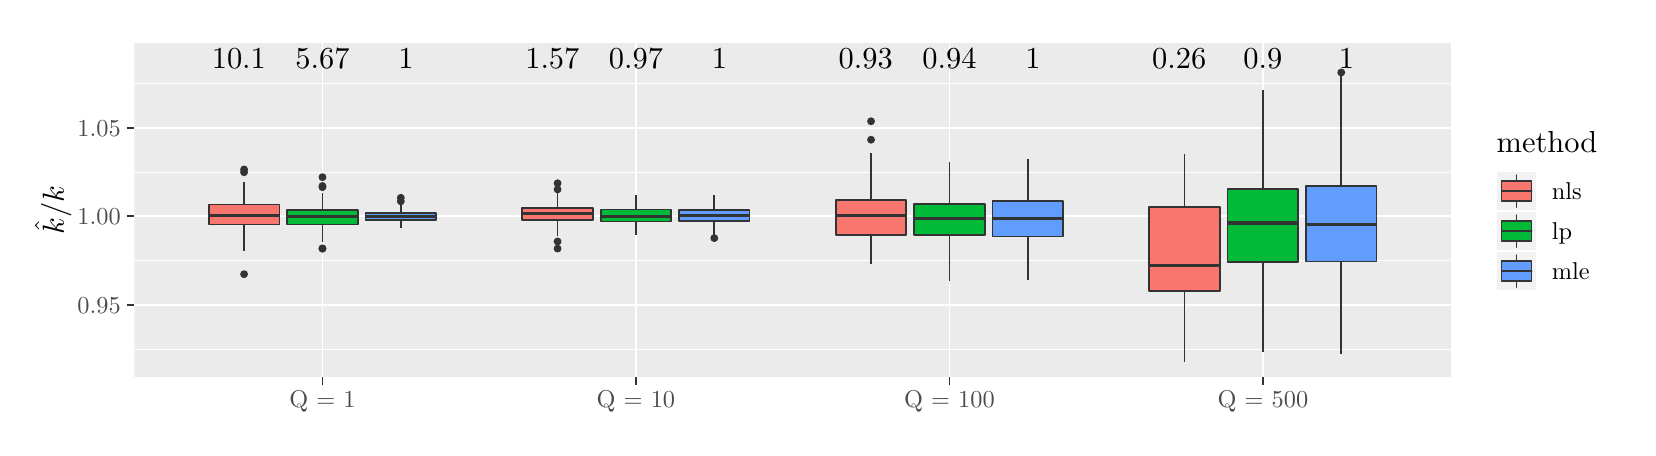
\begin{tikzpicture}[x=1pt,y=1pt]
\definecolor{fillColor}{RGB}{255,255,255}
\path[use as bounding box,fill=fillColor,fill opacity=0.00] (0,0) rectangle (578.16,144.54);
\begin{scope}
\path[clip] (  0.00,  0.00) rectangle (578.16,144.54);
\definecolor{drawColor}{RGB}{255,255,255}
\definecolor{fillColor}{RGB}{255,255,255}

\path[draw=drawColor,line width= 0.6pt,line join=round,line cap=round,fill=fillColor] (  0.00,  0.00) rectangle (578.16,144.54);
\end{scope}
\begin{scope}
\path[clip] ( 38.56, 18.22) rectangle (514.31,139.04);
\definecolor{fillColor}{gray}{0.92}

\path[fill=fillColor] ( 38.56, 18.22) rectangle (514.31,139.04);
\definecolor{drawColor}{RGB}{255,255,255}

\path[draw=drawColor,line width= 0.3pt,line join=round] ( 38.56, 28.41) --
	(514.31, 28.41);

\path[draw=drawColor,line width= 0.3pt,line join=round] ( 38.56, 60.40) --
	(514.31, 60.40);

\path[draw=drawColor,line width= 0.3pt,line join=round] ( 38.56, 92.40) --
	(514.31, 92.40);

\path[draw=drawColor,line width= 0.3pt,line join=round] ( 38.56,124.40) --
	(514.31,124.40);

\path[draw=drawColor,line width= 0.6pt,line join=round] ( 38.56, 44.40) --
	(514.31, 44.40);

\path[draw=drawColor,line width= 0.6pt,line join=round] ( 38.56, 76.40) --
	(514.31, 76.40);

\path[draw=drawColor,line width= 0.6pt,line join=round] ( 38.56,108.40) --
	(514.31,108.40);

\path[draw=drawColor,line width= 0.6pt,line join=round] (106.52, 18.22) --
	(106.52,139.04);

\path[draw=drawColor,line width= 0.6pt,line join=round] (219.79, 18.22) --
	(219.79,139.04);

\path[draw=drawColor,line width= 0.6pt,line join=round] (333.07, 18.22) --
	(333.07,139.04);

\path[draw=drawColor,line width= 0.6pt,line join=round] (446.34, 18.22) --
	(446.34,139.04);
\definecolor{drawColor}{gray}{0.20}
\definecolor{fillColor}{gray}{0.20}

\path[draw=drawColor,line width= 0.4pt,line join=round,line cap=round,fill=fillColor] ( 78.20, 55.46) circle (  1.21);

\path[draw=drawColor,line width= 0.4pt,line join=round,line cap=round,fill=fillColor] ( 78.20, 92.30) circle (  1.21);

\path[draw=drawColor,line width= 0.4pt,line join=round,line cap=round,fill=fillColor] ( 78.20, 93.32) circle (  1.21);

\path[draw=drawColor,line width= 0.6pt,line join=round] ( 78.20, 80.59) -- ( 78.20, 88.87);

\path[draw=drawColor,line width= 0.6pt,line join=round] ( 78.20, 73.42) -- ( 78.20, 63.72);
\definecolor{fillColor}{RGB}{248,118,109}

\path[draw=drawColor,line width= 0.6pt,line join=round,line cap=round,fill=fillColor] ( 65.46, 80.59) --
	( 65.46, 73.42) --
	( 90.94, 73.42) --
	( 90.94, 80.59) --
	( 65.46, 80.59) --
	cycle;

\path[draw=drawColor,line width= 1.1pt,line join=round] ( 65.46, 76.59) -- ( 90.94, 76.59);
\definecolor{fillColor}{gray}{0.20}

\path[draw=drawColor,line width= 0.4pt,line join=round,line cap=round,fill=fillColor] (106.52, 87.34) circle (  1.21);

\path[draw=drawColor,line width= 0.4pt,line join=round,line cap=round,fill=fillColor] (106.52, 86.90) circle (  1.21);

\path[draw=drawColor,line width= 0.4pt,line join=round,line cap=round,fill=fillColor] (106.52, 64.78) circle (  1.21);

\path[draw=drawColor,line width= 0.4pt,line join=round,line cap=round,fill=fillColor] (106.52, 64.68) circle (  1.21);

\path[draw=drawColor,line width= 0.4pt,line join=round,line cap=round,fill=fillColor] (106.52, 90.52) circle (  1.21);

\path[draw=drawColor,line width= 0.6pt,line join=round] (106.52, 78.57) -- (106.52, 84.84);

\path[draw=drawColor,line width= 0.6pt,line join=round] (106.52, 73.40) -- (106.52, 67.20);
\definecolor{fillColor}{RGB}{0,186,56}

\path[draw=drawColor,line width= 0.6pt,line join=round,line cap=round,fill=fillColor] ( 93.78, 78.57) --
	( 93.78, 73.40) --
	(119.26, 73.40) --
	(119.26, 78.57) --
	( 93.78, 78.57) --
	cycle;

\path[draw=drawColor,line width= 1.1pt,line join=round] ( 93.78, 76.15) -- (119.26, 76.15);
\definecolor{fillColor}{gray}{0.20}

\path[draw=drawColor,line width= 0.4pt,line join=round,line cap=round,fill=fillColor] (134.84, 81.80) circle (  1.21);

\path[draw=drawColor,line width= 0.4pt,line join=round,line cap=round,fill=fillColor] (134.84, 83.06) circle (  1.21);

\path[draw=drawColor,line width= 0.6pt,line join=round] (134.84, 77.48) -- (134.84, 80.80);

\path[draw=drawColor,line width= 0.6pt,line join=round] (134.84, 75.07) -- (134.84, 72.01);
\definecolor{fillColor}{RGB}{97,156,255}

\path[draw=drawColor,line width= 0.6pt,line join=round,line cap=round,fill=fillColor] (122.09, 77.48) --
	(122.09, 75.07) --
	(147.58, 75.07) --
	(147.58, 77.48) --
	(122.09, 77.48) --
	cycle;

\path[draw=drawColor,line width= 1.1pt,line join=round] (122.09, 76.33) -- (147.58, 76.33);
\definecolor{fillColor}{gray}{0.20}

\path[draw=drawColor,line width= 0.4pt,line join=round,line cap=round,fill=fillColor] (191.48, 67.28) circle (  1.21);

\path[draw=drawColor,line width= 0.4pt,line join=round,line cap=round,fill=fillColor] (191.48, 86.10) circle (  1.21);

\path[draw=drawColor,line width= 0.4pt,line join=round,line cap=round,fill=fillColor] (191.48, 88.32) circle (  1.21);

\path[draw=drawColor,line width= 0.4pt,line join=round,line cap=round,fill=fillColor] (191.48, 64.72) circle (  1.21);

\path[draw=drawColor,line width= 0.6pt,line join=round] (191.48, 79.34) -- (191.48, 85.03);

\path[draw=drawColor,line width= 0.6pt,line join=round] (191.48, 74.95) -- (191.48, 69.30);
\definecolor{fillColor}{RGB}{248,118,109}

\path[draw=drawColor,line width= 0.6pt,line join=round,line cap=round,fill=fillColor] (178.73, 79.34) --
	(178.73, 74.95) --
	(204.22, 74.95) --
	(204.22, 79.34) --
	(178.73, 79.34) --
	cycle;

\path[draw=drawColor,line width= 1.1pt,line join=round] (178.73, 77.45) -- (204.22, 77.45);

\path[draw=drawColor,line width= 0.6pt,line join=round] (219.79, 78.81) -- (219.79, 84.01);

\path[draw=drawColor,line width= 0.6pt,line join=round] (219.79, 74.53) -- (219.79, 69.58);
\definecolor{fillColor}{RGB}{0,186,56}

\path[draw=drawColor,line width= 0.6pt,line join=round,line cap=round,fill=fillColor] (207.05, 78.81) --
	(207.05, 74.53) --
	(232.54, 74.53) --
	(232.54, 78.81) --
	(207.05, 78.81) --
	cycle;

\path[draw=drawColor,line width= 1.1pt,line join=round] (207.05, 76.43) -- (232.54, 76.43);
\definecolor{fillColor}{gray}{0.20}

\path[draw=drawColor,line width= 0.4pt,line join=round,line cap=round,fill=fillColor] (248.11, 68.50) circle (  1.21);

\path[draw=drawColor,line width= 0.6pt,line join=round] (248.11, 78.57) -- (248.11, 84.08);

\path[draw=drawColor,line width= 0.6pt,line join=round] (248.11, 74.61) -- (248.11, 69.16);
\definecolor{fillColor}{RGB}{97,156,255}

\path[draw=drawColor,line width= 0.6pt,line join=round,line cap=round,fill=fillColor] (235.37, 78.57) --
	(235.37, 74.61) --
	(260.86, 74.61) --
	(260.86, 78.57) --
	(235.37, 78.57) --
	cycle;

\path[draw=drawColor,line width= 1.1pt,line join=round] (235.37, 76.61) -- (260.86, 76.61);
\definecolor{fillColor}{gray}{0.20}

\path[draw=drawColor,line width= 0.4pt,line join=round,line cap=round,fill=fillColor] (304.75,104.05) circle (  1.21);

\path[draw=drawColor,line width= 0.4pt,line join=round,line cap=round,fill=fillColor] (304.75,110.72) circle (  1.21);

\path[draw=drawColor,line width= 0.6pt,line join=round] (304.75, 82.36) -- (304.75, 99.20);

\path[draw=drawColor,line width= 0.6pt,line join=round] (304.75, 69.66) -- (304.75, 59.21);
\definecolor{fillColor}{RGB}{248,118,109}

\path[draw=drawColor,line width= 0.6pt,line join=round,line cap=round,fill=fillColor] (292.01, 82.36) --
	(292.01, 69.66) --
	(317.49, 69.66) --
	(317.49, 82.36) --
	(292.01, 82.36) --
	cycle;

\path[draw=drawColor,line width= 1.1pt,line join=round] (292.01, 76.76) -- (317.49, 76.76);

\path[draw=drawColor,line width= 0.6pt,line join=round] (333.07, 80.87) -- (333.07, 96.15);

\path[draw=drawColor,line width= 0.6pt,line join=round] (333.07, 69.69) -- (333.07, 52.93);
\definecolor{fillColor}{RGB}{0,186,56}

\path[draw=drawColor,line width= 0.6pt,line join=round,line cap=round,fill=fillColor] (320.33, 80.87) --
	(320.33, 69.69) --
	(345.81, 69.69) --
	(345.81, 80.87) --
	(320.33, 80.87) --
	cycle;

\path[draw=drawColor,line width= 1.1pt,line join=round] (320.33, 75.73) -- (345.81, 75.73);

\path[draw=drawColor,line width= 0.6pt,line join=round] (361.39, 81.90) -- (361.39, 96.93);

\path[draw=drawColor,line width= 0.6pt,line join=round] (361.39, 69.14) -- (361.39, 53.31);
\definecolor{fillColor}{RGB}{97,156,255}

\path[draw=drawColor,line width= 0.6pt,line join=round,line cap=round,fill=fillColor] (348.64, 81.90) --
	(348.64, 69.14) --
	(374.13, 69.14) --
	(374.13, 81.90) --
	(348.64, 81.90) --
	cycle;

\path[draw=drawColor,line width= 1.1pt,line join=round] (348.64, 75.50) -- (374.13, 75.50);

\path[draw=drawColor,line width= 0.6pt,line join=round] (418.02, 79.67) -- (418.02, 98.88);

\path[draw=drawColor,line width= 0.6pt,line join=round] (418.02, 49.38) -- (418.02, 23.71);
\definecolor{fillColor}{RGB}{248,118,109}

\path[draw=drawColor,line width= 0.6pt,line join=round,line cap=round,fill=fillColor] (405.28, 79.67) --
	(405.28, 49.38) --
	(430.77, 49.38) --
	(430.77, 79.67) --
	(405.28, 79.67) --
	cycle;

\path[draw=drawColor,line width= 1.1pt,line join=round] (405.28, 58.61) -- (430.77, 58.61);

\path[draw=drawColor,line width= 0.6pt,line join=round] (446.34, 86.16) -- (446.34,122.00);

\path[draw=drawColor,line width= 0.6pt,line join=round] (446.34, 59.95) -- (446.34, 27.19);
\definecolor{fillColor}{RGB}{0,186,56}

\path[draw=drawColor,line width= 0.6pt,line join=round,line cap=round,fill=fillColor] (433.60, 86.16) --
	(433.60, 59.95) --
	(459.09, 59.95) --
	(459.09, 86.16) --
	(433.60, 86.16) --
	cycle;

\path[draw=drawColor,line width= 1.1pt,line join=round] (433.60, 73.95) -- (459.09, 73.95);
\definecolor{fillColor}{gray}{0.20}

\path[draw=drawColor,line width= 0.4pt,line join=round,line cap=round,fill=fillColor] (474.66,128.35) circle (  1.21);

\path[draw=drawColor,line width= 0.6pt,line join=round] (474.66, 87.27) -- (474.66,127.01);

\path[draw=drawColor,line width= 0.6pt,line join=round] (474.66, 60.08) -- (474.66, 26.46);
\definecolor{fillColor}{RGB}{97,156,255}

\path[draw=drawColor,line width= 0.6pt,line join=round,line cap=round,fill=fillColor] (461.92, 87.27) --
	(461.92, 60.08) --
	(487.40, 60.08) --
	(487.40, 87.27) --
	(461.92, 87.27) --
	cycle;

\path[draw=drawColor,line width= 1.1pt,line join=round] (461.92, 73.58) -- (487.40, 73.58);
\definecolor{drawColor}{RGB}{0,0,0}

\node[text=drawColor,anchor=base,inner sep=0pt, outer sep=0pt, scale=  1.10] at (136.73,129.75) {1};

\node[text=drawColor,anchor=base,inner sep=0pt, outer sep=0pt, scale=  1.10] at (106.52,129.75) {5.67};

\node[text=drawColor,anchor=base,inner sep=0pt, outer sep=0pt, scale=  1.10] at ( 76.31,129.75) {10.1};

\node[text=drawColor,anchor=base,inner sep=0pt, outer sep=0pt, scale=  1.10] at (250.00,129.75) {1};

\node[text=drawColor,anchor=base,inner sep=0pt, outer sep=0pt, scale=  1.10] at (219.79,129.75) {0.97};

\node[text=drawColor,anchor=base,inner sep=0pt, outer sep=0pt, scale=  1.10] at (189.59,129.75) {1.57};

\node[text=drawColor,anchor=base,inner sep=0pt, outer sep=0pt, scale=  1.10] at (363.28,129.75) {1};

\node[text=drawColor,anchor=base,inner sep=0pt, outer sep=0pt, scale=  1.10] at (333.07,129.75) {0.94};

\node[text=drawColor,anchor=base,inner sep=0pt, outer sep=0pt, scale=  1.10] at (302.86,129.75) {0.93};

\node[text=drawColor,anchor=base,inner sep=0pt, outer sep=0pt, scale=  1.10] at (476.55,129.75) {1};

\node[text=drawColor,anchor=base,inner sep=0pt, outer sep=0pt, scale=  1.10] at (446.34,129.75) {0.9};

\node[text=drawColor,anchor=base,inner sep=0pt, outer sep=0pt, scale=  1.10] at (416.14,129.75) {0.26};
\end{scope}
\begin{scope}
\path[clip] (  0.00,  0.00) rectangle (578.16,144.54);
\definecolor{drawColor}{gray}{0.30}

\node[text=drawColor,anchor=base east,inner sep=0pt, outer sep=0pt, scale=  0.88] at ( 33.61, 41.37) {0.95};

\node[text=drawColor,anchor=base east,inner sep=0pt, outer sep=0pt, scale=  0.88] at ( 33.61, 73.37) {1.00};

\node[text=drawColor,anchor=base east,inner sep=0pt, outer sep=0pt, scale=  0.88] at ( 33.61,105.37) {1.05};
\end{scope}
\begin{scope}
\path[clip] (  0.00,  0.00) rectangle (578.16,144.54);
\definecolor{drawColor}{gray}{0.20}

\path[draw=drawColor,line width= 0.6pt,line join=round] ( 35.81, 44.40) --
	( 38.56, 44.40);

\path[draw=drawColor,line width= 0.6pt,line join=round] ( 35.81, 76.40) --
	( 38.56, 76.40);

\path[draw=drawColor,line width= 0.6pt,line join=round] ( 35.81,108.40) --
	( 38.56,108.40);
\end{scope}
\begin{scope}
\path[clip] (  0.00,  0.00) rectangle (578.16,144.54);
\definecolor{drawColor}{gray}{0.20}

\path[draw=drawColor,line width= 0.6pt,line join=round] (106.52, 15.47) --
	(106.52, 18.22);

\path[draw=drawColor,line width= 0.6pt,line join=round] (219.79, 15.47) --
	(219.79, 18.22);

\path[draw=drawColor,line width= 0.6pt,line join=round] (333.07, 15.47) --
	(333.07, 18.22);

\path[draw=drawColor,line width= 0.6pt,line join=round] (446.34, 15.47) --
	(446.34, 18.22);
\end{scope}
\begin{scope}
\path[clip] (  0.00,  0.00) rectangle (578.16,144.54);
\definecolor{drawColor}{gray}{0.30}

\node[text=drawColor,anchor=base,inner sep=0pt, outer sep=0pt, scale=  0.88] at (106.52,  7.21) {Q = 1};

\node[text=drawColor,anchor=base,inner sep=0pt, outer sep=0pt, scale=  0.88] at (219.79,  7.21) {Q = 10};

\node[text=drawColor,anchor=base,inner sep=0pt, outer sep=0pt, scale=  0.88] at (333.07,  7.21) {Q = 100};

\node[text=drawColor,anchor=base,inner sep=0pt, outer sep=0pt, scale=  0.88] at (446.34,  7.21) {Q = 500};
\end{scope}
\begin{scope}
\path[clip] (  0.00,  0.00) rectangle (578.16,144.54);
\definecolor{drawColor}{RGB}{0,0,0}

\node[text=drawColor,rotate= 90.00,anchor=base,inner sep=0pt, outer sep=0pt, scale=  1.10] at ( 13.08, 78.63) {$\hat{k}/k$};
\end{scope}
\begin{scope}
\path[clip] (  0.00,  0.00) rectangle (578.16,144.54);
\definecolor{fillColor}{RGB}{255,255,255}

\path[fill=fillColor] (525.31, 43.84) rectangle (572.66,113.42);
\end{scope}
\begin{scope}
\path[clip] (  0.00,  0.00) rectangle (578.16,144.54);
\definecolor{drawColor}{RGB}{0,0,0}

\node[text=drawColor,anchor=base west,inner sep=0pt, outer sep=0pt, scale=  1.10] at (530.81, 99.27) {method};
\end{scope}
\begin{scope}
\path[clip] (  0.00,  0.00) rectangle (578.16,144.54);
\definecolor{drawColor}{RGB}{255,255,255}
\definecolor{fillColor}{gray}{0.95}

\path[draw=drawColor,line width= 0.6pt,line join=round,line cap=round,fill=fillColor] (530.81, 78.25) rectangle (545.26, 92.70);
\end{scope}
\begin{scope}
\path[clip] (  0.00,  0.00) rectangle (578.16,144.54);
\definecolor{drawColor}{gray}{0.20}

\path[draw=drawColor,line width= 0.6pt,line join=round,line cap=round] (538.03, 79.70) --
	(538.03, 81.86);

\path[draw=drawColor,line width= 0.6pt,line join=round,line cap=round] (538.03, 89.09) --
	(538.03, 91.26);
\definecolor{fillColor}{RGB}{248,118,109}

\path[draw=drawColor,line width= 0.6pt,line join=round,line cap=round,fill=fillColor] (532.61, 81.86) rectangle (543.45, 89.09);

\path[draw=drawColor,line width= 0.6pt,line join=round,line cap=round] (532.61, 85.48) --
	(543.45, 85.48);
\end{scope}
\begin{scope}
\path[clip] (  0.00,  0.00) rectangle (578.16,144.54);
\definecolor{drawColor}{RGB}{255,255,255}
\definecolor{fillColor}{gray}{0.95}

\path[draw=drawColor,line width= 0.6pt,line join=round,line cap=round,fill=fillColor] (530.81, 63.80) rectangle (545.26, 78.25);
\end{scope}
\begin{scope}
\path[clip] (  0.00,  0.00) rectangle (578.16,144.54);
\definecolor{drawColor}{gray}{0.20}

\path[draw=drawColor,line width= 0.6pt,line join=round,line cap=round] (538.03, 65.24) --
	(538.03, 67.41);

\path[draw=drawColor,line width= 0.6pt,line join=round,line cap=round] (538.03, 74.64) --
	(538.03, 76.81);
\definecolor{fillColor}{RGB}{0,186,56}

\path[draw=drawColor,line width= 0.6pt,line join=round,line cap=round,fill=fillColor] (532.61, 67.41) rectangle (543.45, 74.64);

\path[draw=drawColor,line width= 0.6pt,line join=round,line cap=round] (532.61, 71.02) --
	(543.45, 71.02);
\end{scope}
\begin{scope}
\path[clip] (  0.00,  0.00) rectangle (578.16,144.54);
\definecolor{drawColor}{RGB}{255,255,255}
\definecolor{fillColor}{gray}{0.95}

\path[draw=drawColor,line width= 0.6pt,line join=round,line cap=round,fill=fillColor] (530.81, 49.34) rectangle (545.26, 63.80);
\end{scope}
\begin{scope}
\path[clip] (  0.00,  0.00) rectangle (578.16,144.54);
\definecolor{drawColor}{gray}{0.20}

\path[draw=drawColor,line width= 0.6pt,line join=round,line cap=round] (538.03, 50.79) --
	(538.03, 52.96);

\path[draw=drawColor,line width= 0.6pt,line join=round,line cap=round] (538.03, 60.18) --
	(538.03, 62.35);
\definecolor{fillColor}{RGB}{97,156,255}

\path[draw=drawColor,line width= 0.6pt,line join=round,line cap=round,fill=fillColor] (532.61, 52.96) rectangle (543.45, 60.18);

\path[draw=drawColor,line width= 0.6pt,line join=round,line cap=round] (532.61, 56.57) --
	(543.45, 56.57);
\end{scope}
\begin{scope}
\path[clip] (  0.00,  0.00) rectangle (578.16,144.54);
\definecolor{drawColor}{RGB}{0,0,0}

\node[text=drawColor,anchor=base west,inner sep=0pt, outer sep=0pt, scale=  0.88] at (550.76, 82.45) {nls};
\end{scope}
\begin{scope}
\path[clip] (  0.00,  0.00) rectangle (578.16,144.54);
\definecolor{drawColor}{RGB}{0,0,0}

\node[text=drawColor,anchor=base west,inner sep=0pt, outer sep=0pt, scale=  0.88] at (550.76, 67.99) {lp};
\end{scope}
\begin{scope}
\path[clip] (  0.00,  0.00) rectangle (578.16,144.54);
\definecolor{drawColor}{RGB}{0,0,0}

\node[text=drawColor,anchor=base west,inner sep=0pt, outer sep=0pt, scale=  0.88] at (550.76, 53.54) {mle};
\end{scope}
\end{tikzpicture}
}
  \end{subfigure}
  \hfill
  \begin{subfigure}
    \centering
    \resizebox{1.1\linewidth}{!}{% Created by tikzDevice version 0.12.3 on 2019-09-28 13:50:10
% !TEX encoding = UTF-8 Unicode
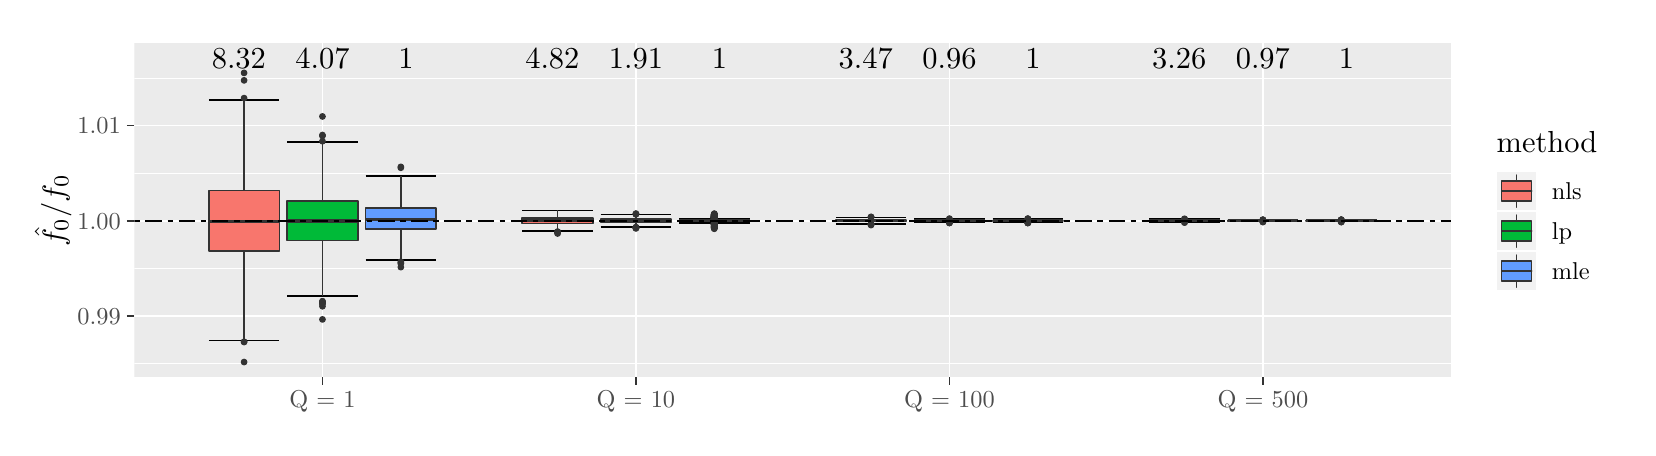
\begin{tikzpicture}[x=1pt,y=1pt]
\definecolor{fillColor}{RGB}{255,255,255}
\path[use as bounding box,fill=fillColor,fill opacity=0.00] (0,0) rectangle (578.16,144.54);
\begin{scope}
\path[clip] (  0.00,  0.00) rectangle (578.16,144.54);
\definecolor{drawColor}{RGB}{255,255,255}
\definecolor{fillColor}{RGB}{255,255,255}

\path[draw=drawColor,line width= 0.6pt,line join=round,line cap=round,fill=fillColor] (  0.00,  0.00) rectangle (578.16,144.54);
\end{scope}
\begin{scope}
\path[clip] ( 38.56, 18.22) rectangle (514.31,139.04);
\definecolor{fillColor}{gray}{0.92}

\path[fill=fillColor] ( 38.56, 18.22) rectangle (514.31,139.04);
\definecolor{drawColor}{RGB}{255,255,255}

\path[draw=drawColor,line width= 0.3pt,line join=round] ( 38.56, 23.12) --
	(514.31, 23.12);

\path[draw=drawColor,line width= 0.3pt,line join=round] ( 38.56, 57.54) --
	(514.31, 57.54);

\path[draw=drawColor,line width= 0.3pt,line join=round] ( 38.56, 91.95) --
	(514.31, 91.95);

\path[draw=drawColor,line width= 0.3pt,line join=round] ( 38.56,126.37) --
	(514.31,126.37);

\path[draw=drawColor,line width= 0.6pt,line join=round] ( 38.56, 40.33) --
	(514.31, 40.33);

\path[draw=drawColor,line width= 0.6pt,line join=round] ( 38.56, 74.75) --
	(514.31, 74.75);

\path[draw=drawColor,line width= 0.6pt,line join=round] ( 38.56,109.16) --
	(514.31,109.16);

\path[draw=drawColor,line width= 0.6pt,line join=round] (106.52, 18.22) --
	(106.52,139.04);

\path[draw=drawColor,line width= 0.6pt,line join=round] (219.79, 18.22) --
	(219.79,139.04);

\path[draw=drawColor,line width= 0.6pt,line join=round] (333.07, 18.22) --
	(333.07,139.04);

\path[draw=drawColor,line width= 0.6pt,line join=round] (446.34, 18.22) --
	(446.34,139.04);
\definecolor{drawColor}{RGB}{0,0,0}

\path[draw=drawColor,line width= 0.6pt,line join=round] ( 65.46,118.40) --
	( 90.94,118.40);

\path[draw=drawColor,line width= 0.6pt,line join=round] ( 78.20,118.40) --
	( 78.20, 31.50);

\path[draw=drawColor,line width= 0.6pt,line join=round] ( 65.46, 31.50) --
	( 90.94, 31.50);

\path[draw=drawColor,line width= 0.6pt,line join=round] ( 93.78,103.18) --
	(119.26,103.18);

\path[draw=drawColor,line width= 0.6pt,line join=round] (106.52,103.18) --
	(106.52, 47.51);

\path[draw=drawColor,line width= 0.6pt,line join=round] ( 93.78, 47.51) --
	(119.26, 47.51);

\path[draw=drawColor,line width= 0.6pt,line join=round] (122.09, 91.00) --
	(147.58, 91.00);

\path[draw=drawColor,line width= 0.6pt,line join=round] (134.84, 91.00) --
	(134.84, 60.48);

\path[draw=drawColor,line width= 0.6pt,line join=round] (122.09, 60.48) --
	(147.58, 60.48);

\path[draw=drawColor,line width= 0.6pt,line join=round] (178.73, 78.49) --
	(204.22, 78.49);

\path[draw=drawColor,line width= 0.6pt,line join=round] (191.48, 78.49) --
	(191.48, 71.04);

\path[draw=drawColor,line width= 0.6pt,line join=round] (178.73, 71.04) --
	(204.22, 71.04);

\path[draw=drawColor,line width= 0.6pt,line join=round] (207.05, 77.00) --
	(232.54, 77.00);

\path[draw=drawColor,line width= 0.6pt,line join=round] (219.79, 77.00) --
	(219.79, 72.45);

\path[draw=drawColor,line width= 0.6pt,line join=round] (207.05, 72.45) --
	(232.54, 72.45);

\path[draw=drawColor,line width= 0.6pt,line join=round] (235.37, 75.44) --
	(260.86, 75.44);

\path[draw=drawColor,line width= 0.6pt,line join=round] (248.11, 75.44) --
	(248.11, 74.01);

\path[draw=drawColor,line width= 0.6pt,line join=round] (235.37, 74.01) --
	(260.86, 74.01);

\path[draw=drawColor,line width= 0.6pt,line join=round] (292.01, 75.94) --
	(317.49, 75.94);

\path[draw=drawColor,line width= 0.6pt,line join=round] (304.75, 75.94) --
	(304.75, 73.55);

\path[draw=drawColor,line width= 0.6pt,line join=round] (292.01, 73.55) --
	(317.49, 73.55);

\path[draw=drawColor,line width= 0.6pt,line join=round] (320.33, 75.40) --
	(345.81, 75.40);

\path[draw=drawColor,line width= 0.6pt,line join=round] (333.07, 75.40) --
	(333.07, 74.10);

\path[draw=drawColor,line width= 0.6pt,line join=round] (320.33, 74.10) --
	(345.81, 74.10);

\path[draw=drawColor,line width= 0.6pt,line join=round] (348.64, 75.40) --
	(374.13, 75.40);

\path[draw=drawColor,line width= 0.6pt,line join=round] (361.39, 75.40) --
	(361.39, 74.11);

\path[draw=drawColor,line width= 0.6pt,line join=round] (348.64, 74.11) --
	(374.13, 74.11);

\path[draw=drawColor,line width= 0.6pt,line join=round] (405.28, 75.30) --
	(430.77, 75.30);

\path[draw=drawColor,line width= 0.6pt,line join=round] (418.02, 75.30) --
	(418.02, 74.22);

\path[draw=drawColor,line width= 0.6pt,line join=round] (405.28, 74.22) --
	(430.77, 74.22);

\path[draw=drawColor,line width= 0.6pt,line join=round] (433.60, 75.04) --
	(459.09, 75.04);

\path[draw=drawColor,line width= 0.6pt,line join=round] (446.34, 75.04) --
	(446.34, 74.45);

\path[draw=drawColor,line width= 0.6pt,line join=round] (433.60, 74.45) --
	(459.09, 74.45);

\path[draw=drawColor,line width= 0.6pt,line join=round] (461.92, 75.04) --
	(487.40, 75.04);

\path[draw=drawColor,line width= 0.6pt,line join=round] (474.66, 75.04) --
	(474.66, 74.46);

\path[draw=drawColor,line width= 0.6pt,line join=round] (461.92, 74.46) --
	(487.40, 74.46);
\definecolor{drawColor}{gray}{0.20}
\definecolor{fillColor}{gray}{0.20}

\path[draw=drawColor,line width= 0.4pt,line join=round,line cap=round,fill=fillColor] ( 78.20,119.08) circle (  1.02);

\path[draw=drawColor,line width= 0.4pt,line join=round,line cap=round,fill=fillColor] ( 78.20, 23.71) circle (  1.02);

\path[draw=drawColor,line width= 0.4pt,line join=round,line cap=round,fill=fillColor] ( 78.20, 30.97) circle (  1.02);

\path[draw=drawColor,line width= 0.4pt,line join=round,line cap=round,fill=fillColor] ( 78.20,125.50) circle (  1.02);

\path[draw=drawColor,line width= 0.4pt,line join=round,line cap=round,fill=fillColor] ( 78.20,128.20) circle (  1.02);

\path[draw=drawColor,line width= 0.4pt,line join=round,line cap=round,fill=fillColor] ( 78.20, 31.02) circle (  1.02);

\path[draw=drawColor,line width= 0.6pt,line join=round] ( 78.20, 85.75) -- ( 78.20,118.40);

\path[draw=drawColor,line width= 0.6pt,line join=round] ( 78.20, 63.90) -- ( 78.20, 31.50);
\definecolor{fillColor}{RGB}{248,118,109}

\path[draw=drawColor,line width= 0.6pt,line join=round,line cap=round,fill=fillColor] ( 65.46, 85.75) --
	( 65.46, 63.90) --
	( 90.94, 63.90) --
	( 90.94, 85.75) --
	( 65.46, 85.75) --
	cycle;

\path[draw=drawColor,line width= 1.1pt,line join=round] ( 65.46, 74.39) -- ( 90.94, 74.39);
\definecolor{fillColor}{gray}{0.20}

\path[draw=drawColor,line width= 0.4pt,line join=round,line cap=round,fill=fillColor] (106.52,105.41) circle (  1.02);

\path[draw=drawColor,line width= 0.4pt,line join=round,line cap=round,fill=fillColor] (106.52, 45.72) circle (  1.02);

\path[draw=drawColor,line width= 0.4pt,line join=round,line cap=round,fill=fillColor] (106.52,105.74) circle (  1.02);

\path[draw=drawColor,line width= 0.4pt,line join=round,line cap=round,fill=fillColor] (106.52,112.46) circle (  1.02);

\path[draw=drawColor,line width= 0.4pt,line join=round,line cap=round,fill=fillColor] (106.52, 45.26) circle (  1.02);

\path[draw=drawColor,line width= 0.4pt,line join=round,line cap=round,fill=fillColor] (106.52,103.51) circle (  1.02);

\path[draw=drawColor,line width= 0.4pt,line join=round,line cap=round,fill=fillColor] (106.52, 45.31) circle (  1.02);

\path[draw=drawColor,line width= 0.4pt,line join=round,line cap=round,fill=fillColor] (106.52, 39.12) circle (  1.02);

\path[draw=drawColor,line width= 0.4pt,line join=round,line cap=round,fill=fillColor] (106.52, 43.88) circle (  1.02);

\path[draw=drawColor,line width= 0.4pt,line join=round,line cap=round,fill=fillColor] (106.52, 45.02) circle (  1.02);

\path[draw=drawColor,line width= 0.4pt,line join=round,line cap=round,fill=fillColor] (106.52, 44.74) circle (  1.02);

\path[draw=drawColor,line width= 0.4pt,line join=round,line cap=round,fill=fillColor] (106.52, 45.22) circle (  1.02);

\path[draw=drawColor,line width= 0.6pt,line join=round] (106.52, 81.85) -- (106.52,103.18);

\path[draw=drawColor,line width= 0.6pt,line join=round] (106.52, 67.59) -- (106.52, 47.51);
\definecolor{fillColor}{RGB}{0,186,56}

\path[draw=drawColor,line width= 0.6pt,line join=round,line cap=round,fill=fillColor] ( 93.78, 81.85) --
	( 93.78, 67.59) --
	(119.26, 67.59) --
	(119.26, 81.85) --
	( 93.78, 81.85) --
	cycle;

\path[draw=drawColor,line width= 1.1pt,line join=round] ( 93.78, 74.68) -- (119.26, 74.68);
\definecolor{fillColor}{gray}{0.20}

\path[draw=drawColor,line width= 0.4pt,line join=round,line cap=round,fill=fillColor] (134.84, 93.92) circle (  1.02);

\path[draw=drawColor,line width= 0.4pt,line join=round,line cap=round,fill=fillColor] (134.84, 58.01) circle (  1.02);

\path[draw=drawColor,line width= 0.4pt,line join=round,line cap=round,fill=fillColor] (134.84, 59.34) circle (  1.02);

\path[draw=drawColor,line width= 0.4pt,line join=round,line cap=round,fill=fillColor] (134.84, 94.25) circle (  1.02);

\path[draw=drawColor,line width= 0.4pt,line join=round,line cap=round,fill=fillColor] (134.84, 59.54) circle (  1.02);

\path[draw=drawColor,line width= 0.4pt,line join=round,line cap=round,fill=fillColor] (134.84, 59.95) circle (  1.02);

\path[draw=drawColor,line width= 0.6pt,line join=round] (134.84, 79.45) -- (134.84, 91.00);

\path[draw=drawColor,line width= 0.6pt,line join=round] (134.84, 71.71) -- (134.84, 60.48);
\definecolor{fillColor}{RGB}{97,156,255}

\path[draw=drawColor,line width= 0.6pt,line join=round,line cap=round,fill=fillColor] (122.09, 79.45) --
	(122.09, 71.71) --
	(147.58, 71.71) --
	(147.58, 79.45) --
	(122.09, 79.45) --
	cycle;

\path[draw=drawColor,line width= 1.1pt,line join=round] (122.09, 75.39) -- (147.58, 75.39);
\definecolor{fillColor}{gray}{0.20}

\path[draw=drawColor,line width= 0.4pt,line join=round,line cap=round,fill=fillColor] (191.48, 70.81) circle (  1.02);

\path[draw=drawColor,line width= 0.4pt,line join=round,line cap=round,fill=fillColor] (191.48, 70.17) circle (  1.02);

\path[draw=drawColor,line width= 0.4pt,line join=round,line cap=round,fill=fillColor] (191.48, 70.48) circle (  1.02);

\path[draw=drawColor,line width= 0.4pt,line join=round,line cap=round,fill=fillColor] (191.48, 70.79) circle (  1.02);

\path[draw=drawColor,line width= 0.6pt,line join=round] (191.48, 75.68) -- (191.48, 78.49);

\path[draw=drawColor,line width= 0.6pt,line join=round] (191.48, 73.75) -- (191.48, 71.04);
\definecolor{fillColor}{RGB}{248,118,109}

\path[draw=drawColor,line width= 0.6pt,line join=round,line cap=round,fill=fillColor] (178.73, 75.68) --
	(178.73, 73.75) --
	(204.22, 73.75) --
	(204.22, 75.68) --
	(178.73, 75.68) --
	cycle;

\path[draw=drawColor,line width= 1.1pt,line join=round] (178.73, 74.72) -- (204.22, 74.72);
\definecolor{fillColor}{gray}{0.20}

\path[draw=drawColor,line width= 0.4pt,line join=round,line cap=round,fill=fillColor] (219.79, 77.36) circle (  1.02);

\path[draw=drawColor,line width= 0.4pt,line join=round,line cap=round,fill=fillColor] (219.79, 72.10) circle (  1.02);

\path[draw=drawColor,line width= 0.4pt,line join=round,line cap=round,fill=fillColor] (219.79, 72.33) circle (  1.02);

\path[draw=drawColor,line width= 0.4pt,line join=round,line cap=round,fill=fillColor] (219.79, 77.16) circle (  1.02);

\path[draw=drawColor,line width= 0.4pt,line join=round,line cap=round,fill=fillColor] (219.79, 72.30) circle (  1.02);

\path[draw=drawColor,line width= 0.4pt,line join=round,line cap=round,fill=fillColor] (219.79, 72.03) circle (  1.02);

\path[draw=drawColor,line width= 0.4pt,line join=round,line cap=round,fill=fillColor] (219.79, 77.12) circle (  1.02);

\path[draw=drawColor,line width= 0.4pt,line join=round,line cap=round,fill=fillColor] (219.79, 72.40) circle (  1.02);

\path[draw=drawColor,line width= 0.4pt,line join=round,line cap=round,fill=fillColor] (219.79, 72.31) circle (  1.02);

\path[draw=drawColor,line width= 0.4pt,line join=round,line cap=round,fill=fillColor] (219.79, 72.37) circle (  1.02);

\path[draw=drawColor,line width= 0.6pt,line join=round] (219.79, 75.33) -- (219.79, 77.00);

\path[draw=drawColor,line width= 0.6pt,line join=round] (219.79, 74.17) -- (219.79, 72.45);
\definecolor{fillColor}{RGB}{0,186,56}

\path[draw=drawColor,line width= 0.6pt,line join=round,line cap=round,fill=fillColor] (207.05, 75.33) --
	(207.05, 74.17) --
	(232.54, 74.17) --
	(232.54, 75.33) --
	(207.05, 75.33) --
	cycle;

\path[draw=drawColor,line width= 1.1pt,line join=round] (207.05, 74.75) -- (232.54, 74.75);
\definecolor{fillColor}{gray}{0.20}

\path[draw=drawColor,line width= 0.4pt,line join=round,line cap=round,fill=fillColor] (248.11, 76.17) circle (  1.02);

\path[draw=drawColor,line width= 0.4pt,line join=round,line cap=round,fill=fillColor] (248.11, 72.43) circle (  1.02);

\path[draw=drawColor,line width= 0.4pt,line join=round,line cap=round,fill=fillColor] (248.11, 76.15) circle (  1.02);

\path[draw=drawColor,line width= 0.4pt,line join=round,line cap=round,fill=fillColor] (248.11, 75.44) circle (  1.02);

\path[draw=drawColor,line width= 0.4pt,line join=round,line cap=round,fill=fillColor] (248.11, 73.54) circle (  1.02);

\path[draw=drawColor,line width= 0.4pt,line join=round,line cap=round,fill=fillColor] (248.11, 73.97) circle (  1.02);

\path[draw=drawColor,line width= 0.4pt,line join=round,line cap=round,fill=fillColor] (248.11, 73.81) circle (  1.02);

\path[draw=drawColor,line width= 0.4pt,line join=round,line cap=round,fill=fillColor] (248.11, 76.44) circle (  1.02);

\path[draw=drawColor,line width= 0.4pt,line join=round,line cap=round,fill=fillColor] (248.11, 73.67) circle (  1.02);

\path[draw=drawColor,line width= 0.4pt,line join=round,line cap=round,fill=fillColor] (248.11, 76.06) circle (  1.02);

\path[draw=drawColor,line width= 0.4pt,line join=round,line cap=round,fill=fillColor] (248.11, 75.87) circle (  1.02);

\path[draw=drawColor,line width= 0.4pt,line join=round,line cap=round,fill=fillColor] (248.11, 75.58) circle (  1.02);

\path[draw=drawColor,line width= 0.4pt,line join=round,line cap=round,fill=fillColor] (248.11, 76.05) circle (  1.02);

\path[draw=drawColor,line width= 0.4pt,line join=round,line cap=round,fill=fillColor] (248.11, 76.64) circle (  1.02);

\path[draw=drawColor,line width= 0.4pt,line join=round,line cap=round,fill=fillColor] (248.11, 75.46) circle (  1.02);

\path[draw=drawColor,line width= 0.4pt,line join=round,line cap=round,fill=fillColor] (248.11, 75.82) circle (  1.02);

\path[draw=drawColor,line width= 0.4pt,line join=round,line cap=round,fill=fillColor] (248.11, 75.83) circle (  1.02);

\path[draw=drawColor,line width= 0.4pt,line join=round,line cap=round,fill=fillColor] (248.11, 75.65) circle (  1.02);

\path[draw=drawColor,line width= 0.4pt,line join=round,line cap=round,fill=fillColor] (248.11, 75.81) circle (  1.02);

\path[draw=drawColor,line width= 0.4pt,line join=round,line cap=round,fill=fillColor] (248.11, 73.16) circle (  1.02);

\path[draw=drawColor,line width= 0.4pt,line join=round,line cap=round,fill=fillColor] (248.11, 77.22) circle (  1.02);

\path[draw=drawColor,line width= 0.4pt,line join=round,line cap=round,fill=fillColor] (248.11, 75.80) circle (  1.02);

\path[draw=drawColor,line width= 0.4pt,line join=round,line cap=round,fill=fillColor] (248.11, 73.97) circle (  1.02);

\path[draw=drawColor,line width= 0.4pt,line join=round,line cap=round,fill=fillColor] (248.11, 75.58) circle (  1.02);

\path[draw=drawColor,line width= 0.4pt,line join=round,line cap=round,fill=fillColor] (248.11, 75.85) circle (  1.02);

\path[draw=drawColor,line width= 0.4pt,line join=round,line cap=round,fill=fillColor] (248.11, 72.36) circle (  1.02);

\path[draw=drawColor,line width= 0.4pt,line join=round,line cap=round,fill=fillColor] (248.11, 76.42) circle (  1.02);

\path[draw=drawColor,line width= 0.4pt,line join=round,line cap=round,fill=fillColor] (248.11, 75.89) circle (  1.02);

\path[draw=drawColor,line width= 0.4pt,line join=round,line cap=round,fill=fillColor] (248.11, 76.03) circle (  1.02);

\path[draw=drawColor,line width= 0.4pt,line join=round,line cap=round,fill=fillColor] (248.11, 76.59) circle (  1.02);

\path[draw=drawColor,line width= 0.4pt,line join=round,line cap=round,fill=fillColor] (248.11, 75.99) circle (  1.02);

\path[draw=drawColor,line width= 0.4pt,line join=round,line cap=round,fill=fillColor] (248.11, 76.16) circle (  1.02);

\path[draw=drawColor,line width= 0.4pt,line join=round,line cap=round,fill=fillColor] (248.11, 76.20) circle (  1.02);

\path[draw=drawColor,line width= 0.4pt,line join=round,line cap=round,fill=fillColor] (248.11, 76.19) circle (  1.02);

\path[draw=drawColor,line width= 0.4pt,line join=round,line cap=round,fill=fillColor] (248.11, 75.46) circle (  1.02);

\path[draw=drawColor,line width= 0.4pt,line join=round,line cap=round,fill=fillColor] (248.11, 75.91) circle (  1.02);

\path[draw=drawColor,line width= 0.4pt,line join=round,line cap=round,fill=fillColor] (248.11, 75.73) circle (  1.02);

\path[draw=drawColor,line width= 0.4pt,line join=round,line cap=round,fill=fillColor] (248.11, 75.92) circle (  1.02);

\path[draw=drawColor,line width= 0.4pt,line join=round,line cap=round,fill=fillColor] (248.11, 75.45) circle (  1.02);

\path[draw=drawColor,line width= 0.4pt,line join=round,line cap=round,fill=fillColor] (248.11, 76.15) circle (  1.02);

\path[draw=drawColor,line width= 0.4pt,line join=round,line cap=round,fill=fillColor] (248.11, 72.57) circle (  1.02);

\path[draw=drawColor,line width= 0.4pt,line join=round,line cap=round,fill=fillColor] (248.11, 71.99) circle (  1.02);

\path[draw=drawColor,line width= 0.4pt,line join=round,line cap=round,fill=fillColor] (248.11, 73.78) circle (  1.02);

\path[draw=drawColor,line width= 0.4pt,line join=round,line cap=round,fill=fillColor] (248.11, 76.22) circle (  1.02);

\path[draw=drawColor,line width= 0.4pt,line join=round,line cap=round,fill=fillColor] (248.11, 75.75) circle (  1.02);

\path[draw=drawColor,line width= 0.4pt,line join=round,line cap=round,fill=fillColor] (248.11, 76.20) circle (  1.02);

\path[draw=drawColor,line width= 0.4pt,line join=round,line cap=round,fill=fillColor] (248.11, 76.21) circle (  1.02);

\path[draw=drawColor,line width= 0.4pt,line join=round,line cap=round,fill=fillColor] (248.11, 75.72) circle (  1.02);

\path[draw=drawColor,line width= 0.4pt,line join=round,line cap=round,fill=fillColor] (248.11, 76.14) circle (  1.02);

\path[draw=drawColor,line width= 0.4pt,line join=round,line cap=round,fill=fillColor] (248.11, 75.74) circle (  1.02);

\path[draw=drawColor,line width= 0.4pt,line join=round,line cap=round,fill=fillColor] (248.11, 75.58) circle (  1.02);

\path[draw=drawColor,line width= 0.4pt,line join=round,line cap=round,fill=fillColor] (248.11, 76.13) circle (  1.02);

\path[draw=drawColor,line width= 0.4pt,line join=round,line cap=round,fill=fillColor] (248.11, 76.97) circle (  1.02);

\path[draw=drawColor,line width= 0.4pt,line join=round,line cap=round,fill=fillColor] (248.11, 73.63) circle (  1.02);

\path[draw=drawColor,line width= 0.4pt,line join=round,line cap=round,fill=fillColor] (248.11, 76.95) circle (  1.02);

\path[draw=drawColor,line width= 0.4pt,line join=round,line cap=round,fill=fillColor] (248.11, 75.71) circle (  1.02);

\path[draw=drawColor,line width= 0.4pt,line join=round,line cap=round,fill=fillColor] (248.11, 76.95) circle (  1.02);

\path[draw=drawColor,line width= 0.4pt,line join=round,line cap=round,fill=fillColor] (248.11, 75.47) circle (  1.02);

\path[draw=drawColor,line width= 0.4pt,line join=round,line cap=round,fill=fillColor] (248.11, 75.82) circle (  1.02);

\path[draw=drawColor,line width= 0.4pt,line join=round,line cap=round,fill=fillColor] (248.11, 75.50) circle (  1.02);

\path[draw=drawColor,line width= 0.4pt,line join=round,line cap=round,fill=fillColor] (248.11, 76.33) circle (  1.02);

\path[draw=drawColor,line width= 0.4pt,line join=round,line cap=round,fill=fillColor] (248.11, 73.94) circle (  1.02);

\path[draw=drawColor,line width= 0.4pt,line join=round,line cap=round,fill=fillColor] (248.11, 75.76) circle (  1.02);

\path[draw=drawColor,line width= 0.4pt,line join=round,line cap=round,fill=fillColor] (248.11, 73.54) circle (  1.02);

\path[draw=drawColor,line width= 0.4pt,line join=round,line cap=round,fill=fillColor] (248.11, 73.61) circle (  1.02);

\path[draw=drawColor,line width= 0.4pt,line join=round,line cap=round,fill=fillColor] (248.11, 73.10) circle (  1.02);

\path[draw=drawColor,line width= 0.4pt,line join=round,line cap=round,fill=fillColor] (248.11, 76.98) circle (  1.02);

\path[draw=drawColor,line width= 0.4pt,line join=round,line cap=round,fill=fillColor] (248.11, 75.94) circle (  1.02);

\path[draw=drawColor,line width= 0.4pt,line join=round,line cap=round,fill=fillColor] (248.11, 76.10) circle (  1.02);

\path[draw=drawColor,line width= 0.4pt,line join=round,line cap=round,fill=fillColor] (248.11, 73.88) circle (  1.02);

\path[draw=drawColor,line width= 0.4pt,line join=round,line cap=round,fill=fillColor] (248.11, 76.44) circle (  1.02);

\path[draw=drawColor,line width= 0.4pt,line join=round,line cap=round,fill=fillColor] (248.11, 75.59) circle (  1.02);

\path[draw=drawColor,line width= 0.4pt,line join=round,line cap=round,fill=fillColor] (248.11, 76.35) circle (  1.02);

\path[draw=drawColor,line width= 0.4pt,line join=round,line cap=round,fill=fillColor] (248.11, 73.91) circle (  1.02);

\path[draw=drawColor,line width= 0.4pt,line join=round,line cap=round,fill=fillColor] (248.11, 72.87) circle (  1.02);

\path[draw=drawColor,line width= 0.4pt,line join=round,line cap=round,fill=fillColor] (248.11, 76.77) circle (  1.02);

\path[draw=drawColor,line width= 0.4pt,line join=round,line cap=round,fill=fillColor] (248.11, 77.02) circle (  1.02);

\path[draw=drawColor,line width= 0.4pt,line join=round,line cap=round,fill=fillColor] (248.11, 75.48) circle (  1.02);

\path[draw=drawColor,line width= 0.4pt,line join=round,line cap=round,fill=fillColor] (248.11, 76.66) circle (  1.02);

\path[draw=drawColor,line width= 0.4pt,line join=round,line cap=round,fill=fillColor] (248.11, 75.69) circle (  1.02);

\path[draw=drawColor,line width= 0.4pt,line join=round,line cap=round,fill=fillColor] (248.11, 76.75) circle (  1.02);

\path[draw=drawColor,line width= 0.4pt,line join=round,line cap=round,fill=fillColor] (248.11, 72.43) circle (  1.02);

\path[draw=drawColor,line width= 0.4pt,line join=round,line cap=round,fill=fillColor] (248.11, 75.73) circle (  1.02);

\path[draw=drawColor,line width= 0.4pt,line join=round,line cap=round,fill=fillColor] (248.11, 75.63) circle (  1.02);

\path[draw=drawColor,line width= 0.4pt,line join=round,line cap=round,fill=fillColor] (248.11, 75.45) circle (  1.02);

\path[draw=drawColor,line width= 0.4pt,line join=round,line cap=round,fill=fillColor] (248.11, 73.53) circle (  1.02);

\path[draw=drawColor,line width= 0.4pt,line join=round,line cap=round,fill=fillColor] (248.11, 75.90) circle (  1.02);

\path[draw=drawColor,line width= 0.4pt,line join=round,line cap=round,fill=fillColor] (248.11, 76.14) circle (  1.02);

\path[draw=drawColor,line width= 0.4pt,line join=round,line cap=round,fill=fillColor] (248.11, 77.33) circle (  1.02);

\path[draw=drawColor,line width= 0.4pt,line join=round,line cap=round,fill=fillColor] (248.11, 77.11) circle (  1.02);

\path[draw=drawColor,line width= 0.4pt,line join=round,line cap=round,fill=fillColor] (248.11, 75.74) circle (  1.02);

\path[draw=drawColor,line width= 0.4pt,line join=round,line cap=round,fill=fillColor] (248.11, 75.92) circle (  1.02);

\path[draw=drawColor,line width= 0.4pt,line join=round,line cap=round,fill=fillColor] (248.11, 76.46) circle (  1.02);

\path[draw=drawColor,line width= 0.4pt,line join=round,line cap=round,fill=fillColor] (248.11, 76.18) circle (  1.02);

\path[draw=drawColor,line width= 0.4pt,line join=round,line cap=round,fill=fillColor] (248.11, 73.44) circle (  1.02);

\path[draw=drawColor,line width= 0.4pt,line join=round,line cap=round,fill=fillColor] (248.11, 75.83) circle (  1.02);

\path[draw=drawColor,line width= 0.4pt,line join=round,line cap=round,fill=fillColor] (248.11, 73.63) circle (  1.02);

\path[draw=drawColor,line width= 0.4pt,line join=round,line cap=round,fill=fillColor] (248.11, 76.12) circle (  1.02);

\path[draw=drawColor,line width= 0.4pt,line join=round,line cap=round,fill=fillColor] (248.11, 75.85) circle (  1.02);

\path[draw=drawColor,line width= 0.4pt,line join=round,line cap=round,fill=fillColor] (248.11, 75.63) circle (  1.02);

\path[draw=drawColor,line width= 0.4pt,line join=round,line cap=round,fill=fillColor] (248.11, 76.43) circle (  1.02);

\path[draw=drawColor,line width= 0.4pt,line join=round,line cap=round,fill=fillColor] (248.11, 71.90) circle (  1.02);

\path[draw=drawColor,line width= 0.4pt,line join=round,line cap=round,fill=fillColor] (248.11, 73.30) circle (  1.02);

\path[draw=drawColor,line width= 0.4pt,line join=round,line cap=round,fill=fillColor] (248.11, 75.71) circle (  1.02);

\path[draw=drawColor,line width= 0.4pt,line join=round,line cap=round,fill=fillColor] (248.11, 76.20) circle (  1.02);

\path[draw=drawColor,line width= 0.4pt,line join=round,line cap=round,fill=fillColor] (248.11, 73.26) circle (  1.02);

\path[draw=drawColor,line width= 0.4pt,line join=round,line cap=round,fill=fillColor] (248.11, 73.39) circle (  1.02);

\path[draw=drawColor,line width= 0.4pt,line join=round,line cap=round,fill=fillColor] (248.11, 75.94) circle (  1.02);

\path[draw=drawColor,line width= 0.4pt,line join=round,line cap=round,fill=fillColor] (248.11, 76.23) circle (  1.02);

\path[draw=drawColor,line width= 0.4pt,line join=round,line cap=round,fill=fillColor] (248.11, 75.45) circle (  1.02);

\path[draw=drawColor,line width= 0.4pt,line join=round,line cap=round,fill=fillColor] (248.11, 76.22) circle (  1.02);

\path[draw=drawColor,line width= 0.4pt,line join=round,line cap=round,fill=fillColor] (248.11, 72.80) circle (  1.02);

\path[draw=drawColor,line width= 0.4pt,line join=round,line cap=round,fill=fillColor] (248.11, 73.84) circle (  1.02);

\path[draw=drawColor,line width= 0.4pt,line join=round,line cap=round,fill=fillColor] (248.11, 72.45) circle (  1.02);

\path[draw=drawColor,line width= 0.4pt,line join=round,line cap=round,fill=fillColor] (248.11, 75.62) circle (  1.02);

\path[draw=drawColor,line width= 0.4pt,line join=round,line cap=round,fill=fillColor] (248.11, 76.07) circle (  1.02);

\path[draw=drawColor,line width= 0.4pt,line join=round,line cap=round,fill=fillColor] (248.11, 76.62) circle (  1.02);

\path[draw=drawColor,line width= 0.4pt,line join=round,line cap=round,fill=fillColor] (248.11, 76.22) circle (  1.02);

\path[draw=drawColor,line width= 0.4pt,line join=round,line cap=round,fill=fillColor] (248.11, 72.95) circle (  1.02);

\path[draw=drawColor,line width= 0.4pt,line join=round,line cap=round,fill=fillColor] (248.11, 75.63) circle (  1.02);

\path[draw=drawColor,line width= 0.4pt,line join=round,line cap=round,fill=fillColor] (248.11, 73.96) circle (  1.02);

\path[draw=drawColor,line width= 0.4pt,line join=round,line cap=round,fill=fillColor] (248.11, 75.65) circle (  1.02);

\path[draw=drawColor,line width= 0.4pt,line join=round,line cap=round,fill=fillColor] (248.11, 75.99) circle (  1.02);

\path[draw=drawColor,line width= 0.4pt,line join=round,line cap=round,fill=fillColor] (248.11, 76.96) circle (  1.02);

\path[draw=drawColor,line width= 0.4pt,line join=round,line cap=round,fill=fillColor] (248.11, 75.48) circle (  1.02);

\path[draw=drawColor,line width= 0.4pt,line join=round,line cap=round,fill=fillColor] (248.11, 76.19) circle (  1.02);

\path[draw=drawColor,line width= 0.4pt,line join=round,line cap=round,fill=fillColor] (248.11, 75.91) circle (  1.02);

\path[draw=drawColor,line width= 0.4pt,line join=round,line cap=round,fill=fillColor] (248.11, 73.30) circle (  1.02);

\path[draw=drawColor,line width= 0.4pt,line join=round,line cap=round,fill=fillColor] (248.11, 72.71) circle (  1.02);

\path[draw=drawColor,line width= 0.4pt,line join=round,line cap=round,fill=fillColor] (248.11, 73.34) circle (  1.02);

\path[draw=drawColor,line width= 0.4pt,line join=round,line cap=round,fill=fillColor] (248.11, 76.46) circle (  1.02);

\path[draw=drawColor,line width= 0.4pt,line join=round,line cap=round,fill=fillColor] (248.11, 73.93) circle (  1.02);

\path[draw=drawColor,line width= 0.4pt,line join=round,line cap=round,fill=fillColor] (248.11, 72.50) circle (  1.02);

\path[draw=drawColor,line width= 0.4pt,line join=round,line cap=round,fill=fillColor] (248.11, 76.03) circle (  1.02);

\path[draw=drawColor,line width= 0.4pt,line join=round,line cap=round,fill=fillColor] (248.11, 75.89) circle (  1.02);

\path[draw=drawColor,line width= 0.4pt,line join=round,line cap=round,fill=fillColor] (248.11, 76.03) circle (  1.02);

\path[draw=drawColor,line width= 0.4pt,line join=round,line cap=round,fill=fillColor] (248.11, 76.41) circle (  1.02);

\path[draw=drawColor,line width= 0.4pt,line join=round,line cap=round,fill=fillColor] (248.11, 76.06) circle (  1.02);

\path[draw=drawColor,line width= 0.4pt,line join=round,line cap=round,fill=fillColor] (248.11, 72.25) circle (  1.02);

\path[draw=drawColor,line width= 0.4pt,line join=round,line cap=round,fill=fillColor] (248.11, 75.78) circle (  1.02);

\path[draw=drawColor,line width= 0.4pt,line join=round,line cap=round,fill=fillColor] (248.11, 76.66) circle (  1.02);

\path[draw=drawColor,line width= 0.4pt,line join=round,line cap=round,fill=fillColor] (248.11, 73.68) circle (  1.02);

\path[draw=drawColor,line width= 0.4pt,line join=round,line cap=round,fill=fillColor] (248.11, 75.46) circle (  1.02);

\path[draw=drawColor,line width= 0.4pt,line join=round,line cap=round,fill=fillColor] (248.11, 73.97) circle (  1.02);

\path[draw=drawColor,line width= 0.4pt,line join=round,line cap=round,fill=fillColor] (248.11, 76.13) circle (  1.02);

\path[draw=drawColor,line width= 0.4pt,line join=round,line cap=round,fill=fillColor] (248.11, 75.74) circle (  1.02);

\path[draw=drawColor,line width= 0.4pt,line join=round,line cap=round,fill=fillColor] (248.11, 73.50) circle (  1.02);

\path[draw=drawColor,line width= 0.4pt,line join=round,line cap=round,fill=fillColor] (248.11, 72.68) circle (  1.02);

\path[draw=drawColor,line width= 0.4pt,line join=round,line cap=round,fill=fillColor] (248.11, 73.47) circle (  1.02);

\path[draw=drawColor,line width= 0.4pt,line join=round,line cap=round,fill=fillColor] (248.11, 76.66) circle (  1.02);

\path[draw=drawColor,line width= 0.4pt,line join=round,line cap=round,fill=fillColor] (248.11, 75.87) circle (  1.02);

\path[draw=drawColor,line width= 0.4pt,line join=round,line cap=round,fill=fillColor] (248.11, 73.49) circle (  1.02);

\path[draw=drawColor,line width= 0.4pt,line join=round,line cap=round,fill=fillColor] (248.11, 75.67) circle (  1.02);

\path[draw=drawColor,line width= 0.4pt,line join=round,line cap=round,fill=fillColor] (248.11, 76.72) circle (  1.02);

\path[draw=drawColor,line width= 0.4pt,line join=round,line cap=round,fill=fillColor] (248.11, 76.02) circle (  1.02);

\path[draw=drawColor,line width= 0.4pt,line join=round,line cap=round,fill=fillColor] (248.11, 76.01) circle (  1.02);

\path[draw=drawColor,line width= 0.4pt,line join=round,line cap=round,fill=fillColor] (248.11, 76.76) circle (  1.02);

\path[draw=drawColor,line width= 0.4pt,line join=round,line cap=round,fill=fillColor] (248.11, 76.45) circle (  1.02);

\path[draw=drawColor,line width= 0.4pt,line join=round,line cap=round,fill=fillColor] (248.11, 75.63) circle (  1.02);

\path[draw=drawColor,line width= 0.4pt,line join=round,line cap=round,fill=fillColor] (248.11, 75.89) circle (  1.02);

\path[draw=drawColor,line width= 0.4pt,line join=round,line cap=round,fill=fillColor] (248.11, 75.88) circle (  1.02);

\path[draw=drawColor,line width= 0.4pt,line join=round,line cap=round,fill=fillColor] (248.11, 75.81) circle (  1.02);

\path[draw=drawColor,line width= 0.6pt,line join=round] (248.11, 74.89) -- (248.11, 75.44);

\path[draw=drawColor,line width= 0.6pt,line join=round] (248.11, 74.53) -- (248.11, 74.01);
\definecolor{fillColor}{RGB}{97,156,255}

\path[draw=drawColor,line width= 0.6pt,line join=round,line cap=round,fill=fillColor] (235.37, 74.89) --
	(235.37, 74.53) --
	(260.86, 74.53) --
	(260.86, 74.89) --
	(235.37, 74.89) --
	cycle;

\path[draw=drawColor,line width= 1.1pt,line join=round] (235.37, 74.70) -- (260.86, 74.70);
\definecolor{fillColor}{gray}{0.20}

\path[draw=drawColor,line width= 0.4pt,line join=round,line cap=round,fill=fillColor] (304.75, 76.17) circle (  1.02);

\path[draw=drawColor,line width= 0.4pt,line join=round,line cap=round,fill=fillColor] (304.75, 73.20) circle (  1.02);

\path[draw=drawColor,line width= 0.4pt,line join=round,line cap=round,fill=fillColor] (304.75, 76.05) circle (  1.02);

\path[draw=drawColor,line width= 0.4pt,line join=round,line cap=round,fill=fillColor] (304.75, 73.52) circle (  1.02);

\path[draw=drawColor,line width= 0.4pt,line join=round,line cap=round,fill=fillColor] (304.75, 73.51) circle (  1.02);

\path[draw=drawColor,line width= 0.4pt,line join=round,line cap=round,fill=fillColor] (304.75, 73.47) circle (  1.02);

\path[draw=drawColor,line width= 0.4pt,line join=round,line cap=round,fill=fillColor] (304.75, 76.05) circle (  1.02);

\path[draw=drawColor,line width= 0.4pt,line join=round,line cap=round,fill=fillColor] (304.75, 73.53) circle (  1.02);

\path[draw=drawColor,line width= 0.6pt,line join=round] (304.75, 75.06) -- (304.75, 75.94);

\path[draw=drawColor,line width= 0.6pt,line join=round] (304.75, 74.45) -- (304.75, 73.55);
\definecolor{fillColor}{RGB}{248,118,109}

\path[draw=drawColor,line width= 0.6pt,line join=round,line cap=round,fill=fillColor] (292.01, 75.06) --
	(292.01, 74.45) --
	(317.49, 74.45) --
	(317.49, 75.06) --
	(292.01, 75.06) --
	cycle;

\path[draw=drawColor,line width= 1.1pt,line join=round] (292.01, 74.75) -- (317.49, 74.75);
\definecolor{fillColor}{gray}{0.20}

\path[draw=drawColor,line width= 0.4pt,line join=round,line cap=round,fill=fillColor] (333.07, 74.06) circle (  1.02);

\path[draw=drawColor,line width= 0.4pt,line join=round,line cap=round,fill=fillColor] (333.07, 75.53) circle (  1.02);

\path[draw=drawColor,line width= 0.4pt,line join=round,line cap=round,fill=fillColor] (333.07, 75.41) circle (  1.02);

\path[draw=drawColor,line width= 0.4pt,line join=round,line cap=round,fill=fillColor] (333.07, 74.03) circle (  1.02);

\path[draw=drawColor,line width= 0.4pt,line join=round,line cap=round,fill=fillColor] (333.07, 73.96) circle (  1.02);

\path[draw=drawColor,line width= 0.6pt,line join=round] (333.07, 74.91) -- (333.07, 75.40);

\path[draw=drawColor,line width= 0.6pt,line join=round] (333.07, 74.59) -- (333.07, 74.10);
\definecolor{fillColor}{RGB}{0,186,56}

\path[draw=drawColor,line width= 0.6pt,line join=round,line cap=round,fill=fillColor] (320.33, 74.91) --
	(320.33, 74.59) --
	(345.81, 74.59) --
	(345.81, 74.91) --
	(320.33, 74.91) --
	cycle;

\path[draw=drawColor,line width= 1.1pt,line join=round] (320.33, 74.74) -- (345.81, 74.74);
\definecolor{fillColor}{gray}{0.20}

\path[draw=drawColor,line width= 0.4pt,line join=round,line cap=round,fill=fillColor] (361.39, 74.05) circle (  1.02);

\path[draw=drawColor,line width= 0.4pt,line join=round,line cap=round,fill=fillColor] (361.39, 75.51) circle (  1.02);

\path[draw=drawColor,line width= 0.4pt,line join=round,line cap=round,fill=fillColor] (361.39, 75.49) circle (  1.02);

\path[draw=drawColor,line width= 0.4pt,line join=round,line cap=round,fill=fillColor] (361.39, 75.42) circle (  1.02);

\path[draw=drawColor,line width= 0.4pt,line join=round,line cap=round,fill=fillColor] (361.39, 74.07) circle (  1.02);

\path[draw=drawColor,line width= 0.4pt,line join=round,line cap=round,fill=fillColor] (361.39, 74.00) circle (  1.02);

\path[draw=drawColor,line width= 0.4pt,line join=round,line cap=round,fill=fillColor] (361.39, 74.02) circle (  1.02);

\path[draw=drawColor,line width= 0.4pt,line join=round,line cap=round,fill=fillColor] (361.39, 73.97) circle (  1.02);

\path[draw=drawColor,line width= 0.6pt,line join=round] (361.39, 74.91) -- (361.39, 75.40);

\path[draw=drawColor,line width= 0.6pt,line join=round] (361.39, 74.58) -- (361.39, 74.11);
\definecolor{fillColor}{RGB}{97,156,255}

\path[draw=drawColor,line width= 0.6pt,line join=round,line cap=round,fill=fillColor] (348.64, 74.91) --
	(348.64, 74.58) --
	(374.13, 74.58) --
	(374.13, 74.91) --
	(348.64, 74.91) --
	cycle;

\path[draw=drawColor,line width= 1.1pt,line join=round] (348.64, 74.74) -- (374.13, 74.74);
\definecolor{fillColor}{gray}{0.20}

\path[draw=drawColor,line width= 0.4pt,line join=round,line cap=round,fill=fillColor] (418.02, 75.37) circle (  1.02);

\path[draw=drawColor,line width= 0.4pt,line join=round,line cap=round,fill=fillColor] (418.02, 75.45) circle (  1.02);

\path[draw=drawColor,line width= 0.4pt,line join=round,line cap=round,fill=fillColor] (418.02, 75.36) circle (  1.02);

\path[draw=drawColor,line width= 0.4pt,line join=round,line cap=round,fill=fillColor] (418.02, 74.14) circle (  1.02);

\path[draw=drawColor,line width= 0.4pt,line join=round,line cap=round,fill=fillColor] (418.02, 74.13) circle (  1.02);

\path[draw=drawColor,line width= 0.6pt,line join=round] (418.02, 74.88) -- (418.02, 75.30);

\path[draw=drawColor,line width= 0.6pt,line join=round] (418.02, 74.60) -- (418.02, 74.22);
\definecolor{fillColor}{RGB}{248,118,109}

\path[draw=drawColor,line width= 0.6pt,line join=round,line cap=round,fill=fillColor] (405.28, 74.88) --
	(405.28, 74.60) --
	(430.77, 74.60) --
	(430.77, 74.88) --
	(405.28, 74.88) --
	cycle;

\path[draw=drawColor,line width= 1.1pt,line join=round] (405.28, 74.73) -- (430.77, 74.73);
\definecolor{fillColor}{gray}{0.20}

\path[draw=drawColor,line width= 0.4pt,line join=round,line cap=round,fill=fillColor] (446.34, 75.12) circle (  1.02);

\path[draw=drawColor,line width= 0.4pt,line join=round,line cap=round,fill=fillColor] (446.34, 75.06) circle (  1.02);

\path[draw=drawColor,line width= 0.4pt,line join=round,line cap=round,fill=fillColor] (446.34, 74.37) circle (  1.02);

\path[draw=drawColor,line width= 0.4pt,line join=round,line cap=round,fill=fillColor] (446.34, 75.09) circle (  1.02);

\path[draw=drawColor,line width= 0.4pt,line join=round,line cap=round,fill=fillColor] (446.34, 75.09) circle (  1.02);

\path[draw=drawColor,line width= 0.4pt,line join=round,line cap=round,fill=fillColor] (446.34, 74.33) circle (  1.02);

\path[draw=drawColor,line width= 0.4pt,line join=round,line cap=round,fill=fillColor] (446.34, 74.38) circle (  1.02);

\path[draw=drawColor,line width= 0.6pt,line join=round] (446.34, 74.82) -- (446.34, 75.04);

\path[draw=drawColor,line width= 0.6pt,line join=round] (446.34, 74.67) -- (446.34, 74.45);
\definecolor{fillColor}{RGB}{0,186,56}

\path[draw=drawColor,line width= 0.6pt,line join=round,line cap=round,fill=fillColor] (433.60, 74.82) --
	(433.60, 74.67) --
	(459.09, 74.67) --
	(459.09, 74.82) --
	(433.60, 74.82) --
	cycle;

\path[draw=drawColor,line width= 1.1pt,line join=round] (433.60, 74.74) -- (459.09, 74.74);
\definecolor{fillColor}{gray}{0.20}

\path[draw=drawColor,line width= 0.4pt,line join=round,line cap=round,fill=fillColor] (474.66, 75.14) circle (  1.02);

\path[draw=drawColor,line width= 0.4pt,line join=round,line cap=round,fill=fillColor] (474.66, 75.07) circle (  1.02);

\path[draw=drawColor,line width= 0.4pt,line join=round,line cap=round,fill=fillColor] (474.66, 74.32) circle (  1.02);

\path[draw=drawColor,line width= 0.4pt,line join=round,line cap=round,fill=fillColor] (474.66, 75.11) circle (  1.02);

\path[draw=drawColor,line width= 0.4pt,line join=round,line cap=round,fill=fillColor] (474.66, 75.08) circle (  1.02);

\path[draw=drawColor,line width= 0.4pt,line join=round,line cap=round,fill=fillColor] (474.66, 74.32) circle (  1.02);

\path[draw=drawColor,line width= 0.4pt,line join=round,line cap=round,fill=fillColor] (474.66, 74.43) circle (  1.02);

\path[draw=drawColor,line width= 0.4pt,line join=round,line cap=round,fill=fillColor] (474.66, 74.43) circle (  1.02);

\path[draw=drawColor,line width= 0.4pt,line join=round,line cap=round,fill=fillColor] (474.66, 75.07) circle (  1.02);

\path[draw=drawColor,line width= 0.6pt,line join=round] (474.66, 74.83) -- (474.66, 75.04);

\path[draw=drawColor,line width= 0.6pt,line join=round] (474.66, 74.68) -- (474.66, 74.46);
\definecolor{fillColor}{RGB}{97,156,255}

\path[draw=drawColor,line width= 0.6pt,line join=round,line cap=round,fill=fillColor] (461.92, 74.83) --
	(461.92, 74.68) --
	(487.40, 74.68) --
	(487.40, 74.83) --
	(461.92, 74.83) --
	cycle;

\path[draw=drawColor,line width= 1.1pt,line join=round] (461.92, 74.75) -- (487.40, 74.75);
\definecolor{drawColor}{RGB}{0,0,0}

\path[draw=drawColor,line width= 0.6pt,dash pattern=on 2pt off 2pt on 6pt off 2pt ,line join=round] ( 38.56, 74.75) -- (514.31, 74.75);

\node[text=drawColor,anchor=base,inner sep=0pt, outer sep=0pt, scale=  1.10] at (136.73,129.75) {1};

\node[text=drawColor,anchor=base,inner sep=0pt, outer sep=0pt, scale=  1.10] at (106.52,129.75) {4.07};

\node[text=drawColor,anchor=base,inner sep=0pt, outer sep=0pt, scale=  1.10] at ( 76.31,129.75) {8.32};

\node[text=drawColor,anchor=base,inner sep=0pt, outer sep=0pt, scale=  1.10] at (250.00,129.75) {1};

\node[text=drawColor,anchor=base,inner sep=0pt, outer sep=0pt, scale=  1.10] at (219.79,129.75) {1.91};

\node[text=drawColor,anchor=base,inner sep=0pt, outer sep=0pt, scale=  1.10] at (189.59,129.75) {4.82};

\node[text=drawColor,anchor=base,inner sep=0pt, outer sep=0pt, scale=  1.10] at (363.28,129.75) {1};

\node[text=drawColor,anchor=base,inner sep=0pt, outer sep=0pt, scale=  1.10] at (333.07,129.75) {0.96};

\node[text=drawColor,anchor=base,inner sep=0pt, outer sep=0pt, scale=  1.10] at (302.86,129.75) {3.47};

\node[text=drawColor,anchor=base,inner sep=0pt, outer sep=0pt, scale=  1.10] at (476.55,129.75) {1};

\node[text=drawColor,anchor=base,inner sep=0pt, outer sep=0pt, scale=  1.10] at (446.34,129.75) {0.97};

\node[text=drawColor,anchor=base,inner sep=0pt, outer sep=0pt, scale=  1.10] at (416.14,129.75) {3.26};
\end{scope}
\begin{scope}
\path[clip] (  0.00,  0.00) rectangle (578.16,144.54);
\definecolor{drawColor}{gray}{0.30}

\node[text=drawColor,anchor=base east,inner sep=0pt, outer sep=0pt, scale=  0.88] at ( 33.61, 37.30) {0.99};

\node[text=drawColor,anchor=base east,inner sep=0pt, outer sep=0pt, scale=  0.88] at ( 33.61, 71.71) {1.00};

\node[text=drawColor,anchor=base east,inner sep=0pt, outer sep=0pt, scale=  0.88] at ( 33.61,106.13) {1.01};
\end{scope}
\begin{scope}
\path[clip] (  0.00,  0.00) rectangle (578.16,144.54);
\definecolor{drawColor}{gray}{0.20}

\path[draw=drawColor,line width= 0.6pt,line join=round] ( 35.81, 40.33) --
	( 38.56, 40.33);

\path[draw=drawColor,line width= 0.6pt,line join=round] ( 35.81, 74.75) --
	( 38.56, 74.75);

\path[draw=drawColor,line width= 0.6pt,line join=round] ( 35.81,109.16) --
	( 38.56,109.16);
\end{scope}
\begin{scope}
\path[clip] (  0.00,  0.00) rectangle (578.16,144.54);
\definecolor{drawColor}{gray}{0.20}

\path[draw=drawColor,line width= 0.6pt,line join=round] (106.52, 15.47) --
	(106.52, 18.22);

\path[draw=drawColor,line width= 0.6pt,line join=round] (219.79, 15.47) --
	(219.79, 18.22);

\path[draw=drawColor,line width= 0.6pt,line join=round] (333.07, 15.47) --
	(333.07, 18.22);

\path[draw=drawColor,line width= 0.6pt,line join=round] (446.34, 15.47) --
	(446.34, 18.22);
\end{scope}
\begin{scope}
\path[clip] (  0.00,  0.00) rectangle (578.16,144.54);
\definecolor{drawColor}{gray}{0.30}

\node[text=drawColor,anchor=base,inner sep=0pt, outer sep=0pt, scale=  0.88] at (106.52,  7.21) {Q = 1};

\node[text=drawColor,anchor=base,inner sep=0pt, outer sep=0pt, scale=  0.88] at (219.79,  7.21) {Q = 10};

\node[text=drawColor,anchor=base,inner sep=0pt, outer sep=0pt, scale=  0.88] at (333.07,  7.21) {Q = 100};

\node[text=drawColor,anchor=base,inner sep=0pt, outer sep=0pt, scale=  0.88] at (446.34,  7.21) {Q = 500};
\end{scope}
\begin{scope}
\path[clip] (  0.00,  0.00) rectangle (578.16,144.54);
\definecolor{drawColor}{RGB}{0,0,0}

\node[text=drawColor,rotate= 90.00,anchor=base,inner sep=0pt, outer sep=0pt, scale=  1.10] at ( 13.08, 78.63) {$\hat{f_0}/f_0$};
\end{scope}
\begin{scope}
\path[clip] (  0.00,  0.00) rectangle (578.16,144.54);
\definecolor{fillColor}{RGB}{255,255,255}

\path[fill=fillColor] (525.31, 43.84) rectangle (572.66,113.42);
\end{scope}
\begin{scope}
\path[clip] (  0.00,  0.00) rectangle (578.16,144.54);
\definecolor{drawColor}{RGB}{0,0,0}

\node[text=drawColor,anchor=base west,inner sep=0pt, outer sep=0pt, scale=  1.10] at (530.81, 99.27) {method};
\end{scope}
\begin{scope}
\path[clip] (  0.00,  0.00) rectangle (578.16,144.54);
\definecolor{drawColor}{RGB}{255,255,255}
\definecolor{fillColor}{gray}{0.95}

\path[draw=drawColor,line width= 0.6pt,line join=round,line cap=round,fill=fillColor] (530.81, 78.25) rectangle (545.26, 92.70);
\end{scope}
\begin{scope}
\path[clip] (  0.00,  0.00) rectangle (578.16,144.54);
\definecolor{drawColor}{gray}{0.20}

\path[draw=drawColor,line width= 0.6pt,line join=round,line cap=round] (538.03, 79.70) --
	(538.03, 81.86);

\path[draw=drawColor,line width= 0.6pt,line join=round,line cap=round] (538.03, 89.09) --
	(538.03, 91.26);
\definecolor{fillColor}{RGB}{248,118,109}

\path[draw=drawColor,line width= 0.6pt,line join=round,line cap=round,fill=fillColor] (532.61, 81.86) rectangle (543.45, 89.09);

\path[draw=drawColor,line width= 0.6pt,line join=round,line cap=round] (532.61, 85.48) --
	(543.45, 85.48);
\end{scope}
\begin{scope}
\path[clip] (  0.00,  0.00) rectangle (578.16,144.54);
\definecolor{drawColor}{RGB}{255,255,255}
\definecolor{fillColor}{gray}{0.95}

\path[draw=drawColor,line width= 0.6pt,line join=round,line cap=round,fill=fillColor] (530.81, 63.80) rectangle (545.26, 78.25);
\end{scope}
\begin{scope}
\path[clip] (  0.00,  0.00) rectangle (578.16,144.54);
\definecolor{drawColor}{gray}{0.20}

\path[draw=drawColor,line width= 0.6pt,line join=round,line cap=round] (538.03, 65.24) --
	(538.03, 67.41);

\path[draw=drawColor,line width= 0.6pt,line join=round,line cap=round] (538.03, 74.64) --
	(538.03, 76.81);
\definecolor{fillColor}{RGB}{0,186,56}

\path[draw=drawColor,line width= 0.6pt,line join=round,line cap=round,fill=fillColor] (532.61, 67.41) rectangle (543.45, 74.64);

\path[draw=drawColor,line width= 0.6pt,line join=round,line cap=round] (532.61, 71.02) --
	(543.45, 71.02);
\end{scope}
\begin{scope}
\path[clip] (  0.00,  0.00) rectangle (578.16,144.54);
\definecolor{drawColor}{RGB}{255,255,255}
\definecolor{fillColor}{gray}{0.95}

\path[draw=drawColor,line width= 0.6pt,line join=round,line cap=round,fill=fillColor] (530.81, 49.34) rectangle (545.26, 63.80);
\end{scope}
\begin{scope}
\path[clip] (  0.00,  0.00) rectangle (578.16,144.54);
\definecolor{drawColor}{gray}{0.20}

\path[draw=drawColor,line width= 0.6pt,line join=round,line cap=round] (538.03, 50.79) --
	(538.03, 52.96);

\path[draw=drawColor,line width= 0.6pt,line join=round,line cap=round] (538.03, 60.18) --
	(538.03, 62.35);
\definecolor{fillColor}{RGB}{97,156,255}

\path[draw=drawColor,line width= 0.6pt,line join=round,line cap=round,fill=fillColor] (532.61, 52.96) rectangle (543.45, 60.18);

\path[draw=drawColor,line width= 0.6pt,line join=round,line cap=round] (532.61, 56.57) --
	(543.45, 56.57);
\end{scope}
\begin{scope}
\path[clip] (  0.00,  0.00) rectangle (578.16,144.54);
\definecolor{drawColor}{RGB}{0,0,0}

\node[text=drawColor,anchor=base west,inner sep=0pt, outer sep=0pt, scale=  0.88] at (550.76, 82.45) {nls};
\end{scope}
\begin{scope}
\path[clip] (  0.00,  0.00) rectangle (578.16,144.54);
\definecolor{drawColor}{RGB}{0,0,0}

\node[text=drawColor,anchor=base west,inner sep=0pt, outer sep=0pt, scale=  0.88] at (550.76, 67.99) {lp};
\end{scope}
\begin{scope}
\path[clip] (  0.00,  0.00) rectangle (578.16,144.54);
\definecolor{drawColor}{RGB}{0,0,0}

\node[text=drawColor,anchor=base west,inner sep=0pt, outer sep=0pt, scale=  0.88] at (550.76, 53.54) {mle};
\end{scope}
\end{tikzpicture}
}
  \end{subfigure}
  \caption{Comparison of NLS, LP and MLE estimators in the baseline simulation environment. Numbers indicate MSE ratios of the corresponding estimators relative to MLE.}
\end{figure}

% \begin{figure}
%   \begin{subfigure}
%     \centering
%     \resizebox{1.1\linewidth}{!}{% Created by tikzDevice version 0.12.3 on 2019-09-27 19:56:18
% !TEX encoding = UTF-8 Unicode
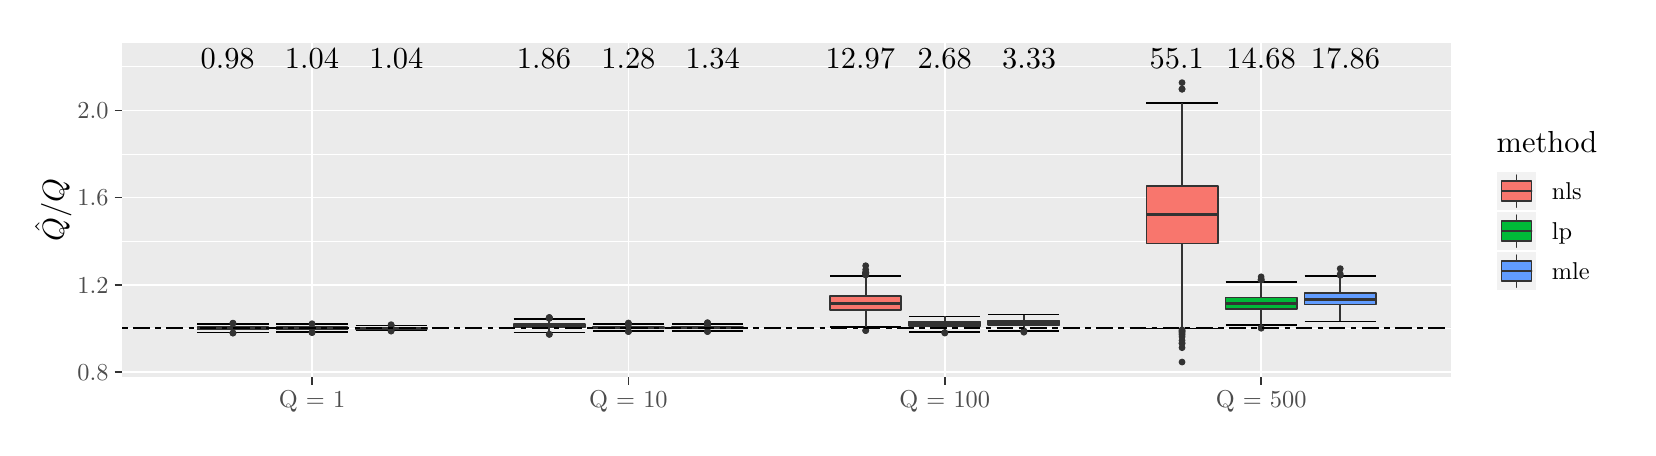
\begin{tikzpicture}[x=1pt,y=1pt]
\definecolor{fillColor}{RGB}{255,255,255}
\path[use as bounding box,fill=fillColor,fill opacity=0.00] (0,0) rectangle (578.16,144.54);
\begin{scope}
\path[clip] (  0.00,  0.00) rectangle (578.16,144.54);
\definecolor{drawColor}{RGB}{255,255,255}
\definecolor{fillColor}{RGB}{255,255,255}

\path[draw=drawColor,line width= 0.6pt,line join=round,line cap=round,fill=fillColor] (  0.00,  0.00) rectangle (578.16,144.54);
\end{scope}
\begin{scope}
\path[clip] ( 34.16, 18.22) rectangle (514.31,139.04);
\definecolor{fillColor}{gray}{0.92}

\path[fill=fillColor] ( 34.16, 18.22) rectangle (514.31,139.04);
\definecolor{drawColor}{RGB}{255,255,255}

\path[draw=drawColor,line width= 0.3pt,line join=round] ( 34.16, 35.91) --
	(514.31, 35.91);

\path[draw=drawColor,line width= 0.3pt,line join=round] ( 34.16, 67.40) --
	(514.31, 67.40);

\path[draw=drawColor,line width= 0.3pt,line join=round] ( 34.16, 98.89) --
	(514.31, 98.89);

\path[draw=drawColor,line width= 0.3pt,line join=round] ( 34.16,130.39) --
	(514.31,130.39);

\path[draw=drawColor,line width= 0.6pt,line join=round] ( 34.16, 20.16) --
	(514.31, 20.16);

\path[draw=drawColor,line width= 0.6pt,line join=round] ( 34.16, 51.65) --
	(514.31, 51.65);

\path[draw=drawColor,line width= 0.6pt,line join=round] ( 34.16, 83.15) --
	(514.31, 83.15);

\path[draw=drawColor,line width= 0.6pt,line join=round] ( 34.16,114.64) --
	(514.31,114.64);

\path[draw=drawColor,line width= 0.6pt,line join=round] (102.75, 18.22) --
	(102.75,139.04);

\path[draw=drawColor,line width= 0.6pt,line join=round] (217.07, 18.22) --
	(217.07,139.04);

\path[draw=drawColor,line width= 0.6pt,line join=round] (331.39, 18.22) --
	(331.39,139.04);

\path[draw=drawColor,line width= 0.6pt,line join=round] (445.71, 18.22) --
	(445.71,139.04);
\definecolor{drawColor}{RGB}{0,0,0}

\path[draw=drawColor,line width= 0.6pt,line join=round] ( 61.31, 37.57) --
	( 87.03, 37.57);

\path[draw=drawColor,line width= 0.6pt,line join=round] ( 74.17, 37.57) --
	( 74.17, 34.35);

\path[draw=drawColor,line width= 0.6pt,line join=round] ( 61.31, 34.35) --
	( 87.03, 34.35);

\path[draw=drawColor,line width= 0.6pt,line join=round] ( 89.89, 37.43) --
	(115.61, 37.43);

\path[draw=drawColor,line width= 0.6pt,line join=round] (102.75, 37.43) --
	(102.75, 34.47);

\path[draw=drawColor,line width= 0.6pt,line join=round] ( 89.89, 34.47) --
	(115.61, 34.47);

\path[draw=drawColor,line width= 0.6pt,line join=round] (118.47, 36.86) --
	(144.19, 36.86);

\path[draw=drawColor,line width= 0.6pt,line join=round] (131.33, 36.86) --
	(131.33, 35.09);

\path[draw=drawColor,line width= 0.6pt,line join=round] (118.47, 35.09) --
	(144.19, 35.09);

\path[draw=drawColor,line width= 0.6pt,line join=round] (175.63, 39.30) --
	(201.35, 39.30);

\path[draw=drawColor,line width= 0.6pt,line join=round] (188.49, 39.30) --
	(188.49, 34.37);

\path[draw=drawColor,line width= 0.6pt,line join=round] (175.63, 34.37) --
	(201.35, 34.37);

\path[draw=drawColor,line width= 0.6pt,line join=round] (204.21, 37.43) --
	(229.93, 37.43);

\path[draw=drawColor,line width= 0.6pt,line join=round] (217.07, 37.43) --
	(217.07, 34.92);

\path[draw=drawColor,line width= 0.6pt,line join=round] (204.21, 34.92) --
	(229.93, 34.92);

\path[draw=drawColor,line width= 0.6pt,line join=round] (232.79, 37.42) --
	(258.51, 37.42);

\path[draw=drawColor,line width= 0.6pt,line join=round] (245.65, 37.42) --
	(245.65, 34.96);

\path[draw=drawColor,line width= 0.6pt,line join=round] (232.79, 34.96) --
	(258.51, 34.96);

\path[draw=drawColor,line width= 0.6pt,line join=round] (289.95, 54.74) --
	(315.67, 54.74);

\path[draw=drawColor,line width= 0.6pt,line join=round] (302.81, 54.74) --
	(302.81, 36.48);

\path[draw=drawColor,line width= 0.6pt,line join=round] (289.95, 36.48) --
	(315.67, 36.48);

\path[draw=drawColor,line width= 0.6pt,line join=round] (318.53, 40.18) --
	(344.25, 40.18);

\path[draw=drawColor,line width= 0.6pt,line join=round] (331.39, 40.18) --
	(331.39, 34.53);

\path[draw=drawColor,line width= 0.6pt,line join=round] (318.53, 34.53) --
	(344.25, 34.53);

\path[draw=drawColor,line width= 0.6pt,line join=round] (347.11, 40.84) --
	(372.83, 40.84);

\path[draw=drawColor,line width= 0.6pt,line join=round] (359.97, 40.84) --
	(359.97, 35.04);

\path[draw=drawColor,line width= 0.6pt,line join=round] (347.11, 35.04) --
	(372.83, 35.04);

\path[draw=drawColor,line width= 0.6pt,line join=round] (404.27,117.30) --
	(430.00,117.30);

\path[draw=drawColor,line width= 0.6pt,line join=round] (417.13,117.30) --
	(417.13, 35.85);

\path[draw=drawColor,line width= 0.6pt,line join=round] (404.27, 35.85) --
	(430.00, 35.85);

\path[draw=drawColor,line width= 0.6pt,line join=round] (432.85, 52.65) --
	(458.58, 52.65);

\path[draw=drawColor,line width= 0.6pt,line join=round] (445.71, 52.65) --
	(445.71, 37.17);

\path[draw=drawColor,line width= 0.6pt,line join=round] (432.85, 37.17) --
	(458.58, 37.17);

\path[draw=drawColor,line width= 0.6pt,line join=round] (461.43, 54.77) --
	(487.16, 54.77);

\path[draw=drawColor,line width= 0.6pt,line join=round] (474.29, 54.77) --
	(474.29, 38.41);

\path[draw=drawColor,line width= 0.6pt,line join=round] (461.43, 38.41) --
	(487.16, 38.41);
\definecolor{drawColor}{gray}{0.20}
\definecolor{fillColor}{gray}{0.20}

\path[draw=drawColor,line width= 0.4pt,line join=round,line cap=round,fill=fillColor] ( 74.17, 37.77) circle (  1.02);

\path[draw=drawColor,line width= 0.4pt,line join=round,line cap=round,fill=fillColor] ( 74.17, 34.19) circle (  1.02);

\path[draw=drawColor,line width= 0.4pt,line join=round,line cap=round,fill=fillColor] ( 74.17, 34.19) circle (  1.02);

\path[draw=drawColor,line width= 0.4pt,line join=round,line cap=round,fill=fillColor] ( 74.17, 37.71) circle (  1.02);

\path[draw=drawColor,line width= 0.6pt,line join=round] ( 74.17, 36.32) -- ( 74.17, 37.57);

\path[draw=drawColor,line width= 0.6pt,line join=round] ( 74.17, 35.48) -- ( 74.17, 34.35);
\definecolor{fillColor}{RGB}{248,118,109}

\path[draw=drawColor,line width= 0.6pt,line join=round,line cap=round,fill=fillColor] ( 61.31, 36.32) --
	( 61.31, 35.48) --
	( 87.03, 35.48) --
	( 87.03, 36.32) --
	( 61.31, 36.32) --
	cycle;

\path[draw=drawColor,line width= 1.1pt,line join=round] ( 61.31, 35.88) -- ( 87.03, 35.88);
\definecolor{fillColor}{gray}{0.20}

\path[draw=drawColor,line width= 0.4pt,line join=round,line cap=round,fill=fillColor] (102.75, 34.39) circle (  1.02);

\path[draw=drawColor,line width= 0.4pt,line join=round,line cap=round,fill=fillColor] (102.75, 37.56) circle (  1.02);

\path[draw=drawColor,line width= 0.4pt,line join=round,line cap=round,fill=fillColor] (102.75, 34.37) circle (  1.02);

\path[draw=drawColor,line width= 0.6pt,line join=round] (102.75, 36.33) -- (102.75, 37.43);

\path[draw=drawColor,line width= 0.6pt,line join=round] (102.75, 35.58) -- (102.75, 34.47);
\definecolor{fillColor}{RGB}{0,186,56}

\path[draw=drawColor,line width= 0.6pt,line join=round,line cap=round,fill=fillColor] ( 89.89, 36.33) --
	( 89.89, 35.58) --
	(115.61, 35.58) --
	(115.61, 36.33) --
	( 89.89, 36.33) --
	cycle;

\path[draw=drawColor,line width= 1.1pt,line join=round] ( 89.89, 35.95) -- (115.61, 35.95);
\definecolor{fillColor}{gray}{0.20}

\path[draw=drawColor,line width= 0.4pt,line join=round,line cap=round,fill=fillColor] (131.33, 34.99) circle (  1.02);

\path[draw=drawColor,line width= 0.4pt,line join=round,line cap=round,fill=fillColor] (131.33, 36.91) circle (  1.02);

\path[draw=drawColor,line width= 0.4pt,line join=round,line cap=round,fill=fillColor] (131.33, 36.95) circle (  1.02);

\path[draw=drawColor,line width= 0.4pt,line join=round,line cap=round,fill=fillColor] (131.33, 37.22) circle (  1.02);

\path[draw=drawColor,line width= 0.4pt,line join=round,line cap=round,fill=fillColor] (131.33, 36.92) circle (  1.02);

\path[draw=drawColor,line width= 0.4pt,line join=round,line cap=round,fill=fillColor] (131.33, 34.90) circle (  1.02);

\path[draw=drawColor,line width= 0.6pt,line join=round] (131.33, 36.19) -- (131.33, 36.86);

\path[draw=drawColor,line width= 0.6pt,line join=round] (131.33, 35.74) -- (131.33, 35.09);
\definecolor{fillColor}{RGB}{97,156,255}

\path[draw=drawColor,line width= 0.6pt,line join=round,line cap=round,fill=fillColor] (118.47, 36.19) --
	(118.47, 35.74) --
	(144.19, 35.74) --
	(144.19, 36.19) --
	(118.47, 36.19) --
	cycle;

\path[draw=drawColor,line width= 1.1pt,line join=round] (118.47, 35.94) -- (144.19, 35.94);
\definecolor{fillColor}{gray}{0.20}

\path[draw=drawColor,line width= 0.4pt,line join=round,line cap=round,fill=fillColor] (188.49, 39.56) circle (  1.02);

\path[draw=drawColor,line width= 0.4pt,line join=round,line cap=round,fill=fillColor] (188.49, 33.73) circle (  1.02);

\path[draw=drawColor,line width= 0.4pt,line join=round,line cap=round,fill=fillColor] (188.49, 39.59) circle (  1.02);

\path[draw=drawColor,line width= 0.4pt,line join=round,line cap=round,fill=fillColor] (188.49, 39.77) circle (  1.02);

\path[draw=drawColor,line width= 0.4pt,line join=round,line cap=round,fill=fillColor] (188.49, 39.53) circle (  1.02);

\path[draw=drawColor,line width= 0.4pt,line join=round,line cap=round,fill=fillColor] (188.49, 33.72) circle (  1.02);

\path[draw=drawColor,line width= 0.4pt,line join=round,line cap=round,fill=fillColor] (188.49, 39.81) circle (  1.02);

\path[draw=drawColor,line width= 0.4pt,line join=round,line cap=round,fill=fillColor] (188.49, 39.70) circle (  1.02);

\path[draw=drawColor,line width= 0.6pt,line join=round] (188.49, 37.45) -- (188.49, 39.30);

\path[draw=drawColor,line width= 0.6pt,line join=round] (188.49, 36.18) -- (188.49, 34.37);
\definecolor{fillColor}{RGB}{248,118,109}

\path[draw=drawColor,line width= 0.6pt,line join=round,line cap=round,fill=fillColor] (175.63, 37.45) --
	(175.63, 36.18) --
	(201.35, 36.18) --
	(201.35, 37.45) --
	(175.63, 37.45) --
	cycle;

\path[draw=drawColor,line width= 1.1pt,line join=round] (175.63, 36.82) -- (201.35, 36.82);
\definecolor{fillColor}{gray}{0.20}

\path[draw=drawColor,line width= 0.4pt,line join=round,line cap=round,fill=fillColor] (217.07, 34.76) circle (  1.02);

\path[draw=drawColor,line width= 0.4pt,line join=round,line cap=round,fill=fillColor] (217.07, 37.43) circle (  1.02);

\path[draw=drawColor,line width= 0.4pt,line join=round,line cap=round,fill=fillColor] (217.07, 34.78) circle (  1.02);

\path[draw=drawColor,line width= 0.4pt,line join=round,line cap=round,fill=fillColor] (217.07, 37.56) circle (  1.02);

\path[draw=drawColor,line width= 0.4pt,line join=round,line cap=round,fill=fillColor] (217.07, 34.77) circle (  1.02);

\path[draw=drawColor,line width= 0.4pt,line join=round,line cap=round,fill=fillColor] (217.07, 37.47) circle (  1.02);

\path[draw=drawColor,line width= 0.4pt,line join=round,line cap=round,fill=fillColor] (217.07, 37.82) circle (  1.02);

\path[draw=drawColor,line width= 0.4pt,line join=round,line cap=round,fill=fillColor] (217.07, 37.52) circle (  1.02);

\path[draw=drawColor,line width= 0.6pt,line join=round] (217.07, 36.44) -- (217.07, 37.43);

\path[draw=drawColor,line width= 0.6pt,line join=round] (217.07, 35.78) -- (217.07, 34.92);
\definecolor{fillColor}{RGB}{0,186,56}

\path[draw=drawColor,line width= 0.6pt,line join=round,line cap=round,fill=fillColor] (204.21, 36.44) --
	(204.21, 35.78) --
	(229.93, 35.78) --
	(229.93, 36.44) --
	(204.21, 36.44) --
	cycle;

\path[draw=drawColor,line width= 1.1pt,line join=round] (204.21, 36.12) -- (229.93, 36.12);
\definecolor{fillColor}{gray}{0.20}

\path[draw=drawColor,line width= 0.4pt,line join=round,line cap=round,fill=fillColor] (245.65, 34.73) circle (  1.02);

\path[draw=drawColor,line width= 0.4pt,line join=round,line cap=round,fill=fillColor] (245.65, 37.44) circle (  1.02);

\path[draw=drawColor,line width= 0.4pt,line join=round,line cap=round,fill=fillColor] (245.65, 34.80) circle (  1.02);

\path[draw=drawColor,line width= 0.4pt,line join=round,line cap=round,fill=fillColor] (245.65, 37.79) circle (  1.02);

\path[draw=drawColor,line width= 0.4pt,line join=round,line cap=round,fill=fillColor] (245.65, 34.83) circle (  1.02);

\path[draw=drawColor,line width= 0.4pt,line join=round,line cap=round,fill=fillColor] (245.65, 37.51) circle (  1.02);

\path[draw=drawColor,line width= 0.4pt,line join=round,line cap=round,fill=fillColor] (245.65, 37.95) circle (  1.02);

\path[draw=drawColor,line width= 0.4pt,line join=round,line cap=round,fill=fillColor] (245.65, 37.49) circle (  1.02);

\path[draw=drawColor,line width= 0.4pt,line join=round,line cap=round,fill=fillColor] (245.65, 37.45) circle (  1.02);

\path[draw=drawColor,line width= 0.4pt,line join=round,line cap=round,fill=fillColor] (245.65, 37.43) circle (  1.02);

\path[draw=drawColor,line width= 0.4pt,line join=round,line cap=round,fill=fillColor] (245.65, 37.76) circle (  1.02);

\path[draw=drawColor,line width= 0.4pt,line join=round,line cap=round,fill=fillColor] (245.65, 37.59) circle (  1.02);

\path[draw=drawColor,line width= 0.6pt,line join=round] (245.65, 36.48) -- (245.65, 37.42);

\path[draw=drawColor,line width= 0.6pt,line join=round] (245.65, 35.86) -- (245.65, 34.96);
\definecolor{fillColor}{RGB}{97,156,255}

\path[draw=drawColor,line width= 0.6pt,line join=round,line cap=round,fill=fillColor] (232.79, 36.48) --
	(232.79, 35.86) --
	(258.51, 35.86) --
	(258.51, 36.48) --
	(232.79, 36.48) --
	cycle;

\path[draw=drawColor,line width= 1.1pt,line join=round] (232.79, 36.17) -- (258.51, 36.17);
\definecolor{fillColor}{gray}{0.20}

\path[draw=drawColor,line width= 0.4pt,line join=round,line cap=round,fill=fillColor] (302.81, 56.00) circle (  1.02);

\path[draw=drawColor,line width= 0.4pt,line join=round,line cap=round,fill=fillColor] (302.81, 35.13) circle (  1.02);

\path[draw=drawColor,line width= 0.4pt,line join=round,line cap=round,fill=fillColor] (302.81, 57.11) circle (  1.02);

\path[draw=drawColor,line width= 0.4pt,line join=round,line cap=round,fill=fillColor] (302.81, 55.72) circle (  1.02);

\path[draw=drawColor,line width= 0.4pt,line join=round,line cap=round,fill=fillColor] (302.81, 55.51) circle (  1.02);

\path[draw=drawColor,line width= 0.4pt,line join=round,line cap=round,fill=fillColor] (302.81, 58.53) circle (  1.02);

\path[draw=drawColor,line width= 0.4pt,line join=round,line cap=round,fill=fillColor] (302.81, 56.07) circle (  1.02);

\path[draw=drawColor,line width= 0.4pt,line join=round,line cap=round,fill=fillColor] (302.81, 55.81) circle (  1.02);

\path[draw=drawColor,line width= 0.4pt,line join=round,line cap=round,fill=fillColor] (302.81, 56.07) circle (  1.02);

\path[draw=drawColor,line width= 0.4pt,line join=round,line cap=round,fill=fillColor] (302.81, 55.16) circle (  1.02);

\path[draw=drawColor,line width= 0.4pt,line join=round,line cap=round,fill=fillColor] (302.81, 35.07) circle (  1.02);

\path[draw=drawColor,line width= 0.6pt,line join=round] (302.81, 47.51) -- (302.81, 54.74);

\path[draw=drawColor,line width= 0.6pt,line join=round] (302.81, 42.56) -- (302.81, 36.48);
\definecolor{fillColor}{RGB}{248,118,109}

\path[draw=drawColor,line width= 0.6pt,line join=round,line cap=round,fill=fillColor] (289.95, 47.51) --
	(289.95, 42.56) --
	(315.67, 42.56) --
	(315.67, 47.51) --
	(289.95, 47.51) --
	cycle;

\path[draw=drawColor,line width= 1.1pt,line join=round] (289.95, 44.96) -- (315.67, 44.96);
\definecolor{fillColor}{gray}{0.20}

\path[draw=drawColor,line width= 0.4pt,line join=round,line cap=round,fill=fillColor] (331.39, 34.19) circle (  1.02);

\path[draw=drawColor,line width= 0.4pt,line join=round,line cap=round,fill=fillColor] (331.39, 34.39) circle (  1.02);

\path[draw=drawColor,line width= 0.6pt,line join=round] (331.39, 38.33) -- (331.39, 40.18);

\path[draw=drawColor,line width= 0.6pt,line join=round] (331.39, 36.78) -- (331.39, 34.53);
\definecolor{fillColor}{RGB}{0,186,56}

\path[draw=drawColor,line width= 0.6pt,line join=round,line cap=round,fill=fillColor] (318.53, 38.33) --
	(318.53, 36.78) --
	(344.25, 36.78) --
	(344.25, 38.33) --
	(318.53, 38.33) --
	cycle;

\path[draw=drawColor,line width= 1.1pt,line join=round] (318.53, 37.59) -- (344.25, 37.59);
\definecolor{fillColor}{gray}{0.20}

\path[draw=drawColor,line width= 0.4pt,line join=round,line cap=round,fill=fillColor] (359.97, 34.50) circle (  1.02);

\path[draw=drawColor,line width= 0.4pt,line join=round,line cap=round,fill=fillColor] (359.97, 34.81) circle (  1.02);

\path[draw=drawColor,line width= 0.4pt,line join=round,line cap=round,fill=fillColor] (359.97, 34.86) circle (  1.02);

\path[draw=drawColor,line width= 0.4pt,line join=round,line cap=round,fill=fillColor] (359.97, 34.82) circle (  1.02);

\path[draw=drawColor,line width= 0.4pt,line join=round,line cap=round,fill=fillColor] (359.97, 34.97) circle (  1.02);

\path[draw=drawColor,line width= 0.6pt,line join=round] (359.97, 38.68) -- (359.97, 40.84);

\path[draw=drawColor,line width= 0.6pt,line join=round] (359.97, 37.20) -- (359.97, 35.04);
\definecolor{fillColor}{RGB}{97,156,255}

\path[draw=drawColor,line width= 0.6pt,line join=round,line cap=round,fill=fillColor] (347.11, 38.68) --
	(347.11, 37.20) --
	(372.83, 37.20) --
	(372.83, 38.68) --
	(347.11, 38.68) --
	cycle;

\path[draw=drawColor,line width= 1.1pt,line join=round] (347.11, 37.96) -- (372.83, 37.96);
\definecolor{fillColor}{gray}{0.20}

\path[draw=drawColor,line width= 0.4pt,line join=round,line cap=round,fill=fillColor] (417.13, 32.84) circle (  1.02);

\path[draw=drawColor,line width= 0.4pt,line join=round,line cap=round,fill=fillColor] (417.13, 23.71) circle (  1.02);

\path[draw=drawColor,line width= 0.4pt,line join=round,line cap=round,fill=fillColor] (417.13, 35.04) circle (  1.02);

\path[draw=drawColor,line width= 0.4pt,line join=round,line cap=round,fill=fillColor] (417.13,122.28) circle (  1.02);

\path[draw=drawColor,line width= 0.4pt,line join=round,line cap=round,fill=fillColor] (417.13, 30.55) circle (  1.02);

\path[draw=drawColor,line width= 0.4pt,line join=round,line cap=round,fill=fillColor] (417.13,122.40) circle (  1.02);

\path[draw=drawColor,line width= 0.4pt,line join=round,line cap=round,fill=fillColor] (417.13, 35.35) circle (  1.02);

\path[draw=drawColor,line width= 0.4pt,line join=round,line cap=round,fill=fillColor] (417.13, 31.52) circle (  1.02);

\path[draw=drawColor,line width= 0.4pt,line join=round,line cap=round,fill=fillColor] (417.13, 33.92) circle (  1.02);

\path[draw=drawColor,line width= 0.4pt,line join=round,line cap=round,fill=fillColor] (417.13, 33.54) circle (  1.02);

\path[draw=drawColor,line width= 0.4pt,line join=round,line cap=round,fill=fillColor] (417.13, 34.44) circle (  1.02);

\path[draw=drawColor,line width= 0.4pt,line join=round,line cap=round,fill=fillColor] (417.13, 30.44) circle (  1.02);

\path[draw=drawColor,line width= 0.4pt,line join=round,line cap=round,fill=fillColor] (417.13,124.67) circle (  1.02);

\path[draw=drawColor,line width= 0.4pt,line join=round,line cap=round,fill=fillColor] (417.13, 34.79) circle (  1.02);

\path[draw=drawColor,line width= 0.4pt,line join=round,line cap=round,fill=fillColor] (417.13, 28.90) circle (  1.02);

\path[draw=drawColor,line width= 0.6pt,line join=round] (417.13, 87.35) -- (417.13,117.30);

\path[draw=drawColor,line width= 0.6pt,line join=round] (417.13, 66.60) -- (417.13, 35.85);
\definecolor{fillColor}{RGB}{248,118,109}

\path[draw=drawColor,line width= 0.6pt,line join=round,line cap=round,fill=fillColor] (404.27, 87.35) --
	(404.27, 66.60) --
	(430.00, 66.60) --
	(430.00, 87.35) --
	(404.27, 87.35) --
	cycle;

\path[draw=drawColor,line width= 1.1pt,line join=round] (404.27, 76.94) -- (430.00, 76.94);
\definecolor{fillColor}{gray}{0.20}

\path[draw=drawColor,line width= 0.4pt,line join=round,line cap=round,fill=fillColor] (445.71, 35.93) circle (  1.02);

\path[draw=drawColor,line width= 0.4pt,line join=round,line cap=round,fill=fillColor] (445.71, 36.14) circle (  1.02);

\path[draw=drawColor,line width= 0.4pt,line join=round,line cap=round,fill=fillColor] (445.71, 53.35) circle (  1.02);

\path[draw=drawColor,line width= 0.4pt,line join=round,line cap=round,fill=fillColor] (445.71, 53.66) circle (  1.02);

\path[draw=drawColor,line width= 0.4pt,line join=round,line cap=round,fill=fillColor] (445.71, 53.35) circle (  1.02);

\path[draw=drawColor,line width= 0.4pt,line join=round,line cap=round,fill=fillColor] (445.71, 54.51) circle (  1.02);

\path[draw=drawColor,line width= 0.4pt,line join=round,line cap=round,fill=fillColor] (445.71, 53.45) circle (  1.02);

\path[draw=drawColor,line width= 0.6pt,line join=round] (445.71, 46.99) -- (445.71, 52.65);

\path[draw=drawColor,line width= 0.6pt,line join=round] (445.71, 42.81) -- (445.71, 37.17);
\definecolor{fillColor}{RGB}{0,186,56}

\path[draw=drawColor,line width= 0.6pt,line join=round,line cap=round,fill=fillColor] (432.85, 46.99) --
	(432.85, 42.81) --
	(458.58, 42.81) --
	(458.58, 46.99) --
	(432.85, 46.99) --
	cycle;

\path[draw=drawColor,line width= 1.1pt,line join=round] (432.85, 44.96) -- (458.58, 44.96);
\definecolor{fillColor}{gray}{0.20}

\path[draw=drawColor,line width= 0.4pt,line join=round,line cap=round,fill=fillColor] (474.29, 57.47) circle (  1.02);

\path[draw=drawColor,line width= 0.4pt,line join=round,line cap=round,fill=fillColor] (474.29, 55.06) circle (  1.02);

\path[draw=drawColor,line width= 0.4pt,line join=round,line cap=round,fill=fillColor] (474.29, 55.56) circle (  1.02);

\path[draw=drawColor,line width= 0.6pt,line join=round] (474.29, 48.60) -- (474.29, 54.77);

\path[draw=drawColor,line width= 0.6pt,line join=round] (474.29, 44.46) -- (474.29, 38.41);
\definecolor{fillColor}{RGB}{97,156,255}

\path[draw=drawColor,line width= 0.6pt,line join=round,line cap=round,fill=fillColor] (461.43, 48.60) --
	(461.43, 44.46) --
	(487.16, 44.46) --
	(487.16, 48.60) --
	(461.43, 48.60) --
	cycle;

\path[draw=drawColor,line width= 1.1pt,line join=round] (461.43, 46.40) -- (487.16, 46.40);
\definecolor{drawColor}{RGB}{0,0,0}

\path[draw=drawColor,line width= 0.6pt,dash pattern=on 2pt off 2pt on 6pt off 2pt ,line join=round] ( 34.16, 35.91) -- (514.31, 35.91);

\node[text=drawColor,anchor=base,inner sep=0pt, outer sep=0pt, scale=  1.10] at (133.23,129.75) {1.04};

\node[text=drawColor,anchor=base,inner sep=0pt, outer sep=0pt, scale=  1.10] at (102.75,129.75) {1.04};

\node[text=drawColor,anchor=base,inner sep=0pt, outer sep=0pt, scale=  1.10] at ( 72.26,129.75) {0.98};

\node[text=drawColor,anchor=base,inner sep=0pt, outer sep=0pt, scale=  1.10] at (247.56,129.75) {1.34};

\node[text=drawColor,anchor=base,inner sep=0pt, outer sep=0pt, scale=  1.10] at (217.07,129.75) {1.28};

\node[text=drawColor,anchor=base,inner sep=0pt, outer sep=0pt, scale=  1.10] at (186.59,129.75) {1.86};

\node[text=drawColor,anchor=base,inner sep=0pt, outer sep=0pt, scale=  1.10] at (361.88,129.75) {3.33};

\node[text=drawColor,anchor=base,inner sep=0pt, outer sep=0pt, scale=  1.10] at (331.39,129.75) {2.68};

\node[text=drawColor,anchor=base,inner sep=0pt, outer sep=0pt, scale=  1.10] at (300.91,129.75) {12.97};

\node[text=drawColor,anchor=base,inner sep=0pt, outer sep=0pt, scale=  1.10] at (476.20,129.75) {17.86};

\node[text=drawColor,anchor=base,inner sep=0pt, outer sep=0pt, scale=  1.10] at (445.71,129.75) {14.68};

\node[text=drawColor,anchor=base,inner sep=0pt, outer sep=0pt, scale=  1.10] at (415.23,129.75) {55.1};
\end{scope}
\begin{scope}
\path[clip] (  0.00,  0.00) rectangle (578.16,144.54);
\definecolor{drawColor}{gray}{0.30}

\node[text=drawColor,anchor=base east,inner sep=0pt, outer sep=0pt, scale=  0.88] at ( 29.21, 17.13) {0.8};

\node[text=drawColor,anchor=base east,inner sep=0pt, outer sep=0pt, scale=  0.88] at ( 29.21, 48.62) {1.2};

\node[text=drawColor,anchor=base east,inner sep=0pt, outer sep=0pt, scale=  0.88] at ( 29.21, 80.12) {1.6};

\node[text=drawColor,anchor=base east,inner sep=0pt, outer sep=0pt, scale=  0.88] at ( 29.21,111.61) {2.0};
\end{scope}
\begin{scope}
\path[clip] (  0.00,  0.00) rectangle (578.16,144.54);
\definecolor{drawColor}{gray}{0.20}

\path[draw=drawColor,line width= 0.6pt,line join=round] ( 31.41, 20.16) --
	( 34.16, 20.16);

\path[draw=drawColor,line width= 0.6pt,line join=round] ( 31.41, 51.65) --
	( 34.16, 51.65);

\path[draw=drawColor,line width= 0.6pt,line join=round] ( 31.41, 83.15) --
	( 34.16, 83.15);

\path[draw=drawColor,line width= 0.6pt,line join=round] ( 31.41,114.64) --
	( 34.16,114.64);
\end{scope}
\begin{scope}
\path[clip] (  0.00,  0.00) rectangle (578.16,144.54);
\definecolor{drawColor}{gray}{0.20}

\path[draw=drawColor,line width= 0.6pt,line join=round] (102.75, 15.47) --
	(102.75, 18.22);

\path[draw=drawColor,line width= 0.6pt,line join=round] (217.07, 15.47) --
	(217.07, 18.22);

\path[draw=drawColor,line width= 0.6pt,line join=round] (331.39, 15.47) --
	(331.39, 18.22);

\path[draw=drawColor,line width= 0.6pt,line join=round] (445.71, 15.47) --
	(445.71, 18.22);
\end{scope}
\begin{scope}
\path[clip] (  0.00,  0.00) rectangle (578.16,144.54);
\definecolor{drawColor}{gray}{0.30}

\node[text=drawColor,anchor=base,inner sep=0pt, outer sep=0pt, scale=  0.88] at (102.75,  7.21) {Q = 1};

\node[text=drawColor,anchor=base,inner sep=0pt, outer sep=0pt, scale=  0.88] at (217.07,  7.21) {Q = 10};

\node[text=drawColor,anchor=base,inner sep=0pt, outer sep=0pt, scale=  0.88] at (331.39,  7.21) {Q = 100};

\node[text=drawColor,anchor=base,inner sep=0pt, outer sep=0pt, scale=  0.88] at (445.71,  7.21) {Q = 500};
\end{scope}
\begin{scope}
\path[clip] (  0.00,  0.00) rectangle (578.16,144.54);
\definecolor{drawColor}{RGB}{0,0,0}

\node[text=drawColor,rotate= 90.00,anchor=base,inner sep=0pt, outer sep=0pt, scale=  1.10] at ( 13.08, 78.63) {$\hat{Q}/Q$};
\end{scope}
\begin{scope}
\path[clip] (  0.00,  0.00) rectangle (578.16,144.54);
\definecolor{fillColor}{RGB}{255,255,255}

\path[fill=fillColor] (525.31, 43.84) rectangle (572.66,113.42);
\end{scope}
\begin{scope}
\path[clip] (  0.00,  0.00) rectangle (578.16,144.54);
\definecolor{drawColor}{RGB}{0,0,0}

\node[text=drawColor,anchor=base west,inner sep=0pt, outer sep=0pt, scale=  1.10] at (530.81, 99.27) {method};
\end{scope}
\begin{scope}
\path[clip] (  0.00,  0.00) rectangle (578.16,144.54);
\definecolor{drawColor}{RGB}{255,255,255}
\definecolor{fillColor}{gray}{0.95}

\path[draw=drawColor,line width= 0.6pt,line join=round,line cap=round,fill=fillColor] (530.81, 78.25) rectangle (545.26, 92.70);
\end{scope}
\begin{scope}
\path[clip] (  0.00,  0.00) rectangle (578.16,144.54);
\definecolor{drawColor}{gray}{0.20}

\path[draw=drawColor,line width= 0.6pt,line join=round,line cap=round] (538.03, 79.70) --
	(538.03, 81.86);

\path[draw=drawColor,line width= 0.6pt,line join=round,line cap=round] (538.03, 89.09) --
	(538.03, 91.26);
\definecolor{fillColor}{RGB}{248,118,109}

\path[draw=drawColor,line width= 0.6pt,line join=round,line cap=round,fill=fillColor] (532.61, 81.86) rectangle (543.45, 89.09);

\path[draw=drawColor,line width= 0.6pt,line join=round,line cap=round] (532.61, 85.48) --
	(543.45, 85.48);
\end{scope}
\begin{scope}
\path[clip] (  0.00,  0.00) rectangle (578.16,144.54);
\definecolor{drawColor}{RGB}{255,255,255}
\definecolor{fillColor}{gray}{0.95}

\path[draw=drawColor,line width= 0.6pt,line join=round,line cap=round,fill=fillColor] (530.81, 63.80) rectangle (545.26, 78.25);
\end{scope}
\begin{scope}
\path[clip] (  0.00,  0.00) rectangle (578.16,144.54);
\definecolor{drawColor}{gray}{0.20}

\path[draw=drawColor,line width= 0.6pt,line join=round,line cap=round] (538.03, 65.24) --
	(538.03, 67.41);

\path[draw=drawColor,line width= 0.6pt,line join=round,line cap=round] (538.03, 74.64) --
	(538.03, 76.81);
\definecolor{fillColor}{RGB}{0,186,56}

\path[draw=drawColor,line width= 0.6pt,line join=round,line cap=round,fill=fillColor] (532.61, 67.41) rectangle (543.45, 74.64);

\path[draw=drawColor,line width= 0.6pt,line join=round,line cap=round] (532.61, 71.02) --
	(543.45, 71.02);
\end{scope}
\begin{scope}
\path[clip] (  0.00,  0.00) rectangle (578.16,144.54);
\definecolor{drawColor}{RGB}{255,255,255}
\definecolor{fillColor}{gray}{0.95}

\path[draw=drawColor,line width= 0.6pt,line join=round,line cap=round,fill=fillColor] (530.81, 49.34) rectangle (545.26, 63.80);
\end{scope}
\begin{scope}
\path[clip] (  0.00,  0.00) rectangle (578.16,144.54);
\definecolor{drawColor}{gray}{0.20}

\path[draw=drawColor,line width= 0.6pt,line join=round,line cap=round] (538.03, 50.79) --
	(538.03, 52.96);

\path[draw=drawColor,line width= 0.6pt,line join=round,line cap=round] (538.03, 60.18) --
	(538.03, 62.35);
\definecolor{fillColor}{RGB}{97,156,255}

\path[draw=drawColor,line width= 0.6pt,line join=round,line cap=round,fill=fillColor] (532.61, 52.96) rectangle (543.45, 60.18);

\path[draw=drawColor,line width= 0.6pt,line join=round,line cap=round] (532.61, 56.57) --
	(543.45, 56.57);
\end{scope}
\begin{scope}
\path[clip] (  0.00,  0.00) rectangle (578.16,144.54);
\definecolor{drawColor}{RGB}{0,0,0}

\node[text=drawColor,anchor=base west,inner sep=0pt, outer sep=0pt, scale=  0.88] at (550.76, 82.45) {nls};
\end{scope}
\begin{scope}
\path[clip] (  0.00,  0.00) rectangle (578.16,144.54);
\definecolor{drawColor}{RGB}{0,0,0}

\node[text=drawColor,anchor=base west,inner sep=0pt, outer sep=0pt, scale=  0.88] at (550.76, 67.99) {lp};
\end{scope}
\begin{scope}
\path[clip] (  0.00,  0.00) rectangle (578.16,144.54);
\definecolor{drawColor}{RGB}{0,0,0}

\node[text=drawColor,anchor=base west,inner sep=0pt, outer sep=0pt, scale=  0.88] at (550.76, 53.54) {mle};
\end{scope}
\end{tikzpicture}
}
%   \end{subfigure}
%   \hfill
%   \begin{subfigure}
%     \centering
%     \resizebox{1.1\linewidth}{!}{% Created by tikzDevice version 0.12.3 on 2019-09-28 14:19:35
% !TEX encoding = UTF-8 Unicode
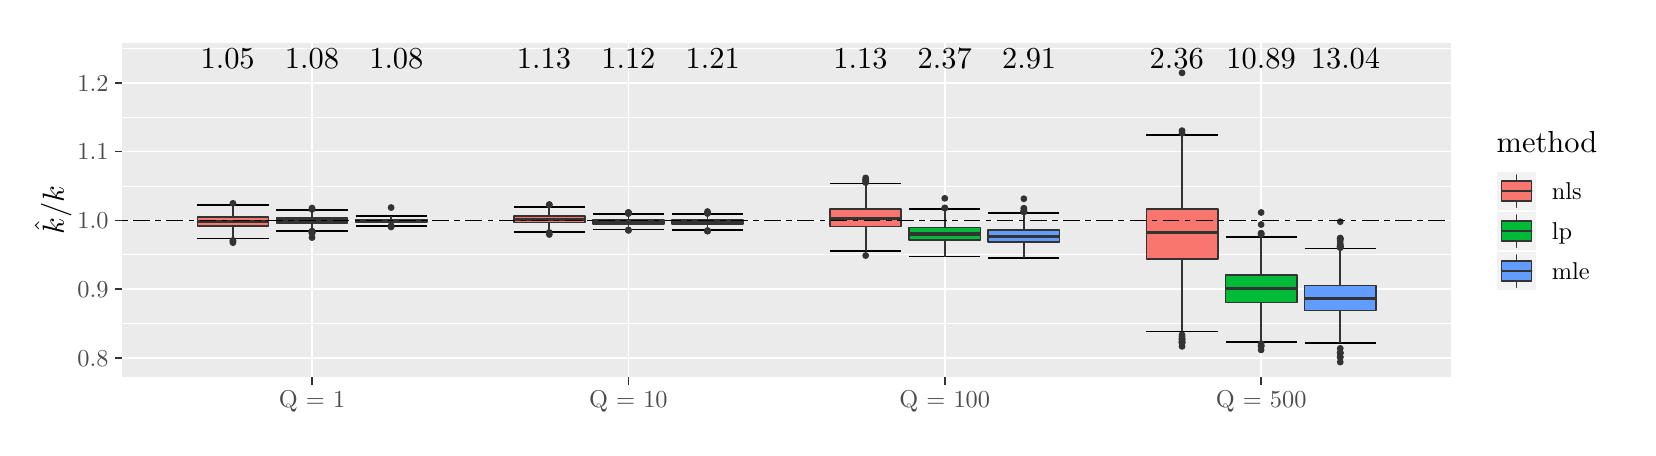
\begin{tikzpicture}[x=1pt,y=1pt]
\definecolor{fillColor}{RGB}{255,255,255}
\path[use as bounding box,fill=fillColor,fill opacity=0.00] (0,0) rectangle (578.16,144.54);
\begin{scope}
\path[clip] (  0.00,  0.00) rectangle (578.16,144.54);
\definecolor{drawColor}{RGB}{255,255,255}
\definecolor{fillColor}{RGB}{255,255,255}

\path[draw=drawColor,line width= 0.6pt,line join=round,line cap=round,fill=fillColor] (  0.00,  0.00) rectangle (578.16,144.54);
\end{scope}
\begin{scope}
\path[clip] ( 34.16, 18.22) rectangle (514.31,139.04);
\definecolor{fillColor}{gray}{0.92}

\path[fill=fillColor] ( 34.16, 18.22) rectangle (514.31,139.04);
\definecolor{drawColor}{RGB}{255,255,255}

\path[draw=drawColor,line width= 0.3pt,line join=round] ( 34.16, 37.56) --
	(514.31, 37.56);

\path[draw=drawColor,line width= 0.3pt,line join=round] ( 34.16, 62.44) --
	(514.31, 62.44);

\path[draw=drawColor,line width= 0.3pt,line join=round] ( 34.16, 87.33) --
	(514.31, 87.33);

\path[draw=drawColor,line width= 0.3pt,line join=round] ( 34.16,112.21) --
	(514.31,112.21);

\path[draw=drawColor,line width= 0.3pt,line join=round] ( 34.16,137.09) --
	(514.31,137.09);

\path[draw=drawColor,line width= 0.6pt,line join=round] ( 34.16, 25.12) --
	(514.31, 25.12);

\path[draw=drawColor,line width= 0.6pt,line join=round] ( 34.16, 50.00) --
	(514.31, 50.00);

\path[draw=drawColor,line width= 0.6pt,line join=round] ( 34.16, 74.88) --
	(514.31, 74.88);

\path[draw=drawColor,line width= 0.6pt,line join=round] ( 34.16, 99.77) --
	(514.31, 99.77);

\path[draw=drawColor,line width= 0.6pt,line join=round] ( 34.16,124.65) --
	(514.31,124.65);

\path[draw=drawColor,line width= 0.6pt,line join=round] (102.75, 18.22) --
	(102.75,139.04);

\path[draw=drawColor,line width= 0.6pt,line join=round] (217.07, 18.22) --
	(217.07,139.04);

\path[draw=drawColor,line width= 0.6pt,line join=round] (331.39, 18.22) --
	(331.39,139.04);

\path[draw=drawColor,line width= 0.6pt,line join=round] (445.71, 18.22) --
	(445.71,139.04);
\definecolor{drawColor}{RGB}{0,0,0}

\path[draw=drawColor,line width= 0.6pt,line join=round] ( 61.31, 80.51) --
	( 87.03, 80.51);

\path[draw=drawColor,line width= 0.6pt,line join=round] ( 74.17, 80.51) --
	( 74.17, 68.34);

\path[draw=drawColor,line width= 0.6pt,line join=round] ( 61.31, 68.34) --
	( 87.03, 68.34);

\path[draw=drawColor,line width= 0.6pt,line join=round] ( 89.89, 78.66) --
	(115.61, 78.66);

\path[draw=drawColor,line width= 0.6pt,line join=round] (102.75, 78.66) --
	(102.75, 71.03);

\path[draw=drawColor,line width= 0.6pt,line join=round] ( 89.89, 71.03) --
	(115.61, 71.03);

\path[draw=drawColor,line width= 0.6pt,line join=round] (118.47, 76.58) --
	(144.19, 76.58);

\path[draw=drawColor,line width= 0.6pt,line join=round] (131.33, 76.58) --
	(131.33, 72.98);

\path[draw=drawColor,line width= 0.6pt,line join=round] (118.47, 72.98) --
	(144.19, 72.98);

\path[draw=drawColor,line width= 0.6pt,line join=round] (175.63, 79.85) --
	(201.35, 79.85);

\path[draw=drawColor,line width= 0.6pt,line join=round] (188.49, 79.85) --
	(188.49, 70.61);

\path[draw=drawColor,line width= 0.6pt,line join=round] (175.63, 70.61) --
	(201.35, 70.61);

\path[draw=drawColor,line width= 0.6pt,line join=round] (204.21, 77.28) --
	(229.93, 77.28);

\path[draw=drawColor,line width= 0.6pt,line join=round] (217.07, 77.28) --
	(217.07, 71.55);

\path[draw=drawColor,line width= 0.6pt,line join=round] (204.21, 71.55) --
	(229.93, 71.55);

\path[draw=drawColor,line width= 0.6pt,line join=round] (232.79, 77.13) --
	(258.51, 77.13);

\path[draw=drawColor,line width= 0.6pt,line join=round] (245.65, 77.13) --
	(245.65, 71.49);

\path[draw=drawColor,line width= 0.6pt,line join=round] (232.79, 71.49) --
	(258.51, 71.49);

\path[draw=drawColor,line width= 0.6pt,line join=round] (289.95, 88.27) --
	(315.67, 88.27);

\path[draw=drawColor,line width= 0.6pt,line join=round] (302.81, 88.27) --
	(302.81, 63.81);

\path[draw=drawColor,line width= 0.6pt,line join=round] (289.95, 63.81) --
	(315.67, 63.81);

\path[draw=drawColor,line width= 0.6pt,line join=round] (318.53, 78.91) --
	(344.25, 78.91);

\path[draw=drawColor,line width= 0.6pt,line join=round] (331.39, 78.91) --
	(331.39, 61.81);

\path[draw=drawColor,line width= 0.6pt,line join=round] (318.53, 61.81) --
	(344.25, 61.81);

\path[draw=drawColor,line width= 0.6pt,line join=round] (347.11, 77.67) --
	(372.83, 77.67);

\path[draw=drawColor,line width= 0.6pt,line join=round] (359.97, 77.67) --
	(359.97, 61.26);

\path[draw=drawColor,line width= 0.6pt,line join=round] (347.11, 61.26) --
	(372.83, 61.26);

\path[draw=drawColor,line width= 0.6pt,line join=round] (404.27,105.71) --
	(430.00,105.71);

\path[draw=drawColor,line width= 0.6pt,line join=round] (417.13,105.71) --
	(417.13, 34.76);

\path[draw=drawColor,line width= 0.6pt,line join=round] (404.27, 34.76) --
	(430.00, 34.76);

\path[draw=drawColor,line width= 0.6pt,line join=round] (432.85, 68.98) --
	(458.58, 68.98);

\path[draw=drawColor,line width= 0.6pt,line join=round] (445.71, 68.98) --
	(445.71, 31.06);

\path[draw=drawColor,line width= 0.6pt,line join=round] (432.85, 31.06) --
	(458.58, 31.06);

\path[draw=drawColor,line width= 0.6pt,line join=round] (461.43, 64.79) --
	(487.16, 64.79);

\path[draw=drawColor,line width= 0.6pt,line join=round] (474.29, 64.79) --
	(474.29, 30.53);

\path[draw=drawColor,line width= 0.6pt,line join=round] (461.43, 30.53) --
	(487.16, 30.53);
\definecolor{drawColor}{gray}{0.20}
\definecolor{fillColor}{gray}{0.20}

\path[draw=drawColor,line width= 0.4pt,line join=round,line cap=round,fill=fillColor] ( 74.17, 66.85) circle (  1.02);

\path[draw=drawColor,line width= 0.4pt,line join=round,line cap=round,fill=fillColor] ( 74.17, 67.69) circle (  1.02);

\path[draw=drawColor,line width= 0.4pt,line join=round,line cap=round,fill=fillColor] ( 74.17, 67.37) circle (  1.02);

\path[draw=drawColor,line width= 0.4pt,line join=round,line cap=round,fill=fillColor] ( 74.17, 81.07) circle (  1.02);

\path[draw=drawColor,line width= 0.6pt,line join=round] ( 74.17, 76.04) -- ( 74.17, 80.51);

\path[draw=drawColor,line width= 0.6pt,line join=round] ( 74.17, 72.89) -- ( 74.17, 68.34);
\definecolor{fillColor}{RGB}{248,118,109}

\path[draw=drawColor,line width= 0.6pt,line join=round,line cap=round,fill=fillColor] ( 61.31, 76.04) --
	( 61.31, 72.89) --
	( 87.03, 72.89) --
	( 87.03, 76.04) --
	( 61.31, 76.04) --
	cycle;

\path[draw=drawColor,line width= 1.1pt,line join=round] ( 61.31, 74.52) -- ( 87.03, 74.52);
\definecolor{fillColor}{gray}{0.20}

\path[draw=drawColor,line width= 0.4pt,line join=round,line cap=round,fill=fillColor] (102.75, 70.39) circle (  1.02);

\path[draw=drawColor,line width= 0.4pt,line join=round,line cap=round,fill=fillColor] (102.75, 79.36) circle (  1.02);

\path[draw=drawColor,line width= 0.4pt,line join=round,line cap=round,fill=fillColor] (102.75, 68.69) circle (  1.02);

\path[draw=drawColor,line width= 0.4pt,line join=round,line cap=round,fill=fillColor] (102.75, 70.66) circle (  1.02);

\path[draw=drawColor,line width= 0.4pt,line join=round,line cap=round,fill=fillColor] (102.75, 70.98) circle (  1.02);

\path[draw=drawColor,line width= 0.4pt,line join=round,line cap=round,fill=fillColor] (102.75, 70.89) circle (  1.02);

\path[draw=drawColor,line width= 0.4pt,line join=round,line cap=round,fill=fillColor] (102.75, 70.82) circle (  1.02);

\path[draw=drawColor,line width= 0.4pt,line join=round,line cap=round,fill=fillColor] (102.75, 70.88) circle (  1.02);

\path[draw=drawColor,line width= 0.4pt,line join=round,line cap=round,fill=fillColor] (102.75, 70.78) circle (  1.02);

\path[draw=drawColor,line width= 0.4pt,line join=round,line cap=round,fill=fillColor] (102.75, 70.83) circle (  1.02);

\path[draw=drawColor,line width= 0.4pt,line join=round,line cap=round,fill=fillColor] (102.75, 70.24) circle (  1.02);

\path[draw=drawColor,line width= 0.4pt,line join=round,line cap=round,fill=fillColor] (102.75, 78.86) circle (  1.02);

\path[draw=drawColor,line width= 0.6pt,line join=round] (102.75, 75.80) -- (102.75, 78.66);

\path[draw=drawColor,line width= 0.6pt,line join=round] (102.75, 73.89) -- (102.75, 71.03);
\definecolor{fillColor}{RGB}{0,186,56}

\path[draw=drawColor,line width= 0.6pt,line join=round,line cap=round,fill=fillColor] ( 89.89, 75.80) --
	( 89.89, 73.89) --
	(115.61, 73.89) --
	(115.61, 75.80) --
	( 89.89, 75.80) --
	cycle;

\path[draw=drawColor,line width= 1.1pt,line join=round] ( 89.89, 74.82) -- (115.61, 74.82);
\definecolor{fillColor}{gray}{0.20}

\path[draw=drawColor,line width= 0.4pt,line join=round,line cap=round,fill=fillColor] (131.33, 72.65) circle (  1.02);

\path[draw=drawColor,line width= 0.4pt,line join=round,line cap=round,fill=fillColor] (131.33, 72.88) circle (  1.02);

\path[draw=drawColor,line width= 0.4pt,line join=round,line cap=round,fill=fillColor] (131.33, 72.54) circle (  1.02);

\path[draw=drawColor,line width= 0.4pt,line join=round,line cap=round,fill=fillColor] (131.33, 79.54) circle (  1.02);

\path[draw=drawColor,line width= 0.4pt,line join=round,line cap=round,fill=fillColor] (131.33, 72.96) circle (  1.02);

\path[draw=drawColor,line width= 0.6pt,line join=round] (131.33, 75.24) -- (131.33, 76.58);

\path[draw=drawColor,line width= 0.6pt,line join=round] (131.33, 74.33) -- (131.33, 72.98);
\definecolor{fillColor}{RGB}{97,156,255}

\path[draw=drawColor,line width= 0.6pt,line join=round,line cap=round,fill=fillColor] (118.47, 75.24) --
	(118.47, 74.33) --
	(144.19, 74.33) --
	(144.19, 75.24) --
	(118.47, 75.24) --
	cycle;

\path[draw=drawColor,line width= 1.1pt,line join=round] (118.47, 74.78) -- (144.19, 74.78);
\definecolor{fillColor}{gray}{0.20}

\path[draw=drawColor,line width= 0.4pt,line join=round,line cap=round,fill=fillColor] (188.49, 80.50) circle (  1.02);

\path[draw=drawColor,line width= 0.4pt,line join=round,line cap=round,fill=fillColor] (188.49, 70.54) circle (  1.02);

\path[draw=drawColor,line width= 0.4pt,line join=round,line cap=round,fill=fillColor] (188.49, 80.64) circle (  1.02);

\path[draw=drawColor,line width= 0.4pt,line join=round,line cap=round,fill=fillColor] (188.49, 69.81) circle (  1.02);

\path[draw=drawColor,line width= 0.6pt,line join=round] (188.49, 76.43) -- (188.49, 79.85);

\path[draw=drawColor,line width= 0.6pt,line join=round] (188.49, 74.08) -- (188.49, 70.61);
\definecolor{fillColor}{RGB}{248,118,109}

\path[draw=drawColor,line width= 0.6pt,line join=round,line cap=round,fill=fillColor] (175.63, 76.43) --
	(175.63, 74.08) --
	(201.35, 74.08) --
	(201.35, 76.43) --
	(175.63, 76.43) --
	cycle;

\path[draw=drawColor,line width= 1.1pt,line join=round] (175.63, 75.23) -- (201.35, 75.23);
\definecolor{fillColor}{gray}{0.20}

\path[draw=drawColor,line width= 0.4pt,line join=round,line cap=round,fill=fillColor] (217.07, 77.53) circle (  1.02);

\path[draw=drawColor,line width= 0.4pt,line join=round,line cap=round,fill=fillColor] (217.07, 71.46) circle (  1.02);

\path[draw=drawColor,line width= 0.4pt,line join=round,line cap=round,fill=fillColor] (217.07, 77.73) circle (  1.02);

\path[draw=drawColor,line width= 0.4pt,line join=round,line cap=round,fill=fillColor] (217.07, 77.68) circle (  1.02);

\path[draw=drawColor,line width= 0.4pt,line join=round,line cap=round,fill=fillColor] (217.07, 77.54) circle (  1.02);

\path[draw=drawColor,line width= 0.4pt,line join=round,line cap=round,fill=fillColor] (217.07, 77.38) circle (  1.02);

\path[draw=drawColor,line width= 0.4pt,line join=round,line cap=round,fill=fillColor] (217.07, 71.32) circle (  1.02);

\path[draw=drawColor,line width= 0.4pt,line join=round,line cap=round,fill=fillColor] (217.07, 77.45) circle (  1.02);

\path[draw=drawColor,line width= 0.4pt,line join=round,line cap=round,fill=fillColor] (217.07, 77.76) circle (  1.02);

\path[draw=drawColor,line width= 0.4pt,line join=round,line cap=round,fill=fillColor] (217.07, 71.33) circle (  1.02);

\path[draw=drawColor,line width= 0.6pt,line join=round] (217.07, 75.14) -- (217.07, 77.28);

\path[draw=drawColor,line width= 0.6pt,line join=round] (217.07, 73.68) -- (217.07, 71.55);
\definecolor{fillColor}{RGB}{0,186,56}

\path[draw=drawColor,line width= 0.6pt,line join=round,line cap=round,fill=fillColor] (204.21, 75.14) --
	(204.21, 73.68) --
	(229.93, 73.68) --
	(229.93, 75.14) --
	(204.21, 75.14) --
	cycle;

\path[draw=drawColor,line width= 1.1pt,line join=round] (204.21, 74.44) -- (229.93, 74.44);
\definecolor{fillColor}{gray}{0.20}

\path[draw=drawColor,line width= 0.4pt,line join=round,line cap=round,fill=fillColor] (245.65, 71.10) circle (  1.02);

\path[draw=drawColor,line width= 0.4pt,line join=round,line cap=round,fill=fillColor] (245.65, 77.47) circle (  1.02);

\path[draw=drawColor,line width= 0.4pt,line join=round,line cap=round,fill=fillColor] (245.65, 71.23) circle (  1.02);

\path[draw=drawColor,line width= 0.4pt,line join=round,line cap=round,fill=fillColor] (245.65, 77.58) circle (  1.02);

\path[draw=drawColor,line width= 0.4pt,line join=round,line cap=round,fill=fillColor] (245.65, 77.42) circle (  1.02);

\path[draw=drawColor,line width= 0.4pt,line join=round,line cap=round,fill=fillColor] (245.65, 71.05) circle (  1.02);

\path[draw=drawColor,line width= 0.4pt,line join=round,line cap=round,fill=fillColor] (245.65, 78.10) circle (  1.02);

\path[draw=drawColor,line width= 0.4pt,line join=round,line cap=round,fill=fillColor] (245.65, 71.09) circle (  1.02);

\path[draw=drawColor,line width= 0.6pt,line join=round] (245.65, 75.01) -- (245.65, 77.13);

\path[draw=drawColor,line width= 0.6pt,line join=round] (245.65, 73.52) -- (245.65, 71.49);
\definecolor{fillColor}{RGB}{97,156,255}

\path[draw=drawColor,line width= 0.6pt,line join=round,line cap=round,fill=fillColor] (232.79, 75.01) --
	(232.79, 73.52) --
	(258.51, 73.52) --
	(258.51, 75.01) --
	(232.79, 75.01) --
	cycle;

\path[draw=drawColor,line width= 1.1pt,line join=round] (232.79, 74.31) -- (258.51, 74.31);
\definecolor{fillColor}{gray}{0.20}

\path[draw=drawColor,line width= 0.4pt,line join=round,line cap=round,fill=fillColor] (302.81, 62.20) circle (  1.02);

\path[draw=drawColor,line width= 0.4pt,line join=round,line cap=round,fill=fillColor] (302.81, 89.63) circle (  1.02);

\path[draw=drawColor,line width= 0.4pt,line join=round,line cap=round,fill=fillColor] (302.81, 88.56) circle (  1.02);

\path[draw=drawColor,line width= 0.4pt,line join=round,line cap=round,fill=fillColor] (302.81, 88.99) circle (  1.02);

\path[draw=drawColor,line width= 0.4pt,line join=round,line cap=round,fill=fillColor] (302.81, 89.39) circle (  1.02);

\path[draw=drawColor,line width= 0.4pt,line join=round,line cap=round,fill=fillColor] (302.81, 90.25) circle (  1.02);

\path[draw=drawColor,line width= 0.6pt,line join=round] (302.81, 78.98) -- (302.81, 88.27);

\path[draw=drawColor,line width= 0.6pt,line join=round] (302.81, 72.73) -- (302.81, 63.81);
\definecolor{fillColor}{RGB}{248,118,109}

\path[draw=drawColor,line width= 0.6pt,line join=round,line cap=round,fill=fillColor] (289.95, 78.98) --
	(289.95, 72.73) --
	(315.67, 72.73) --
	(315.67, 78.98) --
	(289.95, 78.98) --
	cycle;

\path[draw=drawColor,line width= 1.1pt,line join=round] (289.95, 75.68) -- (315.67, 75.68);
\definecolor{fillColor}{gray}{0.20}

\path[draw=drawColor,line width= 0.4pt,line join=round,line cap=round,fill=fillColor] (331.39, 82.87) circle (  1.02);

\path[draw=drawColor,line width= 0.4pt,line join=round,line cap=round,fill=fillColor] (331.39, 79.35) circle (  1.02);

\path[draw=drawColor,line width= 0.4pt,line join=round,line cap=round,fill=fillColor] (331.39, 79.39) circle (  1.02);

\path[draw=drawColor,line width= 0.6pt,line join=round] (331.39, 72.34) -- (331.39, 78.91);

\path[draw=drawColor,line width= 0.6pt,line join=round] (331.39, 67.92) -- (331.39, 61.81);
\definecolor{fillColor}{RGB}{0,186,56}

\path[draw=drawColor,line width= 0.6pt,line join=round,line cap=round,fill=fillColor] (318.53, 72.34) --
	(318.53, 67.92) --
	(344.25, 67.92) --
	(344.25, 72.34) --
	(318.53, 72.34) --
	cycle;

\path[draw=drawColor,line width= 1.1pt,line join=round] (318.53, 69.98) -- (344.25, 69.98);
\definecolor{fillColor}{gray}{0.20}

\path[draw=drawColor,line width= 0.4pt,line join=round,line cap=round,fill=fillColor] (359.97, 77.98) circle (  1.02);

\path[draw=drawColor,line width= 0.4pt,line join=round,line cap=round,fill=fillColor] (359.97, 82.72) circle (  1.02);

\path[draw=drawColor,line width= 0.4pt,line join=round,line cap=round,fill=fillColor] (359.97, 79.20) circle (  1.02);

\path[draw=drawColor,line width= 0.4pt,line join=round,line cap=round,fill=fillColor] (359.97, 79.26) circle (  1.02);

\path[draw=drawColor,line width= 0.4pt,line join=round,line cap=round,fill=fillColor] (359.97, 78.13) circle (  1.02);

\path[draw=drawColor,line width= 0.4pt,line join=round,line cap=round,fill=fillColor] (359.97, 78.34) circle (  1.02);

\path[draw=drawColor,line width= 0.4pt,line join=round,line cap=round,fill=fillColor] (359.97, 78.10) circle (  1.02);

\path[draw=drawColor,line width= 0.4pt,line join=round,line cap=round,fill=fillColor] (359.97, 78.03) circle (  1.02);

\path[draw=drawColor,line width= 0.6pt,line join=round] (359.97, 71.40) -- (359.97, 77.67);

\path[draw=drawColor,line width= 0.6pt,line join=round] (359.97, 67.06) -- (359.97, 61.26);
\definecolor{fillColor}{RGB}{97,156,255}

\path[draw=drawColor,line width= 0.6pt,line join=round,line cap=round,fill=fillColor] (347.11, 71.40) --
	(347.11, 67.06) --
	(372.83, 67.06) --
	(372.83, 71.40) --
	(347.11, 71.40) --
	cycle;

\path[draw=drawColor,line width= 1.1pt,line join=round] (347.11, 69.07) -- (372.83, 69.07);
\definecolor{fillColor}{gray}{0.20}

\path[draw=drawColor,line width= 0.4pt,line join=round,line cap=round,fill=fillColor] (417.13, 31.19) circle (  1.02);

\path[draw=drawColor,line width= 0.4pt,line join=round,line cap=round,fill=fillColor] (417.13, 29.37) circle (  1.02);

\path[draw=drawColor,line width= 0.4pt,line join=round,line cap=round,fill=fillColor] (417.13, 30.66) circle (  1.02);

\path[draw=drawColor,line width= 0.4pt,line join=round,line cap=round,fill=fillColor] (417.13, 33.56) circle (  1.02);

\path[draw=drawColor,line width= 0.4pt,line join=round,line cap=round,fill=fillColor] (417.13, 30.60) circle (  1.02);

\path[draw=drawColor,line width= 0.4pt,line join=round,line cap=round,fill=fillColor] (417.13,106.38) circle (  1.02);

\path[draw=drawColor,line width= 0.4pt,line join=round,line cap=round,fill=fillColor] (417.13, 32.15) circle (  1.02);

\path[draw=drawColor,line width= 0.4pt,line join=round,line cap=round,fill=fillColor] (417.13, 32.09) circle (  1.02);

\path[draw=drawColor,line width= 0.4pt,line join=round,line cap=round,fill=fillColor] (417.13,128.22) circle (  1.02);

\path[draw=drawColor,line width= 0.4pt,line join=round,line cap=round,fill=fillColor] (417.13, 32.92) circle (  1.02);

\path[draw=drawColor,line width= 0.4pt,line join=round,line cap=round,fill=fillColor] (417.13, 31.06) circle (  1.02);

\path[draw=drawColor,line width= 0.4pt,line join=round,line cap=round,fill=fillColor] (417.13, 31.84) circle (  1.02);

\path[draw=drawColor,line width= 0.4pt,line join=round,line cap=round,fill=fillColor] (417.13,107.34) circle (  1.02);

\path[draw=drawColor,line width= 0.6pt,line join=round] (417.13, 79.02) -- (417.13,105.71);

\path[draw=drawColor,line width= 0.6pt,line join=round] (417.13, 60.95) -- (417.13, 34.76);
\definecolor{fillColor}{RGB}{248,118,109}

\path[draw=drawColor,line width= 0.6pt,line join=round,line cap=round,fill=fillColor] (404.27, 79.02) --
	(404.27, 60.95) --
	(430.00, 60.95) --
	(430.00, 79.02) --
	(404.27, 79.02) --
	cycle;

\path[draw=drawColor,line width= 1.1pt,line join=round] (404.27, 70.54) -- (430.00, 70.54);
\definecolor{fillColor}{gray}{0.20}

\path[draw=drawColor,line width= 0.4pt,line join=round,line cap=round,fill=fillColor] (445.71, 29.56) circle (  1.02);

\path[draw=drawColor,line width= 0.4pt,line join=round,line cap=round,fill=fillColor] (445.71, 28.10) circle (  1.02);

\path[draw=drawColor,line width= 0.4pt,line join=round,line cap=round,fill=fillColor] (445.71, 70.18) circle (  1.02);

\path[draw=drawColor,line width= 0.4pt,line join=round,line cap=round,fill=fillColor] (445.71, 29.43) circle (  1.02);

\path[draw=drawColor,line width= 0.4pt,line join=round,line cap=round,fill=fillColor] (445.71, 70.30) circle (  1.02);

\path[draw=drawColor,line width= 0.4pt,line join=round,line cap=round,fill=fillColor] (445.71, 77.75) circle (  1.02);

\path[draw=drawColor,line width= 0.4pt,line join=round,line cap=round,fill=fillColor] (445.71, 30.38) circle (  1.02);

\path[draw=drawColor,line width= 0.4pt,line join=round,line cap=round,fill=fillColor] (445.71, 69.90) circle (  1.02);

\path[draw=drawColor,line width= 0.4pt,line join=round,line cap=round,fill=fillColor] (445.71, 69.85) circle (  1.02);

\path[draw=drawColor,line width= 0.4pt,line join=round,line cap=round,fill=fillColor] (445.71, 73.41) circle (  1.02);

\path[draw=drawColor,line width= 0.4pt,line join=round,line cap=round,fill=fillColor] (445.71, 29.59) circle (  1.02);

\path[draw=drawColor,line width= 0.6pt,line join=round] (445.71, 55.06) -- (445.71, 68.98);

\path[draw=drawColor,line width= 0.6pt,line join=round] (445.71, 45.20) -- (445.71, 31.06);
\definecolor{fillColor}{RGB}{0,186,56}

\path[draw=drawColor,line width= 0.6pt,line join=round,line cap=round,fill=fillColor] (432.85, 55.06) --
	(432.85, 45.20) --
	(458.58, 45.20) --
	(458.58, 55.06) --
	(432.85, 55.06) --
	cycle;

\path[draw=drawColor,line width= 1.1pt,line join=round] (432.85, 50.22) -- (458.58, 50.22);
\definecolor{fillColor}{gray}{0.20}

\path[draw=drawColor,line width= 0.4pt,line join=round,line cap=round,fill=fillColor] (474.29, 67.49) circle (  1.02);

\path[draw=drawColor,line width= 0.4pt,line join=round,line cap=round,fill=fillColor] (474.29, 68.32) circle (  1.02);

\path[draw=drawColor,line width= 0.4pt,line join=round,line cap=round,fill=fillColor] (474.29, 28.65) circle (  1.02);

\path[draw=drawColor,line width= 0.4pt,line join=round,line cap=round,fill=fillColor] (474.29, 68.52) circle (  1.02);

\path[draw=drawColor,line width= 0.4pt,line join=round,line cap=round,fill=fillColor] (474.29, 74.43) circle (  1.02);

\path[draw=drawColor,line width= 0.4pt,line join=round,line cap=round,fill=fillColor] (474.29, 65.45) circle (  1.02);

\path[draw=drawColor,line width= 0.4pt,line join=round,line cap=round,fill=fillColor] (474.29, 25.39) circle (  1.02);

\path[draw=drawColor,line width= 0.4pt,line join=round,line cap=round,fill=fillColor] (474.29, 25.60) circle (  1.02);

\path[draw=drawColor,line width= 0.4pt,line join=round,line cap=round,fill=fillColor] (474.29, 68.29) circle (  1.02);

\path[draw=drawColor,line width= 0.4pt,line join=round,line cap=round,fill=fillColor] (474.29, 66.47) circle (  1.02);

\path[draw=drawColor,line width= 0.4pt,line join=round,line cap=round,fill=fillColor] (474.29, 65.42) circle (  1.02);

\path[draw=drawColor,line width= 0.4pt,line join=round,line cap=round,fill=fillColor] (474.29, 65.19) circle (  1.02);

\path[draw=drawColor,line width= 0.4pt,line join=round,line cap=round,fill=fillColor] (474.29, 68.22) circle (  1.02);

\path[draw=drawColor,line width= 0.4pt,line join=round,line cap=round,fill=fillColor] (474.29, 65.49) circle (  1.02);

\path[draw=drawColor,line width= 0.4pt,line join=round,line cap=round,fill=fillColor] (474.29, 23.71) circle (  1.02);

\path[draw=drawColor,line width= 0.4pt,line join=round,line cap=round,fill=fillColor] (474.29, 27.12) circle (  1.02);

\path[draw=drawColor,line width= 0.4pt,line join=round,line cap=round,fill=fillColor] (474.29, 65.04) circle (  1.02);

\path[draw=drawColor,line width= 0.4pt,line join=round,line cap=round,fill=fillColor] (474.29, 26.97) circle (  1.02);

\path[draw=drawColor,line width= 0.4pt,line join=round,line cap=round,fill=fillColor] (474.29, 65.96) circle (  1.02);

\path[draw=drawColor,line width= 0.4pt,line join=round,line cap=round,fill=fillColor] (474.29, 27.07) circle (  1.02);

\path[draw=drawColor,line width= 0.6pt,line join=round] (474.29, 51.42) -- (474.29, 64.79);

\path[draw=drawColor,line width= 0.6pt,line join=round] (474.29, 42.40) -- (474.29, 30.53);
\definecolor{fillColor}{RGB}{97,156,255}

\path[draw=drawColor,line width= 0.6pt,line join=round,line cap=round,fill=fillColor] (461.43, 51.42) --
	(461.43, 42.40) --
	(487.16, 42.40) --
	(487.16, 51.42) --
	(461.43, 51.42) --
	cycle;

\path[draw=drawColor,line width= 1.1pt,line join=round] (461.43, 46.76) -- (487.16, 46.76);
\definecolor{drawColor}{RGB}{0,0,0}

\path[draw=drawColor,line width= 0.6pt,dash pattern=on 2pt off 2pt on 6pt off 2pt ,line join=round] ( 34.16, 74.88) -- (514.31, 74.88);

\node[text=drawColor,anchor=base,inner sep=0pt, outer sep=0pt, scale=  1.10] at (133.23,129.75) {1.08};

\node[text=drawColor,anchor=base,inner sep=0pt, outer sep=0pt, scale=  1.10] at (102.75,129.75) {1.08};

\node[text=drawColor,anchor=base,inner sep=0pt, outer sep=0pt, scale=  1.10] at ( 72.26,129.75) {1.05};

\node[text=drawColor,anchor=base,inner sep=0pt, outer sep=0pt, scale=  1.10] at (247.56,129.75) {1.21};

\node[text=drawColor,anchor=base,inner sep=0pt, outer sep=0pt, scale=  1.10] at (217.07,129.75) {1.12};

\node[text=drawColor,anchor=base,inner sep=0pt, outer sep=0pt, scale=  1.10] at (186.59,129.75) {1.13};

\node[text=drawColor,anchor=base,inner sep=0pt, outer sep=0pt, scale=  1.10] at (361.88,129.75) {2.91};

\node[text=drawColor,anchor=base,inner sep=0pt, outer sep=0pt, scale=  1.10] at (331.39,129.75) {2.37};

\node[text=drawColor,anchor=base,inner sep=0pt, outer sep=0pt, scale=  1.10] at (300.91,129.75) {1.13};

\node[text=drawColor,anchor=base,inner sep=0pt, outer sep=0pt, scale=  1.10] at (476.20,129.75) {13.04};

\node[text=drawColor,anchor=base,inner sep=0pt, outer sep=0pt, scale=  1.10] at (445.71,129.75) {10.89};

\node[text=drawColor,anchor=base,inner sep=0pt, outer sep=0pt, scale=  1.10] at (415.23,129.75) {2.36};
\end{scope}
\begin{scope}
\path[clip] (  0.00,  0.00) rectangle (578.16,144.54);
\definecolor{drawColor}{gray}{0.30}

\node[text=drawColor,anchor=base east,inner sep=0pt, outer sep=0pt, scale=  0.88] at ( 29.21, 22.09) {0.8};

\node[text=drawColor,anchor=base east,inner sep=0pt, outer sep=0pt, scale=  0.88] at ( 29.21, 46.97) {0.9};

\node[text=drawColor,anchor=base east,inner sep=0pt, outer sep=0pt, scale=  0.88] at ( 29.21, 71.85) {1.0};

\node[text=drawColor,anchor=base east,inner sep=0pt, outer sep=0pt, scale=  0.88] at ( 29.21, 96.74) {1.1};

\node[text=drawColor,anchor=base east,inner sep=0pt, outer sep=0pt, scale=  0.88] at ( 29.21,121.62) {1.2};
\end{scope}
\begin{scope}
\path[clip] (  0.00,  0.00) rectangle (578.16,144.54);
\definecolor{drawColor}{gray}{0.20}

\path[draw=drawColor,line width= 0.6pt,line join=round] ( 31.41, 25.12) --
	( 34.16, 25.12);

\path[draw=drawColor,line width= 0.6pt,line join=round] ( 31.41, 50.00) --
	( 34.16, 50.00);

\path[draw=drawColor,line width= 0.6pt,line join=round] ( 31.41, 74.88) --
	( 34.16, 74.88);

\path[draw=drawColor,line width= 0.6pt,line join=round] ( 31.41, 99.77) --
	( 34.16, 99.77);

\path[draw=drawColor,line width= 0.6pt,line join=round] ( 31.41,124.65) --
	( 34.16,124.65);
\end{scope}
\begin{scope}
\path[clip] (  0.00,  0.00) rectangle (578.16,144.54);
\definecolor{drawColor}{gray}{0.20}

\path[draw=drawColor,line width= 0.6pt,line join=round] (102.75, 15.47) --
	(102.75, 18.22);

\path[draw=drawColor,line width= 0.6pt,line join=round] (217.07, 15.47) --
	(217.07, 18.22);

\path[draw=drawColor,line width= 0.6pt,line join=round] (331.39, 15.47) --
	(331.39, 18.22);

\path[draw=drawColor,line width= 0.6pt,line join=round] (445.71, 15.47) --
	(445.71, 18.22);
\end{scope}
\begin{scope}
\path[clip] (  0.00,  0.00) rectangle (578.16,144.54);
\definecolor{drawColor}{gray}{0.30}

\node[text=drawColor,anchor=base,inner sep=0pt, outer sep=0pt, scale=  0.88] at (102.75,  7.21) {Q = 1};

\node[text=drawColor,anchor=base,inner sep=0pt, outer sep=0pt, scale=  0.88] at (217.07,  7.21) {Q = 10};

\node[text=drawColor,anchor=base,inner sep=0pt, outer sep=0pt, scale=  0.88] at (331.39,  7.21) {Q = 100};

\node[text=drawColor,anchor=base,inner sep=0pt, outer sep=0pt, scale=  0.88] at (445.71,  7.21) {Q = 500};
\end{scope}
\begin{scope}
\path[clip] (  0.00,  0.00) rectangle (578.16,144.54);
\definecolor{drawColor}{RGB}{0,0,0}

\node[text=drawColor,rotate= 90.00,anchor=base,inner sep=0pt, outer sep=0pt, scale=  1.10] at ( 13.08, 78.63) {$\hat{k}/k$};
\end{scope}
\begin{scope}
\path[clip] (  0.00,  0.00) rectangle (578.16,144.54);
\definecolor{fillColor}{RGB}{255,255,255}

\path[fill=fillColor] (525.31, 43.84) rectangle (572.66,113.42);
\end{scope}
\begin{scope}
\path[clip] (  0.00,  0.00) rectangle (578.16,144.54);
\definecolor{drawColor}{RGB}{0,0,0}

\node[text=drawColor,anchor=base west,inner sep=0pt, outer sep=0pt, scale=  1.10] at (530.81, 99.27) {method};
\end{scope}
\begin{scope}
\path[clip] (  0.00,  0.00) rectangle (578.16,144.54);
\definecolor{drawColor}{RGB}{255,255,255}
\definecolor{fillColor}{gray}{0.95}

\path[draw=drawColor,line width= 0.6pt,line join=round,line cap=round,fill=fillColor] (530.81, 78.25) rectangle (545.26, 92.70);
\end{scope}
\begin{scope}
\path[clip] (  0.00,  0.00) rectangle (578.16,144.54);
\definecolor{drawColor}{gray}{0.20}

\path[draw=drawColor,line width= 0.6pt,line join=round,line cap=round] (538.03, 79.70) --
	(538.03, 81.86);

\path[draw=drawColor,line width= 0.6pt,line join=round,line cap=round] (538.03, 89.09) --
	(538.03, 91.26);
\definecolor{fillColor}{RGB}{248,118,109}

\path[draw=drawColor,line width= 0.6pt,line join=round,line cap=round,fill=fillColor] (532.61, 81.86) rectangle (543.45, 89.09);

\path[draw=drawColor,line width= 0.6pt,line join=round,line cap=round] (532.61, 85.48) --
	(543.45, 85.48);
\end{scope}
\begin{scope}
\path[clip] (  0.00,  0.00) rectangle (578.16,144.54);
\definecolor{drawColor}{RGB}{255,255,255}
\definecolor{fillColor}{gray}{0.95}

\path[draw=drawColor,line width= 0.6pt,line join=round,line cap=round,fill=fillColor] (530.81, 63.80) rectangle (545.26, 78.25);
\end{scope}
\begin{scope}
\path[clip] (  0.00,  0.00) rectangle (578.16,144.54);
\definecolor{drawColor}{gray}{0.20}

\path[draw=drawColor,line width= 0.6pt,line join=round,line cap=round] (538.03, 65.24) --
	(538.03, 67.41);

\path[draw=drawColor,line width= 0.6pt,line join=round,line cap=round] (538.03, 74.64) --
	(538.03, 76.81);
\definecolor{fillColor}{RGB}{0,186,56}

\path[draw=drawColor,line width= 0.6pt,line join=round,line cap=round,fill=fillColor] (532.61, 67.41) rectangle (543.45, 74.64);

\path[draw=drawColor,line width= 0.6pt,line join=round,line cap=round] (532.61, 71.02) --
	(543.45, 71.02);
\end{scope}
\begin{scope}
\path[clip] (  0.00,  0.00) rectangle (578.16,144.54);
\definecolor{drawColor}{RGB}{255,255,255}
\definecolor{fillColor}{gray}{0.95}

\path[draw=drawColor,line width= 0.6pt,line join=round,line cap=round,fill=fillColor] (530.81, 49.34) rectangle (545.26, 63.80);
\end{scope}
\begin{scope}
\path[clip] (  0.00,  0.00) rectangle (578.16,144.54);
\definecolor{drawColor}{gray}{0.20}

\path[draw=drawColor,line width= 0.6pt,line join=round,line cap=round] (538.03, 50.79) --
	(538.03, 52.96);

\path[draw=drawColor,line width= 0.6pt,line join=round,line cap=round] (538.03, 60.18) --
	(538.03, 62.35);
\definecolor{fillColor}{RGB}{97,156,255}

\path[draw=drawColor,line width= 0.6pt,line join=round,line cap=round,fill=fillColor] (532.61, 52.96) rectangle (543.45, 60.18);

\path[draw=drawColor,line width= 0.6pt,line join=round,line cap=round] (532.61, 56.57) --
	(543.45, 56.57);
\end{scope}
\begin{scope}
\path[clip] (  0.00,  0.00) rectangle (578.16,144.54);
\definecolor{drawColor}{RGB}{0,0,0}

\node[text=drawColor,anchor=base west,inner sep=0pt, outer sep=0pt, scale=  0.88] at (550.76, 82.45) {nls};
\end{scope}
\begin{scope}
\path[clip] (  0.00,  0.00) rectangle (578.16,144.54);
\definecolor{drawColor}{RGB}{0,0,0}

\node[text=drawColor,anchor=base west,inner sep=0pt, outer sep=0pt, scale=  0.88] at (550.76, 67.99) {lp};
\end{scope}
\begin{scope}
\path[clip] (  0.00,  0.00) rectangle (578.16,144.54);
\definecolor{drawColor}{RGB}{0,0,0}

\node[text=drawColor,anchor=base west,inner sep=0pt, outer sep=0pt, scale=  0.88] at (550.76, 53.54) {mle};
\end{scope}
\end{tikzpicture}
}
%   \end{subfigure}
%   \hfill
%   \begin{subfigure}
%     \centering
%     \resizebox{1.1\linewidth}{!}{% Created by tikzDevice version 0.12.3 on 2019-09-27 19:56:29
% !TEX encoding = UTF-8 Unicode
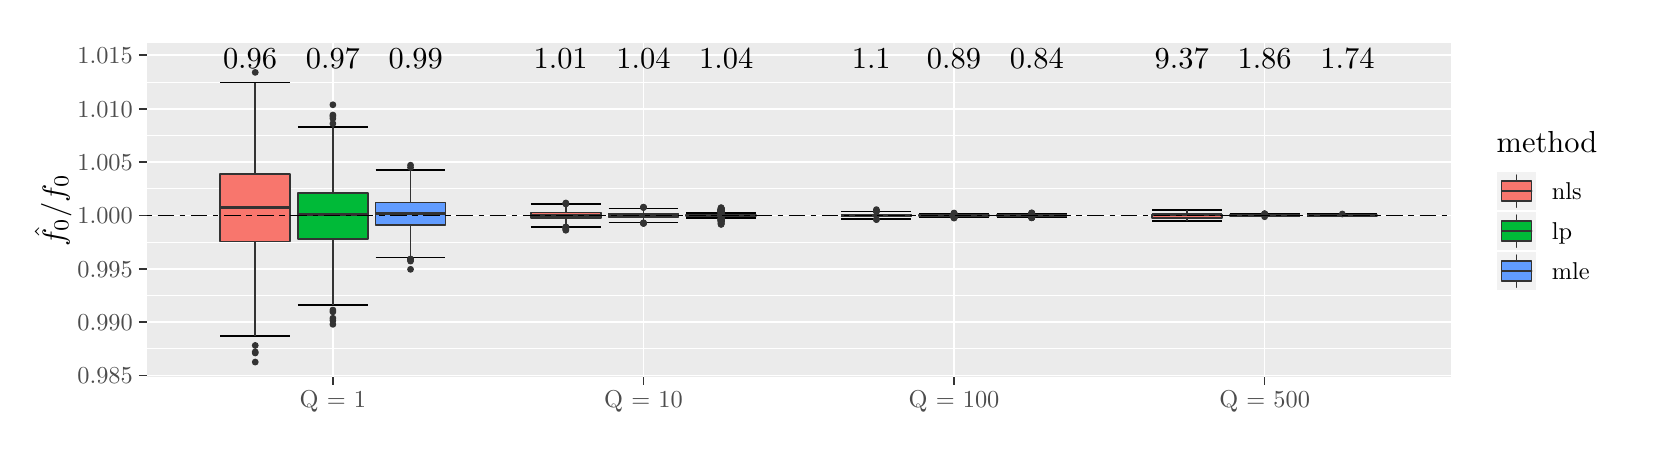
\begin{tikzpicture}[x=1pt,y=1pt]
\definecolor{fillColor}{RGB}{255,255,255}
\path[use as bounding box,fill=fillColor,fill opacity=0.00] (0,0) rectangle (578.16,144.54);
\begin{scope}
\path[clip] (  0.00,  0.00) rectangle (578.16,144.54);
\definecolor{drawColor}{RGB}{255,255,255}
\definecolor{fillColor}{RGB}{255,255,255}

\path[draw=drawColor,line width= 0.6pt,line join=round,line cap=round,fill=fillColor] (  0.00,  0.00) rectangle (578.16,144.54);
\end{scope}
\begin{scope}
\path[clip] ( 42.95, 18.22) rectangle (514.31,139.04);
\definecolor{fillColor}{gray}{0.92}

\path[fill=fillColor] ( 42.95, 18.22) rectangle (514.31,139.04);
\definecolor{drawColor}{RGB}{255,255,255}

\path[draw=drawColor,line width= 0.3pt,line join=round] ( 42.95, 28.49) --
	(514.31, 28.49);

\path[draw=drawColor,line width= 0.3pt,line join=round] ( 42.95, 47.77) --
	(514.31, 47.77);

\path[draw=drawColor,line width= 0.3pt,line join=round] ( 42.95, 67.06) --
	(514.31, 67.06);

\path[draw=drawColor,line width= 0.3pt,line join=round] ( 42.95, 86.34) --
	(514.31, 86.34);

\path[draw=drawColor,line width= 0.3pt,line join=round] ( 42.95,105.63) --
	(514.31,105.63);

\path[draw=drawColor,line width= 0.3pt,line join=round] ( 42.95,124.91) --
	(514.31,124.91);

\path[draw=drawColor,line width= 0.6pt,line join=round] ( 42.95, 18.84) --
	(514.31, 18.84);

\path[draw=drawColor,line width= 0.6pt,line join=round] ( 42.95, 38.13) --
	(514.31, 38.13);

\path[draw=drawColor,line width= 0.6pt,line join=round] ( 42.95, 57.41) --
	(514.31, 57.41);

\path[draw=drawColor,line width= 0.6pt,line join=round] ( 42.95, 76.70) --
	(514.31, 76.70);

\path[draw=drawColor,line width= 0.6pt,line join=round] ( 42.95, 95.99) --
	(514.31, 95.99);

\path[draw=drawColor,line width= 0.6pt,line join=round] ( 42.95,115.27) --
	(514.31,115.27);

\path[draw=drawColor,line width= 0.6pt,line join=round] ( 42.95,134.56) --
	(514.31,134.56);

\path[draw=drawColor,line width= 0.6pt,line join=round] (110.29, 18.22) --
	(110.29,139.04);

\path[draw=drawColor,line width= 0.6pt,line join=round] (222.52, 18.22) --
	(222.52,139.04);

\path[draw=drawColor,line width= 0.6pt,line join=round] (334.74, 18.22) --
	(334.74,139.04);

\path[draw=drawColor,line width= 0.6pt,line join=round] (446.97, 18.22) --
	(446.97,139.04);
\definecolor{drawColor}{RGB}{0,0,0}

\path[draw=drawColor,line width= 0.6pt,line join=round] ( 69.61,124.67) --
	( 94.86,124.67);

\path[draw=drawColor,line width= 0.6pt,line join=round] ( 82.23,124.67) --
	( 82.23, 33.03);

\path[draw=drawColor,line width= 0.6pt,line join=round] ( 69.61, 33.03) --
	( 94.86, 33.03);

\path[draw=drawColor,line width= 0.6pt,line join=round] ( 97.66,108.56) --
	(122.92,108.56);

\path[draw=drawColor,line width= 0.6pt,line join=round] (110.29,108.56) --
	(110.29, 44.37);

\path[draw=drawColor,line width= 0.6pt,line join=round] ( 97.66, 44.37) --
	(122.92, 44.37);

\path[draw=drawColor,line width= 0.6pt,line join=round] (125.72, 93.16) --
	(150.97, 93.16);

\path[draw=drawColor,line width= 0.6pt,line join=round] (138.35, 93.16) --
	(138.35, 61.46);

\path[draw=drawColor,line width= 0.6pt,line join=round] (125.72, 61.46) --
	(150.97, 61.46);

\path[draw=drawColor,line width= 0.6pt,line join=round] (181.83, 80.83) --
	(207.09, 80.83);

\path[draw=drawColor,line width= 0.6pt,line join=round] (194.46, 80.83) --
	(194.46, 72.57);

\path[draw=drawColor,line width= 0.6pt,line join=round] (181.83, 72.57) --
	(207.09, 72.57);

\path[draw=drawColor,line width= 0.6pt,line join=round] (209.89, 79.17) --
	(235.14, 79.17);

\path[draw=drawColor,line width= 0.6pt,line join=round] (222.52, 79.17) --
	(222.52, 74.08);

\path[draw=drawColor,line width= 0.6pt,line join=round] (209.89, 74.08) --
	(235.14, 74.08);

\path[draw=drawColor,line width= 0.6pt,line join=round] (237.95, 77.51) --
	(263.20, 77.51);

\path[draw=drawColor,line width= 0.6pt,line join=round] (250.57, 77.51) --
	(250.57, 75.79);

\path[draw=drawColor,line width= 0.6pt,line join=round] (237.95, 75.79) --
	(263.20, 75.79);

\path[draw=drawColor,line width= 0.6pt,line join=round] (294.06, 78.07) --
	(319.31, 78.07);

\path[draw=drawColor,line width= 0.6pt,line join=round] (306.69, 78.07) --
	(306.69, 75.32);

\path[draw=drawColor,line width= 0.6pt,line join=round] (294.06, 75.32) --
	(319.31, 75.32);

\path[draw=drawColor,line width= 0.6pt,line join=round] (322.12, 77.36) --
	(347.37, 77.36);

\path[draw=drawColor,line width= 0.6pt,line join=round] (334.74, 77.36) --
	(334.74, 76.00);

\path[draw=drawColor,line width= 0.6pt,line join=round] (322.12, 76.00) --
	(347.37, 76.00);

\path[draw=drawColor,line width= 0.6pt,line join=round] (350.18, 77.37) --
	(375.43, 77.37);

\path[draw=drawColor,line width= 0.6pt,line join=round] (362.80, 77.37) --
	(362.80, 76.00);

\path[draw=drawColor,line width= 0.6pt,line join=round] (350.18, 76.00) --
	(375.43, 76.00);

\path[draw=drawColor,line width= 0.6pt,line join=round] (406.29, 78.73) --
	(431.54, 78.73);

\path[draw=drawColor,line width= 0.6pt,line join=round] (418.91, 78.73) --
	(418.91, 74.74);

\path[draw=drawColor,line width= 0.6pt,line join=round] (406.29, 74.74) --
	(431.54, 74.74);

\path[draw=drawColor,line width= 0.6pt,line join=round] (434.35, 77.15) --
	(459.60, 77.15);

\path[draw=drawColor,line width= 0.6pt,line join=round] (446.97, 77.15) --
	(446.97, 76.26);

\path[draw=drawColor,line width= 0.6pt,line join=round] (434.35, 76.26) --
	(459.60, 76.26);

\path[draw=drawColor,line width= 0.6pt,line join=round] (462.40, 77.16) --
	(487.65, 77.16);

\path[draw=drawColor,line width= 0.6pt,line join=round] (475.03, 77.16) --
	(475.03, 76.27);

\path[draw=drawColor,line width= 0.6pt,line join=round] (462.40, 76.27) --
	(487.65, 76.27);
\definecolor{drawColor}{gray}{0.20}
\definecolor{fillColor}{gray}{0.20}

\path[draw=drawColor,line width= 0.4pt,line join=round,line cap=round,fill=fillColor] ( 82.23, 27.38) circle (  1.02);

\path[draw=drawColor,line width= 0.4pt,line join=round,line cap=round,fill=fillColor] ( 82.23, 23.71) circle (  1.02);

\path[draw=drawColor,line width= 0.4pt,line join=round,line cap=round,fill=fillColor] ( 82.23,128.38) circle (  1.02);

\path[draw=drawColor,line width= 0.4pt,line join=round,line cap=round,fill=fillColor] ( 82.23, 29.71) circle (  1.02);

\path[draw=drawColor,line width= 0.4pt,line join=round,line cap=round,fill=fillColor] ( 82.23, 26.99) circle (  1.02);

\path[draw=drawColor,line width= 0.6pt,line join=round] ( 82.23, 91.70) -- ( 82.23,124.67);

\path[draw=drawColor,line width= 0.6pt,line join=round] ( 82.23, 67.31) -- ( 82.23, 33.03);
\definecolor{fillColor}{RGB}{248,118,109}

\path[draw=drawColor,line width= 0.6pt,line join=round,line cap=round,fill=fillColor] ( 69.61, 91.70) --
	( 69.61, 67.31) --
	( 94.86, 67.31) --
	( 94.86, 91.70) --
	( 69.61, 91.70) --
	cycle;

\path[draw=drawColor,line width= 1.1pt,line join=round] ( 69.61, 79.60) -- ( 94.86, 79.60);
\definecolor{fillColor}{gray}{0.20}

\path[draw=drawColor,line width= 0.4pt,line join=round,line cap=round,fill=fillColor] (110.29,112.98) circle (  1.02);

\path[draw=drawColor,line width= 0.4pt,line join=round,line cap=round,fill=fillColor] (110.29, 38.76) circle (  1.02);

\path[draw=drawColor,line width= 0.4pt,line join=round,line cap=round,fill=fillColor] (110.29,112.53) circle (  1.02);

\path[draw=drawColor,line width= 0.4pt,line join=round,line cap=round,fill=fillColor] (110.29,109.87) circle (  1.02);

\path[draw=drawColor,line width= 0.4pt,line join=round,line cap=round,fill=fillColor] (110.29,116.68) circle (  1.02);

\path[draw=drawColor,line width= 0.4pt,line join=round,line cap=round,fill=fillColor] (110.29, 37.34) circle (  1.02);

\path[draw=drawColor,line width= 0.4pt,line join=round,line cap=round,fill=fillColor] (110.29, 42.51) circle (  1.02);

\path[draw=drawColor,line width= 0.4pt,line join=round,line cap=round,fill=fillColor] (110.29,111.73) circle (  1.02);

\path[draw=drawColor,line width= 0.4pt,line join=round,line cap=round,fill=fillColor] (110.29, 39.55) circle (  1.02);

\path[draw=drawColor,line width= 0.4pt,line join=round,line cap=round,fill=fillColor] (110.29, 41.85) circle (  1.02);

\path[draw=drawColor,line width= 0.6pt,line join=round] (110.29, 84.71) -- (110.29,108.56);

\path[draw=drawColor,line width= 0.6pt,line join=round] (110.29, 68.07) -- (110.29, 44.37);
\definecolor{fillColor}{RGB}{0,186,56}

\path[draw=drawColor,line width= 0.6pt,line join=round,line cap=round,fill=fillColor] ( 97.66, 84.71) --
	( 97.66, 68.07) --
	(122.92, 68.07) --
	(122.92, 84.71) --
	( 97.66, 84.71) --
	cycle;

\path[draw=drawColor,line width= 1.1pt,line join=round] ( 97.66, 77.11) -- (122.92, 77.11);
\definecolor{fillColor}{gray}{0.20}

\path[draw=drawColor,line width= 0.4pt,line join=round,line cap=round,fill=fillColor] (138.35, 60.83) circle (  1.02);

\path[draw=drawColor,line width= 0.4pt,line join=round,line cap=round,fill=fillColor] (138.35, 60.81) circle (  1.02);

\path[draw=drawColor,line width= 0.4pt,line join=round,line cap=round,fill=fillColor] (138.35, 57.21) circle (  1.02);

\path[draw=drawColor,line width= 0.4pt,line join=round,line cap=round,fill=fillColor] (138.35, 60.94) circle (  1.02);

\path[draw=drawColor,line width= 0.4pt,line join=round,line cap=round,fill=fillColor] (138.35, 93.99) circle (  1.02);

\path[draw=drawColor,line width= 0.4pt,line join=round,line cap=round,fill=fillColor] (138.35, 94.85) circle (  1.02);

\path[draw=drawColor,line width= 0.4pt,line join=round,line cap=round,fill=fillColor] (138.35, 60.19) circle (  1.02);

\path[draw=drawColor,line width= 0.6pt,line join=round] (138.35, 81.33) -- (138.35, 93.16);

\path[draw=drawColor,line width= 0.6pt,line join=round] (138.35, 73.35) -- (138.35, 61.46);
\definecolor{fillColor}{RGB}{97,156,255}

\path[draw=drawColor,line width= 0.6pt,line join=round,line cap=round,fill=fillColor] (125.72, 81.33) --
	(125.72, 73.35) --
	(150.97, 73.35) --
	(150.97, 81.33) --
	(125.72, 81.33) --
	cycle;

\path[draw=drawColor,line width= 1.1pt,line join=round] (125.72, 77.45) -- (150.97, 77.45);
\definecolor{fillColor}{gray}{0.20}

\path[draw=drawColor,line width= 0.4pt,line join=round,line cap=round,fill=fillColor] (194.46, 71.34) circle (  1.02);

\path[draw=drawColor,line width= 0.4pt,line join=round,line cap=round,fill=fillColor] (194.46, 72.39) circle (  1.02);

\path[draw=drawColor,line width= 0.4pt,line join=round,line cap=round,fill=fillColor] (194.46, 72.40) circle (  1.02);

\path[draw=drawColor,line width= 0.4pt,line join=round,line cap=round,fill=fillColor] (194.46, 71.56) circle (  1.02);

\path[draw=drawColor,line width= 0.4pt,line join=round,line cap=round,fill=fillColor] (194.46, 71.97) circle (  1.02);

\path[draw=drawColor,line width= 0.4pt,line join=round,line cap=round,fill=fillColor] (194.46, 72.45) circle (  1.02);

\path[draw=drawColor,line width= 0.4pt,line join=round,line cap=round,fill=fillColor] (194.46, 80.94) circle (  1.02);

\path[draw=drawColor,line width= 0.4pt,line join=round,line cap=round,fill=fillColor] (194.46, 81.19) circle (  1.02);

\path[draw=drawColor,line width= 0.4pt,line join=round,line cap=round,fill=fillColor] (194.46, 80.86) circle (  1.02);

\path[draw=drawColor,line width= 0.4pt,line join=round,line cap=round,fill=fillColor] (194.46, 72.52) circle (  1.02);

\path[draw=drawColor,line width= 0.4pt,line join=round,line cap=round,fill=fillColor] (194.46, 72.35) circle (  1.02);

\path[draw=drawColor,line width= 0.6pt,line join=round] (194.46, 77.73) -- (194.46, 80.83);

\path[draw=drawColor,line width= 0.6pt,line join=round] (194.46, 75.65) -- (194.46, 72.57);
\definecolor{fillColor}{RGB}{248,118,109}

\path[draw=drawColor,line width= 0.6pt,line join=round,line cap=round,fill=fillColor] (181.83, 77.73) --
	(181.83, 75.65) --
	(207.09, 75.65) --
	(207.09, 77.73) --
	(181.83, 77.73) --
	cycle;

\path[draw=drawColor,line width= 1.1pt,line join=round] (181.83, 76.53) -- (207.09, 76.53);
\definecolor{fillColor}{gray}{0.20}

\path[draw=drawColor,line width= 0.4pt,line join=round,line cap=round,fill=fillColor] (222.52, 73.80) circle (  1.02);

\path[draw=drawColor,line width= 0.4pt,line join=round,line cap=round,fill=fillColor] (222.52, 74.02) circle (  1.02);

\path[draw=drawColor,line width= 0.4pt,line join=round,line cap=round,fill=fillColor] (222.52, 79.57) circle (  1.02);

\path[draw=drawColor,line width= 0.4pt,line join=round,line cap=round,fill=fillColor] (222.52, 79.63) circle (  1.02);

\path[draw=drawColor,line width= 0.4pt,line join=round,line cap=round,fill=fillColor] (222.52, 73.91) circle (  1.02);

\path[draw=drawColor,line width= 0.4pt,line join=round,line cap=round,fill=fillColor] (222.52, 73.82) circle (  1.02);

\path[draw=drawColor,line width= 0.4pt,line join=round,line cap=round,fill=fillColor] (222.52, 79.63) circle (  1.02);

\path[draw=drawColor,line width= 0.6pt,line join=round] (222.52, 77.34) -- (222.52, 79.17);

\path[draw=drawColor,line width= 0.6pt,line join=round] (222.52, 76.02) -- (222.52, 74.08);
\definecolor{fillColor}{RGB}{0,186,56}

\path[draw=drawColor,line width= 0.6pt,line join=round,line cap=round,fill=fillColor] (209.89, 77.34) --
	(209.89, 76.02) --
	(235.14, 76.02) --
	(235.14, 77.34) --
	(209.89, 77.34) --
	cycle;

\path[draw=drawColor,line width= 1.1pt,line join=round] (209.89, 76.68) -- (235.14, 76.68);
\definecolor{fillColor}{gray}{0.20}

\path[draw=drawColor,line width= 0.4pt,line join=round,line cap=round,fill=fillColor] (250.57, 77.89) circle (  1.02);

\path[draw=drawColor,line width= 0.4pt,line join=round,line cap=round,fill=fillColor] (250.57, 75.45) circle (  1.02);

\path[draw=drawColor,line width= 0.4pt,line join=round,line cap=round,fill=fillColor] (250.57, 77.80) circle (  1.02);

\path[draw=drawColor,line width= 0.4pt,line join=round,line cap=round,fill=fillColor] (250.57, 78.38) circle (  1.02);

\path[draw=drawColor,line width= 0.4pt,line join=round,line cap=round,fill=fillColor] (250.57, 78.67) circle (  1.02);

\path[draw=drawColor,line width= 0.4pt,line join=round,line cap=round,fill=fillColor] (250.57, 77.74) circle (  1.02);

\path[draw=drawColor,line width= 0.4pt,line join=round,line cap=round,fill=fillColor] (250.57, 78.49) circle (  1.02);

\path[draw=drawColor,line width= 0.4pt,line join=round,line cap=round,fill=fillColor] (250.57, 75.35) circle (  1.02);

\path[draw=drawColor,line width= 0.4pt,line join=round,line cap=round,fill=fillColor] (250.57, 78.21) circle (  1.02);

\path[draw=drawColor,line width= 0.4pt,line join=round,line cap=round,fill=fillColor] (250.57, 77.53) circle (  1.02);

\path[draw=drawColor,line width= 0.4pt,line join=round,line cap=round,fill=fillColor] (250.57, 73.79) circle (  1.02);

\path[draw=drawColor,line width= 0.4pt,line join=round,line cap=round,fill=fillColor] (250.57, 78.25) circle (  1.02);

\path[draw=drawColor,line width= 0.4pt,line join=round,line cap=round,fill=fillColor] (250.57, 77.92) circle (  1.02);

\path[draw=drawColor,line width= 0.4pt,line join=round,line cap=round,fill=fillColor] (250.57, 78.99) circle (  1.02);

\path[draw=drawColor,line width= 0.4pt,line join=round,line cap=round,fill=fillColor] (250.57, 78.54) circle (  1.02);

\path[draw=drawColor,line width= 0.4pt,line join=round,line cap=round,fill=fillColor] (250.57, 73.90) circle (  1.02);

\path[draw=drawColor,line width= 0.4pt,line join=round,line cap=round,fill=fillColor] (250.57, 78.54) circle (  1.02);

\path[draw=drawColor,line width= 0.4pt,line join=round,line cap=round,fill=fillColor] (250.57, 78.31) circle (  1.02);

\path[draw=drawColor,line width= 0.4pt,line join=round,line cap=round,fill=fillColor] (250.57, 78.07) circle (  1.02);

\path[draw=drawColor,line width= 0.4pt,line join=round,line cap=round,fill=fillColor] (250.57, 78.13) circle (  1.02);

\path[draw=drawColor,line width= 0.4pt,line join=round,line cap=round,fill=fillColor] (250.57, 78.41) circle (  1.02);

\path[draw=drawColor,line width= 0.4pt,line join=round,line cap=round,fill=fillColor] (250.57, 75.69) circle (  1.02);

\path[draw=drawColor,line width= 0.4pt,line join=round,line cap=round,fill=fillColor] (250.57, 74.87) circle (  1.02);

\path[draw=drawColor,line width= 0.4pt,line join=round,line cap=round,fill=fillColor] (250.57, 78.71) circle (  1.02);

\path[draw=drawColor,line width= 0.4pt,line join=round,line cap=round,fill=fillColor] (250.57, 74.37) circle (  1.02);

\path[draw=drawColor,line width= 0.4pt,line join=round,line cap=round,fill=fillColor] (250.57, 77.56) circle (  1.02);

\path[draw=drawColor,line width= 0.4pt,line join=round,line cap=round,fill=fillColor] (250.57, 77.61) circle (  1.02);

\path[draw=drawColor,line width= 0.4pt,line join=round,line cap=round,fill=fillColor] (250.57, 78.44) circle (  1.02);

\path[draw=drawColor,line width= 0.4pt,line join=round,line cap=round,fill=fillColor] (250.57, 78.83) circle (  1.02);

\path[draw=drawColor,line width= 0.4pt,line join=round,line cap=round,fill=fillColor] (250.57, 75.38) circle (  1.02);

\path[draw=drawColor,line width= 0.4pt,line join=round,line cap=round,fill=fillColor] (250.57, 77.91) circle (  1.02);

\path[draw=drawColor,line width= 0.4pt,line join=round,line cap=round,fill=fillColor] (250.57, 78.06) circle (  1.02);

\path[draw=drawColor,line width= 0.4pt,line join=round,line cap=round,fill=fillColor] (250.57, 74.71) circle (  1.02);

\path[draw=drawColor,line width= 0.4pt,line join=round,line cap=round,fill=fillColor] (250.57, 78.86) circle (  1.02);

\path[draw=drawColor,line width= 0.4pt,line join=round,line cap=round,fill=fillColor] (250.57, 79.32) circle (  1.02);

\path[draw=drawColor,line width= 0.4pt,line join=round,line cap=round,fill=fillColor] (250.57, 79.41) circle (  1.02);

\path[draw=drawColor,line width= 0.4pt,line join=round,line cap=round,fill=fillColor] (250.57, 75.15) circle (  1.02);

\path[draw=drawColor,line width= 0.4pt,line join=round,line cap=round,fill=fillColor] (250.57, 77.84) circle (  1.02);

\path[draw=drawColor,line width= 0.4pt,line join=round,line cap=round,fill=fillColor] (250.57, 78.81) circle (  1.02);

\path[draw=drawColor,line width= 0.4pt,line join=round,line cap=round,fill=fillColor] (250.57, 75.69) circle (  1.02);

\path[draw=drawColor,line width= 0.4pt,line join=round,line cap=round,fill=fillColor] (250.57, 74.73) circle (  1.02);

\path[draw=drawColor,line width= 0.4pt,line join=round,line cap=round,fill=fillColor] (250.57, 77.56) circle (  1.02);

\path[draw=drawColor,line width= 0.4pt,line join=round,line cap=round,fill=fillColor] (250.57, 78.14) circle (  1.02);

\path[draw=drawColor,line width= 0.4pt,line join=round,line cap=round,fill=fillColor] (250.57, 79.19) circle (  1.02);

\path[draw=drawColor,line width= 0.4pt,line join=round,line cap=round,fill=fillColor] (250.57, 77.82) circle (  1.02);

\path[draw=drawColor,line width= 0.4pt,line join=round,line cap=round,fill=fillColor] (250.57, 74.92) circle (  1.02);

\path[draw=drawColor,line width= 0.4pt,line join=round,line cap=round,fill=fillColor] (250.57, 77.65) circle (  1.02);

\path[draw=drawColor,line width= 0.4pt,line join=round,line cap=round,fill=fillColor] (250.57, 75.70) circle (  1.02);

\path[draw=drawColor,line width= 0.4pt,line join=round,line cap=round,fill=fillColor] (250.57, 78.04) circle (  1.02);

\path[draw=drawColor,line width= 0.4pt,line join=round,line cap=round,fill=fillColor] (250.57, 77.94) circle (  1.02);

\path[draw=drawColor,line width= 0.4pt,line join=round,line cap=round,fill=fillColor] (250.57, 75.51) circle (  1.02);

\path[draw=drawColor,line width= 0.4pt,line join=round,line cap=round,fill=fillColor] (250.57, 78.28) circle (  1.02);

\path[draw=drawColor,line width= 0.4pt,line join=round,line cap=round,fill=fillColor] (250.57, 75.06) circle (  1.02);

\path[draw=drawColor,line width= 0.4pt,line join=round,line cap=round,fill=fillColor] (250.57, 77.72) circle (  1.02);

\path[draw=drawColor,line width= 0.4pt,line join=round,line cap=round,fill=fillColor] (250.57, 75.71) circle (  1.02);

\path[draw=drawColor,line width= 0.4pt,line join=round,line cap=round,fill=fillColor] (250.57, 77.88) circle (  1.02);

\path[draw=drawColor,line width= 0.4pt,line join=round,line cap=round,fill=fillColor] (250.57, 78.89) circle (  1.02);

\path[draw=drawColor,line width= 0.4pt,line join=round,line cap=round,fill=fillColor] (250.57, 78.56) circle (  1.02);

\path[draw=drawColor,line width= 0.4pt,line join=round,line cap=round,fill=fillColor] (250.57, 79.10) circle (  1.02);

\path[draw=drawColor,line width= 0.4pt,line join=round,line cap=round,fill=fillColor] (250.57, 74.80) circle (  1.02);

\path[draw=drawColor,line width= 0.4pt,line join=round,line cap=round,fill=fillColor] (250.57, 73.50) circle (  1.02);

\path[draw=drawColor,line width= 0.4pt,line join=round,line cap=round,fill=fillColor] (250.57, 78.17) circle (  1.02);

\path[draw=drawColor,line width= 0.4pt,line join=round,line cap=round,fill=fillColor] (250.57, 77.86) circle (  1.02);

\path[draw=drawColor,line width= 0.4pt,line join=round,line cap=round,fill=fillColor] (250.57, 78.34) circle (  1.02);

\path[draw=drawColor,line width= 0.4pt,line join=round,line cap=round,fill=fillColor] (250.57, 78.66) circle (  1.02);

\path[draw=drawColor,line width= 0.4pt,line join=round,line cap=round,fill=fillColor] (250.57, 78.01) circle (  1.02);

\path[draw=drawColor,line width= 0.4pt,line join=round,line cap=round,fill=fillColor] (250.57, 77.72) circle (  1.02);

\path[draw=drawColor,line width= 0.4pt,line join=round,line cap=round,fill=fillColor] (250.57, 78.07) circle (  1.02);

\path[draw=drawColor,line width= 0.4pt,line join=round,line cap=round,fill=fillColor] (250.57, 74.77) circle (  1.02);

\path[draw=drawColor,line width= 0.4pt,line join=round,line cap=round,fill=fillColor] (250.57, 74.04) circle (  1.02);

\path[draw=drawColor,line width= 0.4pt,line join=round,line cap=round,fill=fillColor] (250.57, 74.66) circle (  1.02);

\path[draw=drawColor,line width= 0.4pt,line join=round,line cap=round,fill=fillColor] (250.57, 78.26) circle (  1.02);

\path[draw=drawColor,line width= 0.4pt,line join=round,line cap=round,fill=fillColor] (250.57, 78.12) circle (  1.02);

\path[draw=drawColor,line width= 0.4pt,line join=round,line cap=round,fill=fillColor] (250.57, 77.67) circle (  1.02);

\path[draw=drawColor,line width= 0.4pt,line join=round,line cap=round,fill=fillColor] (250.57, 78.84) circle (  1.02);

\path[draw=drawColor,line width= 0.4pt,line join=round,line cap=round,fill=fillColor] (250.57, 74.88) circle (  1.02);

\path[draw=drawColor,line width= 0.4pt,line join=round,line cap=round,fill=fillColor] (250.57, 78.62) circle (  1.02);

\path[draw=drawColor,line width= 0.4pt,line join=round,line cap=round,fill=fillColor] (250.57, 77.86) circle (  1.02);

\path[draw=drawColor,line width= 0.4pt,line join=round,line cap=round,fill=fillColor] (250.57, 77.62) circle (  1.02);

\path[draw=drawColor,line width= 0.4pt,line join=round,line cap=round,fill=fillColor] (250.57, 78.13) circle (  1.02);

\path[draw=drawColor,line width= 0.4pt,line join=round,line cap=round,fill=fillColor] (250.57, 78.33) circle (  1.02);

\path[draw=drawColor,line width= 0.4pt,line join=round,line cap=round,fill=fillColor] (250.57, 77.85) circle (  1.02);

\path[draw=drawColor,line width= 0.4pt,line join=round,line cap=round,fill=fillColor] (250.57, 75.58) circle (  1.02);

\path[draw=drawColor,line width= 0.4pt,line join=round,line cap=round,fill=fillColor] (250.57, 77.78) circle (  1.02);

\path[draw=drawColor,line width= 0.4pt,line join=round,line cap=round,fill=fillColor] (250.57, 75.34) circle (  1.02);

\path[draw=drawColor,line width= 0.4pt,line join=round,line cap=round,fill=fillColor] (250.57, 77.56) circle (  1.02);

\path[draw=drawColor,line width= 0.4pt,line join=round,line cap=round,fill=fillColor] (250.57, 78.40) circle (  1.02);

\path[draw=drawColor,line width= 0.4pt,line join=round,line cap=round,fill=fillColor] (250.57, 75.21) circle (  1.02);

\path[draw=drawColor,line width= 0.4pt,line join=round,line cap=round,fill=fillColor] (250.57, 74.39) circle (  1.02);

\path[draw=drawColor,line width= 0.4pt,line join=round,line cap=round,fill=fillColor] (250.57, 77.71) circle (  1.02);

\path[draw=drawColor,line width= 0.4pt,line join=round,line cap=round,fill=fillColor] (250.57, 78.10) circle (  1.02);

\path[draw=drawColor,line width= 0.4pt,line join=round,line cap=round,fill=fillColor] (250.57, 78.20) circle (  1.02);

\path[draw=drawColor,line width= 0.4pt,line join=round,line cap=round,fill=fillColor] (250.57, 78.03) circle (  1.02);

\path[draw=drawColor,line width= 0.4pt,line join=round,line cap=round,fill=fillColor] (250.57, 74.50) circle (  1.02);

\path[draw=drawColor,line width= 0.4pt,line join=round,line cap=round,fill=fillColor] (250.57, 78.71) circle (  1.02);

\path[draw=drawColor,line width= 0.4pt,line join=round,line cap=round,fill=fillColor] (250.57, 77.69) circle (  1.02);

\path[draw=drawColor,line width= 0.4pt,line join=round,line cap=round,fill=fillColor] (250.57, 79.12) circle (  1.02);

\path[draw=drawColor,line width= 0.4pt,line join=round,line cap=round,fill=fillColor] (250.57, 78.73) circle (  1.02);

\path[draw=drawColor,line width= 0.4pt,line join=round,line cap=round,fill=fillColor] (250.57, 75.30) circle (  1.02);

\path[draw=drawColor,line width= 0.4pt,line join=round,line cap=round,fill=fillColor] (250.57, 77.66) circle (  1.02);

\path[draw=drawColor,line width= 0.4pt,line join=round,line cap=round,fill=fillColor] (250.57, 77.94) circle (  1.02);

\path[draw=drawColor,line width= 0.4pt,line join=round,line cap=round,fill=fillColor] (250.57, 78.60) circle (  1.02);

\path[draw=drawColor,line width= 0.4pt,line join=round,line cap=round,fill=fillColor] (250.57, 78.42) circle (  1.02);

\path[draw=drawColor,line width= 0.4pt,line join=round,line cap=round,fill=fillColor] (250.57, 77.56) circle (  1.02);

\path[draw=drawColor,line width= 0.4pt,line join=round,line cap=round,fill=fillColor] (250.57, 75.31) circle (  1.02);

\path[draw=drawColor,line width= 0.4pt,line join=round,line cap=round,fill=fillColor] (250.57, 78.62) circle (  1.02);

\path[draw=drawColor,line width= 0.4pt,line join=round,line cap=round,fill=fillColor] (250.57, 78.25) circle (  1.02);

\path[draw=drawColor,line width= 0.4pt,line join=round,line cap=round,fill=fillColor] (250.57, 75.66) circle (  1.02);

\path[draw=drawColor,line width= 0.4pt,line join=round,line cap=round,fill=fillColor] (250.57, 77.58) circle (  1.02);

\path[draw=drawColor,line width= 0.4pt,line join=round,line cap=round,fill=fillColor] (250.57, 77.70) circle (  1.02);

\path[draw=drawColor,line width= 0.4pt,line join=round,line cap=round,fill=fillColor] (250.57, 77.69) circle (  1.02);

\path[draw=drawColor,line width= 0.4pt,line join=round,line cap=round,fill=fillColor] (250.57, 78.44) circle (  1.02);

\path[draw=drawColor,line width= 0.4pt,line join=round,line cap=round,fill=fillColor] (250.57, 75.11) circle (  1.02);

\path[draw=drawColor,line width= 0.4pt,line join=round,line cap=round,fill=fillColor] (250.57, 73.63) circle (  1.02);

\path[draw=drawColor,line width= 0.4pt,line join=round,line cap=round,fill=fillColor] (250.57, 77.65) circle (  1.02);

\path[draw=drawColor,line width= 0.4pt,line join=round,line cap=round,fill=fillColor] (250.57, 78.52) circle (  1.02);

\path[draw=drawColor,line width= 0.4pt,line join=round,line cap=round,fill=fillColor] (250.57, 77.64) circle (  1.02);

\path[draw=drawColor,line width= 0.4pt,line join=round,line cap=round,fill=fillColor] (250.57, 77.77) circle (  1.02);

\path[draw=drawColor,line width= 0.4pt,line join=round,line cap=round,fill=fillColor] (250.57, 78.25) circle (  1.02);

\path[draw=drawColor,line width= 0.4pt,line join=round,line cap=round,fill=fillColor] (250.57, 77.88) circle (  1.02);

\path[draw=drawColor,line width= 0.4pt,line join=round,line cap=round,fill=fillColor] (250.57, 78.21) circle (  1.02);

\path[draw=drawColor,line width= 0.4pt,line join=round,line cap=round,fill=fillColor] (250.57, 77.68) circle (  1.02);

\path[draw=drawColor,line width= 0.4pt,line join=round,line cap=round,fill=fillColor] (250.57, 77.52) circle (  1.02);

\path[draw=drawColor,line width= 0.4pt,line join=round,line cap=round,fill=fillColor] (250.57, 78.49) circle (  1.02);

\path[draw=drawColor,line width= 0.4pt,line join=round,line cap=round,fill=fillColor] (250.57, 75.66) circle (  1.02);

\path[draw=drawColor,line width= 0.4pt,line join=round,line cap=round,fill=fillColor] (250.57, 75.54) circle (  1.02);

\path[draw=drawColor,line width= 0.4pt,line join=round,line cap=round,fill=fillColor] (250.57, 78.62) circle (  1.02);

\path[draw=drawColor,line width= 0.4pt,line join=round,line cap=round,fill=fillColor] (250.57, 78.07) circle (  1.02);

\path[draw=drawColor,line width= 0.4pt,line join=round,line cap=round,fill=fillColor] (250.57, 77.77) circle (  1.02);

\path[draw=drawColor,line width= 0.4pt,line join=round,line cap=round,fill=fillColor] (250.57, 73.49) circle (  1.02);

\path[draw=drawColor,line width= 0.4pt,line join=round,line cap=round,fill=fillColor] (250.57, 78.43) circle (  1.02);

\path[draw=drawColor,line width= 0.4pt,line join=round,line cap=round,fill=fillColor] (250.57, 78.13) circle (  1.02);

\path[draw=drawColor,line width= 0.4pt,line join=round,line cap=round,fill=fillColor] (250.57, 77.92) circle (  1.02);

\path[draw=drawColor,line width= 0.4pt,line join=round,line cap=round,fill=fillColor] (250.57, 75.76) circle (  1.02);

\path[draw=drawColor,line width= 0.4pt,line join=round,line cap=round,fill=fillColor] (250.57, 78.61) circle (  1.02);

\path[draw=drawColor,line width= 0.4pt,line join=round,line cap=round,fill=fillColor] (250.57, 77.63) circle (  1.02);

\path[draw=drawColor,line width= 0.4pt,line join=round,line cap=round,fill=fillColor] (250.57, 77.67) circle (  1.02);

\path[draw=drawColor,line width= 0.4pt,line join=round,line cap=round,fill=fillColor] (250.57, 75.03) circle (  1.02);

\path[draw=drawColor,line width= 0.4pt,line join=round,line cap=round,fill=fillColor] (250.57, 78.29) circle (  1.02);

\path[draw=drawColor,line width= 0.4pt,line join=round,line cap=round,fill=fillColor] (250.57, 75.76) circle (  1.02);

\path[draw=drawColor,line width= 0.4pt,line join=round,line cap=round,fill=fillColor] (250.57, 77.62) circle (  1.02);

\path[draw=drawColor,line width= 0.4pt,line join=round,line cap=round,fill=fillColor] (250.57, 78.20) circle (  1.02);

\path[draw=drawColor,line width= 0.4pt,line join=round,line cap=round,fill=fillColor] (250.57, 77.95) circle (  1.02);

\path[draw=drawColor,line width= 0.4pt,line join=round,line cap=round,fill=fillColor] (250.57, 77.96) circle (  1.02);

\path[draw=drawColor,line width= 0.4pt,line join=round,line cap=round,fill=fillColor] (250.57, 75.20) circle (  1.02);

\path[draw=drawColor,line width= 0.4pt,line join=round,line cap=round,fill=fillColor] (250.57, 75.51) circle (  1.02);

\path[draw=drawColor,line width= 0.4pt,line join=round,line cap=round,fill=fillColor] (250.57, 79.24) circle (  1.02);

\path[draw=drawColor,line width= 0.4pt,line join=round,line cap=round,fill=fillColor] (250.57, 77.69) circle (  1.02);

\path[draw=drawColor,line width= 0.4pt,line join=round,line cap=round,fill=fillColor] (250.57, 78.63) circle (  1.02);

\path[draw=drawColor,line width= 0.4pt,line join=round,line cap=round,fill=fillColor] (250.57, 77.60) circle (  1.02);

\path[draw=drawColor,line width= 0.4pt,line join=round,line cap=round,fill=fillColor] (250.57, 74.92) circle (  1.02);

\path[draw=drawColor,line width= 0.4pt,line join=round,line cap=round,fill=fillColor] (250.57, 77.78) circle (  1.02);

\path[draw=drawColor,line width= 0.4pt,line join=round,line cap=round,fill=fillColor] (250.57, 77.59) circle (  1.02);

\path[draw=drawColor,line width= 0.4pt,line join=round,line cap=round,fill=fillColor] (250.57, 75.73) circle (  1.02);

\path[draw=drawColor,line width= 0.4pt,line join=round,line cap=round,fill=fillColor] (250.57, 77.92) circle (  1.02);

\path[draw=drawColor,line width= 0.4pt,line join=round,line cap=round,fill=fillColor] (250.57, 79.49) circle (  1.02);

\path[draw=drawColor,line width= 0.6pt,line join=round] (250.57, 76.86) -- (250.57, 77.51);

\path[draw=drawColor,line width= 0.6pt,line join=round] (250.57, 76.42) -- (250.57, 75.79);
\definecolor{fillColor}{RGB}{97,156,255}

\path[draw=drawColor,line width= 0.6pt,line join=round,line cap=round,fill=fillColor] (237.95, 76.86) --
	(237.95, 76.42) --
	(263.20, 76.42) --
	(263.20, 76.86) --
	(237.95, 76.86) --
	cycle;

\path[draw=drawColor,line width= 1.1pt,line join=round] (237.95, 76.61) -- (263.20, 76.61);
\definecolor{fillColor}{gray}{0.20}

\path[draw=drawColor,line width= 0.4pt,line join=round,line cap=round,fill=fillColor] (306.69, 78.80) circle (  1.02);

\path[draw=drawColor,line width= 0.4pt,line join=round,line cap=round,fill=fillColor] (306.69, 75.28) circle (  1.02);

\path[draw=drawColor,line width= 0.4pt,line join=round,line cap=round,fill=fillColor] (306.69, 78.35) circle (  1.02);

\path[draw=drawColor,line width= 0.4pt,line join=round,line cap=round,fill=fillColor] (306.69, 78.15) circle (  1.02);

\path[draw=drawColor,line width= 0.4pt,line join=round,line cap=round,fill=fillColor] (306.69, 75.18) circle (  1.02);

\path[draw=drawColor,line width= 0.4pt,line join=round,line cap=round,fill=fillColor] (306.69, 78.13) circle (  1.02);

\path[draw=drawColor,line width= 0.6pt,line join=round] (306.69, 77.06) -- (306.69, 78.07);

\path[draw=drawColor,line width= 0.6pt,line join=round] (306.69, 76.36) -- (306.69, 75.32);
\definecolor{fillColor}{RGB}{248,118,109}

\path[draw=drawColor,line width= 0.6pt,line join=round,line cap=round,fill=fillColor] (294.06, 77.06) --
	(294.06, 76.36) --
	(319.31, 76.36) --
	(319.31, 77.06) --
	(294.06, 77.06) --
	cycle;

\path[draw=drawColor,line width= 1.1pt,line join=round] (294.06, 76.72) -- (319.31, 76.72);
\definecolor{fillColor}{gray}{0.20}

\path[draw=drawColor,line width= 0.4pt,line join=round,line cap=round,fill=fillColor] (334.74, 75.94) circle (  1.02);

\path[draw=drawColor,line width= 0.4pt,line join=round,line cap=round,fill=fillColor] (334.74, 75.77) circle (  1.02);

\path[draw=drawColor,line width= 0.4pt,line join=round,line cap=round,fill=fillColor] (334.74, 75.97) circle (  1.02);

\path[draw=drawColor,line width= 0.4pt,line join=round,line cap=round,fill=fillColor] (334.74, 75.94) circle (  1.02);

\path[draw=drawColor,line width= 0.4pt,line join=round,line cap=round,fill=fillColor] (334.74, 75.94) circle (  1.02);

\path[draw=drawColor,line width= 0.4pt,line join=round,line cap=round,fill=fillColor] (334.74, 77.41) circle (  1.02);

\path[draw=drawColor,line width= 0.4pt,line join=round,line cap=round,fill=fillColor] (334.74, 75.83) circle (  1.02);

\path[draw=drawColor,line width= 0.4pt,line join=round,line cap=round,fill=fillColor] (334.74, 77.55) circle (  1.02);

\path[draw=drawColor,line width= 0.4pt,line join=round,line cap=round,fill=fillColor] (334.74, 75.88) circle (  1.02);

\path[draw=drawColor,line width= 0.4pt,line join=round,line cap=round,fill=fillColor] (334.74, 77.41) circle (  1.02);

\path[draw=drawColor,line width= 0.4pt,line join=round,line cap=round,fill=fillColor] (334.74, 77.40) circle (  1.02);

\path[draw=drawColor,line width= 0.6pt,line join=round] (334.74, 76.86) -- (334.74, 77.36);

\path[draw=drawColor,line width= 0.6pt,line join=round] (334.74, 76.51) -- (334.74, 76.00);
\definecolor{fillColor}{RGB}{0,186,56}

\path[draw=drawColor,line width= 0.6pt,line join=round,line cap=round,fill=fillColor] (322.12, 76.86) --
	(322.12, 76.51) --
	(347.37, 76.51) --
	(347.37, 76.86) --
	(322.12, 76.86) --
	cycle;

\path[draw=drawColor,line width= 1.1pt,line join=round] (322.12, 76.68) -- (347.37, 76.68);
\definecolor{fillColor}{gray}{0.20}

\path[draw=drawColor,line width= 0.4pt,line join=round,line cap=round,fill=fillColor] (362.80, 75.85) circle (  1.02);

\path[draw=drawColor,line width= 0.4pt,line join=round,line cap=round,fill=fillColor] (362.80, 75.85) circle (  1.02);

\path[draw=drawColor,line width= 0.4pt,line join=round,line cap=round,fill=fillColor] (362.80, 75.96) circle (  1.02);

\path[draw=drawColor,line width= 0.4pt,line join=round,line cap=round,fill=fillColor] (362.80, 75.94) circle (  1.02);

\path[draw=drawColor,line width= 0.4pt,line join=round,line cap=round,fill=fillColor] (362.80, 77.47) circle (  1.02);

\path[draw=drawColor,line width= 0.4pt,line join=round,line cap=round,fill=fillColor] (362.80, 77.41) circle (  1.02);

\path[draw=drawColor,line width= 0.4pt,line join=round,line cap=round,fill=fillColor] (362.80, 75.86) circle (  1.02);

\path[draw=drawColor,line width= 0.4pt,line join=round,line cap=round,fill=fillColor] (362.80, 75.96) circle (  1.02);

\path[draw=drawColor,line width= 0.4pt,line join=round,line cap=round,fill=fillColor] (362.80, 77.41) circle (  1.02);

\path[draw=drawColor,line width= 0.4pt,line join=round,line cap=round,fill=fillColor] (362.80, 77.63) circle (  1.02);

\path[draw=drawColor,line width= 0.4pt,line join=round,line cap=round,fill=fillColor] (362.80, 75.98) circle (  1.02);

\path[draw=drawColor,line width= 0.4pt,line join=round,line cap=round,fill=fillColor] (362.80, 77.55) circle (  1.02);

\path[draw=drawColor,line width= 0.6pt,line join=round] (362.80, 76.86) -- (362.80, 77.37);

\path[draw=drawColor,line width= 0.6pt,line join=round] (362.80, 76.51) -- (362.80, 76.00);
\definecolor{fillColor}{RGB}{97,156,255}

\path[draw=drawColor,line width= 0.6pt,line join=round,line cap=round,fill=fillColor] (350.18, 76.86) --
	(350.18, 76.51) --
	(375.43, 76.51) --
	(375.43, 76.86) --
	(350.18, 76.86) --
	cycle;

\path[draw=drawColor,line width= 1.1pt,line join=round] (350.18, 76.69) -- (375.43, 76.69);

\path[draw=drawColor,line width= 0.6pt,line join=round] (418.91, 77.06) -- (418.91, 78.73);

\path[draw=drawColor,line width= 0.6pt,line join=round] (418.91, 75.87) -- (418.91, 74.74);
\definecolor{fillColor}{RGB}{248,118,109}

\path[draw=drawColor,line width= 0.6pt,line join=round,line cap=round,fill=fillColor] (406.29, 77.06) --
	(406.29, 75.87) --
	(431.54, 75.87) --
	(431.54, 77.06) --
	(406.29, 77.06) --
	cycle;

\path[draw=drawColor,line width= 1.1pt,line join=round] (406.29, 76.93) -- (431.54, 76.93);
\definecolor{fillColor}{gray}{0.20}

\path[draw=drawColor,line width= 0.4pt,line join=round,line cap=round,fill=fillColor] (446.97, 76.23) circle (  1.02);

\path[draw=drawColor,line width= 0.4pt,line join=round,line cap=round,fill=fillColor] (446.97, 77.18) circle (  1.02);

\path[draw=drawColor,line width= 0.4pt,line join=round,line cap=round,fill=fillColor] (446.97, 77.29) circle (  1.02);

\path[draw=drawColor,line width= 0.4pt,line join=round,line cap=round,fill=fillColor] (446.97, 77.18) circle (  1.02);

\path[draw=drawColor,line width= 0.4pt,line join=round,line cap=round,fill=fillColor] (446.97, 77.19) circle (  1.02);

\path[draw=drawColor,line width= 0.4pt,line join=round,line cap=round,fill=fillColor] (446.97, 77.28) circle (  1.02);

\path[draw=drawColor,line width= 0.6pt,line join=round] (446.97, 76.82) -- (446.97, 77.15);

\path[draw=drawColor,line width= 0.6pt,line join=round] (446.97, 76.60) -- (446.97, 76.26);
\definecolor{fillColor}{RGB}{0,186,56}

\path[draw=drawColor,line width= 0.6pt,line join=round,line cap=round,fill=fillColor] (434.35, 76.82) --
	(434.35, 76.60) --
	(459.60, 76.60) --
	(459.60, 76.82) --
	(434.35, 76.82) --
	cycle;

\path[draw=drawColor,line width= 1.1pt,line join=round] (434.35, 76.72) -- (459.60, 76.72);
\definecolor{fillColor}{gray}{0.20}

\path[draw=drawColor,line width= 0.4pt,line join=round,line cap=round,fill=fillColor] (475.03, 77.21) circle (  1.02);

\path[draw=drawColor,line width= 0.6pt,line join=round] (475.03, 76.83) -- (475.03, 77.16);

\path[draw=drawColor,line width= 0.6pt,line join=round] (475.03, 76.60) -- (475.03, 76.27);
\definecolor{fillColor}{RGB}{97,156,255}

\path[draw=drawColor,line width= 0.6pt,line join=round,line cap=round,fill=fillColor] (462.40, 76.83) --
	(462.40, 76.60) --
	(487.65, 76.60) --
	(487.65, 76.83) --
	(462.40, 76.83) --
	cycle;

\path[draw=drawColor,line width= 1.1pt,line join=round] (462.40, 76.71) -- (487.65, 76.71);
\definecolor{drawColor}{RGB}{0,0,0}

\path[draw=drawColor,line width= 0.6pt,dash pattern=on 2pt off 2pt on 6pt off 2pt ,line join=round] ( 42.95, 76.70) -- (514.31, 76.70);

\node[text=drawColor,anchor=base,inner sep=0pt, outer sep=0pt, scale=  1.10] at (140.22,129.75) {0.99};

\node[text=drawColor,anchor=base,inner sep=0pt, outer sep=0pt, scale=  1.10] at (110.29,129.75) {0.97};

\node[text=drawColor,anchor=base,inner sep=0pt, outer sep=0pt, scale=  1.10] at ( 80.36,129.75) {0.96};

\node[text=drawColor,anchor=base,inner sep=0pt, outer sep=0pt, scale=  1.10] at (252.44,129.75) {1.04};

\node[text=drawColor,anchor=base,inner sep=0pt, outer sep=0pt, scale=  1.10] at (222.52,129.75) {1.04};

\node[text=drawColor,anchor=base,inner sep=0pt, outer sep=0pt, scale=  1.10] at (192.59,129.75) {1.01};

\node[text=drawColor,anchor=base,inner sep=0pt, outer sep=0pt, scale=  1.10] at (364.67,129.75) {0.84};

\node[text=drawColor,anchor=base,inner sep=0pt, outer sep=0pt, scale=  1.10] at (334.74,129.75) {0.89};

\node[text=drawColor,anchor=base,inner sep=0pt, outer sep=0pt, scale=  1.10] at (304.82,129.75) {1.1};

\node[text=drawColor,anchor=base,inner sep=0pt, outer sep=0pt, scale=  1.10] at (476.90,129.75) {1.74};

\node[text=drawColor,anchor=base,inner sep=0pt, outer sep=0pt, scale=  1.10] at (446.97,129.75) {1.86};

\node[text=drawColor,anchor=base,inner sep=0pt, outer sep=0pt, scale=  1.10] at (417.04,129.75) {9.37};
\end{scope}
\begin{scope}
\path[clip] (  0.00,  0.00) rectangle (578.16,144.54);
\definecolor{drawColor}{gray}{0.30}

\node[text=drawColor,anchor=base east,inner sep=0pt, outer sep=0pt, scale=  0.88] at ( 38.00, 15.81) {0.985};

\node[text=drawColor,anchor=base east,inner sep=0pt, outer sep=0pt, scale=  0.88] at ( 38.00, 35.10) {0.990};

\node[text=drawColor,anchor=base east,inner sep=0pt, outer sep=0pt, scale=  0.88] at ( 38.00, 54.38) {0.995};

\node[text=drawColor,anchor=base east,inner sep=0pt, outer sep=0pt, scale=  0.88] at ( 38.00, 73.67) {1.000};

\node[text=drawColor,anchor=base east,inner sep=0pt, outer sep=0pt, scale=  0.88] at ( 38.00, 92.95) {1.005};

\node[text=drawColor,anchor=base east,inner sep=0pt, outer sep=0pt, scale=  0.88] at ( 38.00,112.24) {1.010};

\node[text=drawColor,anchor=base east,inner sep=0pt, outer sep=0pt, scale=  0.88] at ( 38.00,131.53) {1.015};
\end{scope}
\begin{scope}
\path[clip] (  0.00,  0.00) rectangle (578.16,144.54);
\definecolor{drawColor}{gray}{0.20}

\path[draw=drawColor,line width= 0.6pt,line join=round] ( 40.20, 18.84) --
	( 42.95, 18.84);

\path[draw=drawColor,line width= 0.6pt,line join=round] ( 40.20, 38.13) --
	( 42.95, 38.13);

\path[draw=drawColor,line width= 0.6pt,line join=round] ( 40.20, 57.41) --
	( 42.95, 57.41);

\path[draw=drawColor,line width= 0.6pt,line join=round] ( 40.20, 76.70) --
	( 42.95, 76.70);

\path[draw=drawColor,line width= 0.6pt,line join=round] ( 40.20, 95.99) --
	( 42.95, 95.99);

\path[draw=drawColor,line width= 0.6pt,line join=round] ( 40.20,115.27) --
	( 42.95,115.27);

\path[draw=drawColor,line width= 0.6pt,line join=round] ( 40.20,134.56) --
	( 42.95,134.56);
\end{scope}
\begin{scope}
\path[clip] (  0.00,  0.00) rectangle (578.16,144.54);
\definecolor{drawColor}{gray}{0.20}

\path[draw=drawColor,line width= 0.6pt,line join=round] (110.29, 15.47) --
	(110.29, 18.22);

\path[draw=drawColor,line width= 0.6pt,line join=round] (222.52, 15.47) --
	(222.52, 18.22);

\path[draw=drawColor,line width= 0.6pt,line join=round] (334.74, 15.47) --
	(334.74, 18.22);

\path[draw=drawColor,line width= 0.6pt,line join=round] (446.97, 15.47) --
	(446.97, 18.22);
\end{scope}
\begin{scope}
\path[clip] (  0.00,  0.00) rectangle (578.16,144.54);
\definecolor{drawColor}{gray}{0.30}

\node[text=drawColor,anchor=base,inner sep=0pt, outer sep=0pt, scale=  0.88] at (110.29,  7.21) {Q = 1};

\node[text=drawColor,anchor=base,inner sep=0pt, outer sep=0pt, scale=  0.88] at (222.52,  7.21) {Q = 10};

\node[text=drawColor,anchor=base,inner sep=0pt, outer sep=0pt, scale=  0.88] at (334.74,  7.21) {Q = 100};

\node[text=drawColor,anchor=base,inner sep=0pt, outer sep=0pt, scale=  0.88] at (446.97,  7.21) {Q = 500};
\end{scope}
\begin{scope}
\path[clip] (  0.00,  0.00) rectangle (578.16,144.54);
\definecolor{drawColor}{RGB}{0,0,0}

\node[text=drawColor,rotate= 90.00,anchor=base,inner sep=0pt, outer sep=0pt, scale=  1.10] at ( 13.08, 78.63) {$\hat{f_0}/f_0$};
\end{scope}
\begin{scope}
\path[clip] (  0.00,  0.00) rectangle (578.16,144.54);
\definecolor{fillColor}{RGB}{255,255,255}

\path[fill=fillColor] (525.31, 43.84) rectangle (572.66,113.42);
\end{scope}
\begin{scope}
\path[clip] (  0.00,  0.00) rectangle (578.16,144.54);
\definecolor{drawColor}{RGB}{0,0,0}

\node[text=drawColor,anchor=base west,inner sep=0pt, outer sep=0pt, scale=  1.10] at (530.81, 99.27) {method};
\end{scope}
\begin{scope}
\path[clip] (  0.00,  0.00) rectangle (578.16,144.54);
\definecolor{drawColor}{RGB}{255,255,255}
\definecolor{fillColor}{gray}{0.95}

\path[draw=drawColor,line width= 0.6pt,line join=round,line cap=round,fill=fillColor] (530.81, 78.25) rectangle (545.26, 92.70);
\end{scope}
\begin{scope}
\path[clip] (  0.00,  0.00) rectangle (578.16,144.54);
\definecolor{drawColor}{gray}{0.20}

\path[draw=drawColor,line width= 0.6pt,line join=round,line cap=round] (538.03, 79.70) --
	(538.03, 81.86);

\path[draw=drawColor,line width= 0.6pt,line join=round,line cap=round] (538.03, 89.09) --
	(538.03, 91.26);
\definecolor{fillColor}{RGB}{248,118,109}

\path[draw=drawColor,line width= 0.6pt,line join=round,line cap=round,fill=fillColor] (532.61, 81.86) rectangle (543.45, 89.09);

\path[draw=drawColor,line width= 0.6pt,line join=round,line cap=round] (532.61, 85.48) --
	(543.45, 85.48);
\end{scope}
\begin{scope}
\path[clip] (  0.00,  0.00) rectangle (578.16,144.54);
\definecolor{drawColor}{RGB}{255,255,255}
\definecolor{fillColor}{gray}{0.95}

\path[draw=drawColor,line width= 0.6pt,line join=round,line cap=round,fill=fillColor] (530.81, 63.80) rectangle (545.26, 78.25);
\end{scope}
\begin{scope}
\path[clip] (  0.00,  0.00) rectangle (578.16,144.54);
\definecolor{drawColor}{gray}{0.20}

\path[draw=drawColor,line width= 0.6pt,line join=round,line cap=round] (538.03, 65.24) --
	(538.03, 67.41);

\path[draw=drawColor,line width= 0.6pt,line join=round,line cap=round] (538.03, 74.64) --
	(538.03, 76.81);
\definecolor{fillColor}{RGB}{0,186,56}

\path[draw=drawColor,line width= 0.6pt,line join=round,line cap=round,fill=fillColor] (532.61, 67.41) rectangle (543.45, 74.64);

\path[draw=drawColor,line width= 0.6pt,line join=round,line cap=round] (532.61, 71.02) --
	(543.45, 71.02);
\end{scope}
\begin{scope}
\path[clip] (  0.00,  0.00) rectangle (578.16,144.54);
\definecolor{drawColor}{RGB}{255,255,255}
\definecolor{fillColor}{gray}{0.95}

\path[draw=drawColor,line width= 0.6pt,line join=round,line cap=round,fill=fillColor] (530.81, 49.34) rectangle (545.26, 63.80);
\end{scope}
\begin{scope}
\path[clip] (  0.00,  0.00) rectangle (578.16,144.54);
\definecolor{drawColor}{gray}{0.20}

\path[draw=drawColor,line width= 0.6pt,line join=round,line cap=round] (538.03, 50.79) --
	(538.03, 52.96);

\path[draw=drawColor,line width= 0.6pt,line join=round,line cap=round] (538.03, 60.18) --
	(538.03, 62.35);
\definecolor{fillColor}{RGB}{97,156,255}

\path[draw=drawColor,line width= 0.6pt,line join=round,line cap=round,fill=fillColor] (532.61, 52.96) rectangle (543.45, 60.18);

\path[draw=drawColor,line width= 0.6pt,line join=round,line cap=round] (532.61, 56.57) --
	(543.45, 56.57);
\end{scope}
\begin{scope}
\path[clip] (  0.00,  0.00) rectangle (578.16,144.54);
\definecolor{drawColor}{RGB}{0,0,0}

\node[text=drawColor,anchor=base west,inner sep=0pt, outer sep=0pt, scale=  0.88] at (550.76, 82.45) {nls};
\end{scope}
\begin{scope}
\path[clip] (  0.00,  0.00) rectangle (578.16,144.54);
\definecolor{drawColor}{RGB}{0,0,0}

\node[text=drawColor,anchor=base west,inner sep=0pt, outer sep=0pt, scale=  0.88] at (550.76, 67.99) {lp};
\end{scope}
\begin{scope}
\path[clip] (  0.00,  0.00) rectangle (578.16,144.54);
\definecolor{drawColor}{RGB}{0,0,0}

\node[text=drawColor,anchor=base west,inner sep=0pt, outer sep=0pt, scale=  0.88] at (550.76, 53.54) {mle};
\end{scope}
\end{tikzpicture}
}
%   \end{subfigure}
%   \caption{Comparison of NLS, LP and MLE preliminary estimators (prior to noise removal) in the noise-contaminated environment. Numbers indicate MSE ratios of the corresponding estimators to their own performance at baseline.}
% \end{figure}

% \begin{figure}
%   \begin{subfigure}
%     \centering
%     \resizebox{1.1\linewidth}{!}{% Created by tikzDevice version 0.12.3 on 2019-09-28 17:16:44
% !TEX encoding = UTF-8 Unicode
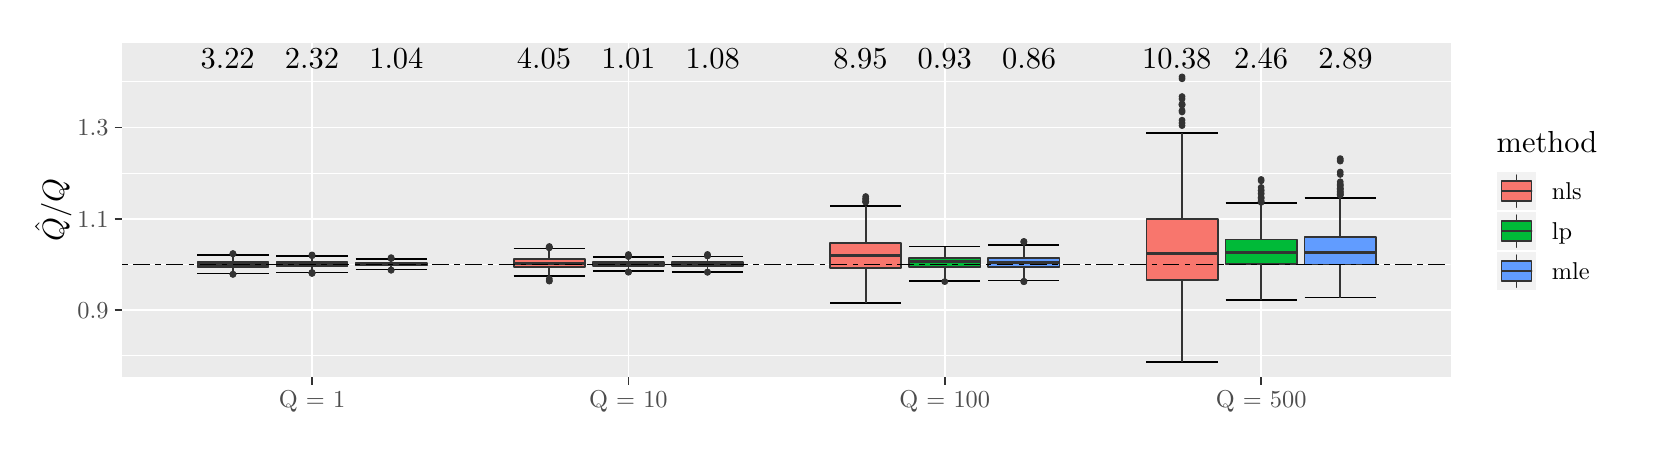
\begin{tikzpicture}[x=1pt,y=1pt]
\definecolor{fillColor}{RGB}{255,255,255}
\path[use as bounding box,fill=fillColor,fill opacity=0.00] (0,0) rectangle (578.16,144.54);
\begin{scope}
\path[clip] (  0.00,  0.00) rectangle (578.16,144.54);
\definecolor{drawColor}{RGB}{255,255,255}
\definecolor{fillColor}{RGB}{255,255,255}

\path[draw=drawColor,line width= 0.6pt,line join=round,line cap=round,fill=fillColor] (  0.00,  0.00) rectangle (578.16,144.54);
\end{scope}
\begin{scope}
\path[clip] ( 34.16, 18.22) rectangle (514.31,139.04);
\definecolor{fillColor}{gray}{0.92}

\path[fill=fillColor] ( 34.16, 18.22) rectangle (514.31,139.04);
\definecolor{drawColor}{RGB}{255,255,255}

\path[draw=drawColor,line width= 0.3pt,line join=round] ( 34.16, 26.06) --
	(514.31, 26.06);

\path[draw=drawColor,line width= 0.3pt,line join=round] ( 34.16, 59.02) --
	(514.31, 59.02);

\path[draw=drawColor,line width= 0.3pt,line join=round] ( 34.16, 91.98) --
	(514.31, 91.98);

\path[draw=drawColor,line width= 0.3pt,line join=round] ( 34.16,124.94) --
	(514.31,124.94);

\path[draw=drawColor,line width= 0.6pt,line join=round] ( 34.16, 42.54) --
	(514.31, 42.54);

\path[draw=drawColor,line width= 0.6pt,line join=round] ( 34.16, 75.50) --
	(514.31, 75.50);

\path[draw=drawColor,line width= 0.6pt,line join=round] ( 34.16,108.46) --
	(514.31,108.46);

\path[draw=drawColor,line width= 0.6pt,line join=round] (102.75, 18.22) --
	(102.75,139.04);

\path[draw=drawColor,line width= 0.6pt,line join=round] (217.07, 18.22) --
	(217.07,139.04);

\path[draw=drawColor,line width= 0.6pt,line join=round] (331.39, 18.22) --
	(331.39,139.04);

\path[draw=drawColor,line width= 0.6pt,line join=round] (445.71, 18.22) --
	(445.71,139.04);
\definecolor{drawColor}{RGB}{0,0,0}

\path[draw=drawColor,line width= 0.6pt,line join=round] ( 61.31, 62.51) --
	( 87.03, 62.51);

\path[draw=drawColor,line width= 0.6pt,line join=round] ( 74.17, 62.51) --
	( 74.17, 55.75);

\path[draw=drawColor,line width= 0.6pt,line join=round] ( 61.31, 55.75) --
	( 87.03, 55.75);

\path[draw=drawColor,line width= 0.6pt,line join=round] ( 89.89, 61.97) --
	(115.61, 61.97);

\path[draw=drawColor,line width= 0.6pt,line join=round] (102.75, 61.97) --
	(102.75, 56.12);

\path[draw=drawColor,line width= 0.6pt,line join=round] ( 89.89, 56.12) --
	(115.61, 56.12);

\path[draw=drawColor,line width= 0.6pt,line join=round] (118.47, 60.94) --
	(144.19, 60.94);

\path[draw=drawColor,line width= 0.6pt,line join=round] (131.33, 60.94) --
	(131.33, 57.10);

\path[draw=drawColor,line width= 0.6pt,line join=round] (118.47, 57.10) --
	(144.19, 57.10);

\path[draw=drawColor,line width= 0.6pt,line join=round] (175.63, 64.79) --
	(201.35, 64.79);

\path[draw=drawColor,line width= 0.6pt,line join=round] (188.49, 64.79) --
	(188.49, 54.70);

\path[draw=drawColor,line width= 0.6pt,line join=round] (175.63, 54.70) --
	(201.35, 54.70);

\path[draw=drawColor,line width= 0.6pt,line join=round] (204.21, 61.71) --
	(229.93, 61.71);

\path[draw=drawColor,line width= 0.6pt,line join=round] (217.07, 61.71) --
	(217.07, 56.61);

\path[draw=drawColor,line width= 0.6pt,line join=round] (204.21, 56.61) --
	(229.93, 56.61);

\path[draw=drawColor,line width= 0.6pt,line join=round] (232.79, 61.90) --
	(258.51, 61.90);

\path[draw=drawColor,line width= 0.6pt,line join=round] (245.65, 61.90) --
	(245.65, 56.37);

\path[draw=drawColor,line width= 0.6pt,line join=round] (232.79, 56.37) --
	(258.51, 56.37);

\path[draw=drawColor,line width= 0.6pt,line join=round] (289.95, 80.09) --
	(315.67, 80.09);

\path[draw=drawColor,line width= 0.6pt,line join=round] (302.81, 80.09) --
	(302.81, 45.07);

\path[draw=drawColor,line width= 0.6pt,line join=round] (289.95, 45.07) --
	(315.67, 45.07);

\path[draw=drawColor,line width= 0.6pt,line join=round] (318.53, 65.42) --
	(344.25, 65.42);

\path[draw=drawColor,line width= 0.6pt,line join=round] (331.39, 65.42) --
	(331.39, 52.97);

\path[draw=drawColor,line width= 0.6pt,line join=round] (318.53, 52.97) --
	(344.25, 52.97);

\path[draw=drawColor,line width= 0.6pt,line join=round] (347.11, 65.96) --
	(372.83, 65.96);

\path[draw=drawColor,line width= 0.6pt,line join=round] (359.97, 65.96) --
	(359.97, 53.24);

\path[draw=drawColor,line width= 0.6pt,line join=round] (347.11, 53.24) --
	(372.83, 53.24);

\path[draw=drawColor,line width= 0.6pt,line join=round] (404.27,106.49) --
	(430.00,106.49);

\path[draw=drawColor,line width= 0.6pt,line join=round] (417.13,106.49) --
	(417.13, 23.71);

\path[draw=drawColor,line width= 0.6pt,line join=round] (404.27, 23.71) --
	(430.00, 23.71);

\path[draw=drawColor,line width= 0.6pt,line join=round] (432.85, 81.29) --
	(458.58, 81.29);

\path[draw=drawColor,line width= 0.6pt,line join=round] (445.71, 81.29) --
	(445.71, 46.19);

\path[draw=drawColor,line width= 0.6pt,line join=round] (432.85, 46.19) --
	(458.58, 46.19);

\path[draw=drawColor,line width= 0.6pt,line join=round] (461.43, 82.95) --
	(487.16, 82.95);

\path[draw=drawColor,line width= 0.6pt,line join=round] (474.29, 82.95) --
	(474.29, 46.99);

\path[draw=drawColor,line width= 0.6pt,line join=round] (461.43, 46.99) --
	(487.16, 46.99);
\definecolor{drawColor}{gray}{0.20}
\definecolor{fillColor}{gray}{0.20}

\path[draw=drawColor,line width= 0.4pt,line join=round,line cap=round,fill=fillColor] ( 74.17, 62.92) circle (  1.02);

\path[draw=drawColor,line width= 0.4pt,line join=round,line cap=round,fill=fillColor] ( 74.17, 55.43) circle (  1.02);

\path[draw=drawColor,line width= 0.4pt,line join=round,line cap=round,fill=fillColor] ( 74.17, 55.42) circle (  1.02);

\path[draw=drawColor,line width= 0.4pt,line join=round,line cap=round,fill=fillColor] ( 74.17, 62.80) circle (  1.02);

\path[draw=drawColor,line width= 0.6pt,line join=round] ( 74.17, 59.88) -- ( 74.17, 62.51);

\path[draw=drawColor,line width= 0.6pt,line join=round] ( 74.17, 58.12) -- ( 74.17, 55.75);
\definecolor{fillColor}{RGB}{248,118,109}

\path[draw=drawColor,line width= 0.6pt,line join=round,line cap=round,fill=fillColor] ( 61.31, 59.88) --
	( 61.31, 58.12) --
	( 87.03, 58.12) --
	( 87.03, 59.88) --
	( 61.31, 59.88) --
	cycle;

\path[draw=drawColor,line width= 1.1pt,line join=round] ( 61.31, 58.96) -- ( 87.03, 58.96);
\definecolor{fillColor}{gray}{0.20}

\path[draw=drawColor,line width= 0.4pt,line join=round,line cap=round,fill=fillColor] (102.75, 56.06) circle (  1.02);

\path[draw=drawColor,line width= 0.4pt,line join=round,line cap=round,fill=fillColor] (102.75, 55.96) circle (  1.02);

\path[draw=drawColor,line width= 0.4pt,line join=round,line cap=round,fill=fillColor] (102.75, 62.12) circle (  1.02);

\path[draw=drawColor,line width= 0.4pt,line join=round,line cap=round,fill=fillColor] (102.75, 62.43) circle (  1.02);

\path[draw=drawColor,line width= 0.4pt,line join=round,line cap=round,fill=fillColor] (102.75, 55.72) circle (  1.02);

\path[draw=drawColor,line width= 0.4pt,line join=round,line cap=round,fill=fillColor] (102.75, 55.92) circle (  1.02);

\path[draw=drawColor,line width= 0.6pt,line join=round] (102.75, 59.76) -- (102.75, 61.97);

\path[draw=drawColor,line width= 0.6pt,line join=round] (102.75, 58.29) -- (102.75, 56.12);
\definecolor{fillColor}{RGB}{0,186,56}

\path[draw=drawColor,line width= 0.6pt,line join=round,line cap=round,fill=fillColor] ( 89.89, 59.76) --
	( 89.89, 58.29) --
	(115.61, 58.29) --
	(115.61, 59.76) --
	( 89.89, 59.76) --
	cycle;

\path[draw=drawColor,line width= 1.1pt,line join=round] ( 89.89, 59.02) -- (115.61, 59.02);
\definecolor{fillColor}{gray}{0.20}

\path[draw=drawColor,line width= 0.4pt,line join=round,line cap=round,fill=fillColor] (131.33, 56.97) circle (  1.02);

\path[draw=drawColor,line width= 0.4pt,line join=round,line cap=round,fill=fillColor] (131.33, 61.45) circle (  1.02);

\path[draw=drawColor,line width= 0.4pt,line join=round,line cap=round,fill=fillColor] (131.33, 61.13) circle (  1.02);

\path[draw=drawColor,line width= 0.4pt,line join=round,line cap=round,fill=fillColor] (131.33, 61.17) circle (  1.02);

\path[draw=drawColor,line width= 0.4pt,line join=round,line cap=round,fill=fillColor] (131.33, 56.90) circle (  1.02);

\path[draw=drawColor,line width= 0.6pt,line join=round] (131.33, 59.52) -- (131.33, 60.94);

\path[draw=drawColor,line width= 0.6pt,line join=round] (131.33, 58.54) -- (131.33, 57.10);
\definecolor{fillColor}{RGB}{97,156,255}

\path[draw=drawColor,line width= 0.6pt,line join=round,line cap=round,fill=fillColor] (118.47, 59.52) --
	(118.47, 58.54) --
	(144.19, 58.54) --
	(144.19, 59.52) --
	(118.47, 59.52) --
	cycle;

\path[draw=drawColor,line width= 1.1pt,line join=round] (118.47, 59.02) -- (144.19, 59.02);
\definecolor{fillColor}{gray}{0.20}

\path[draw=drawColor,line width= 0.4pt,line join=round,line cap=round,fill=fillColor] (188.49, 52.98) circle (  1.02);

\path[draw=drawColor,line width= 0.4pt,line join=round,line cap=round,fill=fillColor] (188.49, 65.06) circle (  1.02);

\path[draw=drawColor,line width= 0.4pt,line join=round,line cap=round,fill=fillColor] (188.49, 65.18) circle (  1.02);

\path[draw=drawColor,line width= 0.4pt,line join=round,line cap=round,fill=fillColor] (188.49, 53.04) circle (  1.02);

\path[draw=drawColor,line width= 0.4pt,line join=round,line cap=round,fill=fillColor] (188.49, 53.80) circle (  1.02);

\path[draw=drawColor,line width= 0.4pt,line join=round,line cap=round,fill=fillColor] (188.49, 65.47) circle (  1.02);

\path[draw=drawColor,line width= 0.4pt,line join=round,line cap=round,fill=fillColor] (188.49, 65.02) circle (  1.02);

\path[draw=drawColor,line width= 0.6pt,line join=round] (188.49, 60.84) -- (188.49, 64.79);

\path[draw=drawColor,line width= 0.6pt,line join=round] (188.49, 58.14) -- (188.49, 54.70);
\definecolor{fillColor}{RGB}{248,118,109}

\path[draw=drawColor,line width= 0.6pt,line join=round,line cap=round,fill=fillColor] (175.63, 60.84) --
	(175.63, 58.14) --
	(201.35, 58.14) --
	(201.35, 60.84) --
	(175.63, 60.84) --
	cycle;

\path[draw=drawColor,line width= 1.1pt,line join=round] (175.63, 59.47) -- (201.35, 59.47);
\definecolor{fillColor}{gray}{0.20}

\path[draw=drawColor,line width= 0.4pt,line join=round,line cap=round,fill=fillColor] (217.07, 56.30) circle (  1.02);

\path[draw=drawColor,line width= 0.4pt,line join=round,line cap=round,fill=fillColor] (217.07, 62.03) circle (  1.02);

\path[draw=drawColor,line width= 0.4pt,line join=round,line cap=round,fill=fillColor] (217.07, 56.20) circle (  1.02);

\path[draw=drawColor,line width= 0.4pt,line join=round,line cap=round,fill=fillColor] (217.07, 62.07) circle (  1.02);

\path[draw=drawColor,line width= 0.4pt,line join=round,line cap=round,fill=fillColor] (217.07, 56.24) circle (  1.02);

\path[draw=drawColor,line width= 0.4pt,line join=round,line cap=round,fill=fillColor] (217.07, 62.00) circle (  1.02);

\path[draw=drawColor,line width= 0.4pt,line join=round,line cap=round,fill=fillColor] (217.07, 62.56) circle (  1.02);

\path[draw=drawColor,line width= 0.4pt,line join=round,line cap=round,fill=fillColor] (217.07, 61.85) circle (  1.02);

\path[draw=drawColor,line width= 0.4pt,line join=round,line cap=round,fill=fillColor] (217.07, 61.98) circle (  1.02);

\path[draw=drawColor,line width= 0.4pt,line join=round,line cap=round,fill=fillColor] (217.07, 62.08) circle (  1.02);

\path[draw=drawColor,line width= 0.6pt,line join=round] (217.07, 59.78) -- (217.07, 61.71);

\path[draw=drawColor,line width= 0.6pt,line join=round] (217.07, 58.45) -- (217.07, 56.61);
\definecolor{fillColor}{RGB}{0,186,56}

\path[draw=drawColor,line width= 0.6pt,line join=round,line cap=round,fill=fillColor] (204.21, 59.78) --
	(204.21, 58.45) --
	(229.93, 58.45) --
	(229.93, 59.78) --
	(204.21, 59.78) --
	cycle;

\path[draw=drawColor,line width= 1.1pt,line join=round] (204.21, 59.11) -- (229.93, 59.11);
\definecolor{fillColor}{gray}{0.20}

\path[draw=drawColor,line width= 0.4pt,line join=round,line cap=round,fill=fillColor] (245.65, 56.23) circle (  1.02);

\path[draw=drawColor,line width= 0.4pt,line join=round,line cap=round,fill=fillColor] (245.65, 56.15) circle (  1.02);

\path[draw=drawColor,line width= 0.4pt,line join=round,line cap=round,fill=fillColor] (245.65, 62.11) circle (  1.02);

\path[draw=drawColor,line width= 0.4pt,line join=round,line cap=round,fill=fillColor] (245.65, 62.59) circle (  1.02);

\path[draw=drawColor,line width= 0.4pt,line join=round,line cap=round,fill=fillColor] (245.65, 62.18) circle (  1.02);

\path[draw=drawColor,line width= 0.4pt,line join=round,line cap=round,fill=fillColor] (245.65, 62.12) circle (  1.02);

\path[draw=drawColor,line width= 0.6pt,line join=round] (245.65, 59.81) -- (245.65, 61.90);

\path[draw=drawColor,line width= 0.6pt,line join=round] (245.65, 58.41) -- (245.65, 56.37);
\definecolor{fillColor}{RGB}{97,156,255}

\path[draw=drawColor,line width= 0.6pt,line join=round,line cap=round,fill=fillColor] (232.79, 59.81) --
	(232.79, 58.41) --
	(258.51, 58.41) --
	(258.51, 59.81) --
	(232.79, 59.81) --
	cycle;

\path[draw=drawColor,line width= 1.1pt,line join=round] (232.79, 59.10) -- (258.51, 59.10);
\definecolor{fillColor}{gray}{0.20}

\path[draw=drawColor,line width= 0.4pt,line join=round,line cap=round,fill=fillColor] (302.81, 81.48) circle (  1.02);

\path[draw=drawColor,line width= 0.4pt,line join=round,line cap=round,fill=fillColor] (302.81, 83.52) circle (  1.02);

\path[draw=drawColor,line width= 0.4pt,line join=round,line cap=round,fill=fillColor] (302.81, 82.78) circle (  1.02);

\path[draw=drawColor,line width= 0.4pt,line join=round,line cap=round,fill=fillColor] (302.81, 81.74) circle (  1.02);

\path[draw=drawColor,line width= 0.4pt,line join=round,line cap=round,fill=fillColor] (302.81, 81.76) circle (  1.02);

\path[draw=drawColor,line width= 0.4pt,line join=round,line cap=round,fill=fillColor] (302.81, 82.57) circle (  1.02);

\path[draw=drawColor,line width= 0.6pt,line join=round] (302.81, 66.80) -- (302.81, 80.09);

\path[draw=drawColor,line width= 0.6pt,line join=round] (302.81, 57.80) -- (302.81, 45.07);
\definecolor{fillColor}{RGB}{248,118,109}

\path[draw=drawColor,line width= 0.6pt,line join=round,line cap=round,fill=fillColor] (289.95, 66.80) --
	(289.95, 57.80) --
	(315.67, 57.80) --
	(315.67, 66.80) --
	(289.95, 66.80) --
	cycle;

\path[draw=drawColor,line width= 1.1pt,line join=round] (289.95, 62.21) -- (315.67, 62.21);
\definecolor{fillColor}{gray}{0.20}

\path[draw=drawColor,line width= 0.4pt,line join=round,line cap=round,fill=fillColor] (331.39, 52.78) circle (  1.02);

\path[draw=drawColor,line width= 0.6pt,line join=round] (331.39, 61.40) -- (331.39, 65.42);

\path[draw=drawColor,line width= 0.6pt,line join=round] (331.39, 58.00) -- (331.39, 52.97);
\definecolor{fillColor}{RGB}{0,186,56}

\path[draw=drawColor,line width= 0.6pt,line join=round,line cap=round,fill=fillColor] (318.53, 61.40) --
	(318.53, 58.00) --
	(344.25, 58.00) --
	(344.25, 61.40) --
	(318.53, 61.40) --
	cycle;

\path[draw=drawColor,line width= 1.1pt,line join=round] (318.53, 59.89) -- (344.25, 59.89);
\definecolor{fillColor}{gray}{0.20}

\path[draw=drawColor,line width= 0.4pt,line join=round,line cap=round,fill=fillColor] (359.97, 67.10) circle (  1.02);

\path[draw=drawColor,line width= 0.4pt,line join=round,line cap=round,fill=fillColor] (359.97, 52.74) circle (  1.02);

\path[draw=drawColor,line width= 0.4pt,line join=round,line cap=round,fill=fillColor] (359.97, 52.85) circle (  1.02);

\path[draw=drawColor,line width= 0.4pt,line join=round,line cap=round,fill=fillColor] (359.97, 52.87) circle (  1.02);

\path[draw=drawColor,line width= 0.4pt,line join=round,line cap=round,fill=fillColor] (359.97, 67.25) circle (  1.02);

\path[draw=drawColor,line width= 0.4pt,line join=round,line cap=round,fill=fillColor] (359.97, 67.26) circle (  1.02);

\path[draw=drawColor,line width= 0.6pt,line join=round] (359.97, 61.21) -- (359.97, 65.96);

\path[draw=drawColor,line width= 0.6pt,line join=round] (359.97, 58.00) -- (359.97, 53.24);
\definecolor{fillColor}{RGB}{97,156,255}

\path[draw=drawColor,line width= 0.6pt,line join=round,line cap=round,fill=fillColor] (347.11, 61.21) --
	(347.11, 58.00) --
	(372.83, 58.00) --
	(372.83, 61.21) --
	(347.11, 61.21) --
	cycle;

\path[draw=drawColor,line width= 1.1pt,line join=round] (347.11, 59.60) -- (372.83, 59.60);
\definecolor{fillColor}{gray}{0.20}

\path[draw=drawColor,line width= 0.4pt,line join=round,line cap=round,fill=fillColor] (417.13,119.65) circle (  1.02);

\path[draw=drawColor,line width= 0.4pt,line join=round,line cap=round,fill=fillColor] (417.13,114.08) circle (  1.02);

\path[draw=drawColor,line width= 0.4pt,line join=round,line cap=round,fill=fillColor] (417.13,110.09) circle (  1.02);

\path[draw=drawColor,line width= 0.4pt,line join=round,line cap=round,fill=fillColor] (417.13,126.07) circle (  1.02);

\path[draw=drawColor,line width= 0.4pt,line join=round,line cap=round,fill=fillColor] (417.13,118.81) circle (  1.02);

\path[draw=drawColor,line width= 0.4pt,line join=round,line cap=round,fill=fillColor] (417.13,116.59) circle (  1.02);

\path[draw=drawColor,line width= 0.4pt,line join=round,line cap=round,fill=fillColor] (417.13,109.16) circle (  1.02);

\path[draw=drawColor,line width= 0.4pt,line join=round,line cap=round,fill=fillColor] (417.13,117.02) circle (  1.02);

\path[draw=drawColor,line width= 0.4pt,line join=round,line cap=round,fill=fillColor] (417.13,111.11) circle (  1.02);

\path[draw=drawColor,line width= 0.4pt,line join=round,line cap=round,fill=fillColor] (417.13,116.72) circle (  1.02);

\path[draw=drawColor,line width= 0.4pt,line join=round,line cap=round,fill=fillColor] (417.13,114.61) circle (  1.02);

\path[draw=drawColor,line width= 0.4pt,line join=round,line cap=round,fill=fillColor] (417.13,126.77) circle (  1.02);

\path[draw=drawColor,line width= 0.6pt,line join=round] (417.13, 75.44) -- (417.13,106.49);

\path[draw=drawColor,line width= 0.6pt,line join=round] (417.13, 53.38) -- (417.13, 23.71);
\definecolor{fillColor}{RGB}{248,118,109}

\path[draw=drawColor,line width= 0.6pt,line join=round,line cap=round,fill=fillColor] (404.27, 75.44) --
	(404.27, 53.38) --
	(430.00, 53.38) --
	(430.00, 75.44) --
	(404.27, 75.44) --
	cycle;

\path[draw=drawColor,line width= 1.1pt,line join=round] (404.27, 62.80) -- (430.00, 62.80);
\definecolor{fillColor}{gray}{0.20}

\path[draw=drawColor,line width= 0.4pt,line join=round,line cap=round,fill=fillColor] (445.71, 84.71) circle (  1.02);

\path[draw=drawColor,line width= 0.4pt,line join=round,line cap=round,fill=fillColor] (445.71, 83.23) circle (  1.02);

\path[draw=drawColor,line width= 0.4pt,line join=round,line cap=round,fill=fillColor] (445.71, 86.82) circle (  1.02);

\path[draw=drawColor,line width= 0.4pt,line join=round,line cap=round,fill=fillColor] (445.71, 81.42) circle (  1.02);

\path[draw=drawColor,line width= 0.4pt,line join=round,line cap=round,fill=fillColor] (445.71, 81.83) circle (  1.02);

\path[draw=drawColor,line width= 0.4pt,line join=round,line cap=round,fill=fillColor] (445.71, 83.08) circle (  1.02);

\path[draw=drawColor,line width= 0.4pt,line join=round,line cap=round,fill=fillColor] (445.71, 82.77) circle (  1.02);

\path[draw=drawColor,line width= 0.4pt,line join=round,line cap=round,fill=fillColor] (445.71, 89.68) circle (  1.02);

\path[draw=drawColor,line width= 0.4pt,line join=round,line cap=round,fill=fillColor] (445.71, 85.80) circle (  1.02);

\path[draw=drawColor,line width= 0.4pt,line join=round,line cap=round,fill=fillColor] (445.71, 84.46) circle (  1.02);

\path[draw=drawColor,line width= 0.4pt,line join=round,line cap=round,fill=fillColor] (445.71, 89.21) circle (  1.02);

\path[draw=drawColor,line width= 0.4pt,line join=round,line cap=round,fill=fillColor] (445.71, 81.77) circle (  1.02);

\path[draw=drawColor,line width= 0.4pt,line join=round,line cap=round,fill=fillColor] (445.71, 85.64) circle (  1.02);

\path[draw=drawColor,line width= 0.6pt,line join=round] (445.71, 68.02) -- (445.71, 81.29);

\path[draw=drawColor,line width= 0.6pt,line join=round] (445.71, 59.17) -- (445.71, 46.19);
\definecolor{fillColor}{RGB}{0,186,56}

\path[draw=drawColor,line width= 0.6pt,line join=round,line cap=round,fill=fillColor] (432.85, 68.02) --
	(432.85, 59.17) --
	(458.58, 59.17) --
	(458.58, 68.02) --
	(432.85, 68.02) --
	cycle;

\path[draw=drawColor,line width= 1.1pt,line join=round] (432.85, 63.14) -- (458.58, 63.14);
\definecolor{fillColor}{gray}{0.20}

\path[draw=drawColor,line width= 0.4pt,line join=round,line cap=round,fill=fillColor] (474.29, 96.31) circle (  1.02);

\path[draw=drawColor,line width= 0.4pt,line join=round,line cap=round,fill=fillColor] (474.29, 84.73) circle (  1.02);

\path[draw=drawColor,line width= 0.4pt,line join=round,line cap=round,fill=fillColor] (474.29, 85.52) circle (  1.02);

\path[draw=drawColor,line width= 0.4pt,line join=round,line cap=round,fill=fillColor] (474.29, 84.88) circle (  1.02);

\path[draw=drawColor,line width= 0.4pt,line join=round,line cap=round,fill=fillColor] (474.29, 87.32) circle (  1.02);

\path[draw=drawColor,line width= 0.4pt,line join=round,line cap=round,fill=fillColor] (474.29, 86.39) circle (  1.02);

\path[draw=drawColor,line width= 0.4pt,line join=round,line cap=round,fill=fillColor] (474.29, 85.32) circle (  1.02);

\path[draw=drawColor,line width= 0.4pt,line join=round,line cap=round,fill=fillColor] (474.29, 86.55) circle (  1.02);

\path[draw=drawColor,line width= 0.4pt,line join=round,line cap=round,fill=fillColor] (474.29, 88.84) circle (  1.02);

\path[draw=drawColor,line width= 0.4pt,line join=round,line cap=round,fill=fillColor] (474.29, 91.50) circle (  1.02);

\path[draw=drawColor,line width= 0.4pt,line join=round,line cap=round,fill=fillColor] (474.29, 96.70) circle (  1.02);

\path[draw=drawColor,line width= 0.4pt,line join=round,line cap=round,fill=fillColor] (474.29, 84.16) circle (  1.02);

\path[draw=drawColor,line width= 0.4pt,line join=round,line cap=round,fill=fillColor] (474.29, 84.06) circle (  1.02);

\path[draw=drawColor,line width= 0.4pt,line join=round,line cap=round,fill=fillColor] (474.29, 92.38) circle (  1.02);

\path[draw=drawColor,line width= 0.4pt,line join=round,line cap=round,fill=fillColor] (474.29, 97.23) circle (  1.02);

\path[draw=drawColor,line width= 0.4pt,line join=round,line cap=round,fill=fillColor] (474.29, 86.10) circle (  1.02);

\path[draw=drawColor,line width= 0.4pt,line join=round,line cap=round,fill=fillColor] (474.29, 84.14) circle (  1.02);

\path[draw=drawColor,line width= 0.4pt,line join=round,line cap=round,fill=fillColor] (474.29, 87.63) circle (  1.02);

\path[draw=drawColor,line width= 0.4pt,line join=round,line cap=round,fill=fillColor] (474.29, 88.01) circle (  1.02);

\path[draw=drawColor,line width= 0.6pt,line join=round] (474.29, 68.91) -- (474.29, 82.95);

\path[draw=drawColor,line width= 0.6pt,line join=round] (474.29, 59.02) -- (474.29, 46.99);
\definecolor{fillColor}{RGB}{97,156,255}

\path[draw=drawColor,line width= 0.6pt,line join=round,line cap=round,fill=fillColor] (461.43, 68.91) --
	(461.43, 59.02) --
	(487.16, 59.02) --
	(487.16, 68.91) --
	(461.43, 68.91) --
	cycle;

\path[draw=drawColor,line width= 1.1pt,line join=round] (461.43, 63.29) -- (487.16, 63.29);
\definecolor{drawColor}{RGB}{0,0,0}

\path[draw=drawColor,line width= 0.6pt,dash pattern=on 2pt off 2pt on 6pt off 2pt ,line join=round] ( 34.16, 59.02) -- (514.31, 59.02);

\node[text=drawColor,anchor=base,inner sep=0pt, outer sep=0pt, scale=  1.10] at (133.23,129.75) {1.04};

\node[text=drawColor,anchor=base,inner sep=0pt, outer sep=0pt, scale=  1.10] at (102.75,129.75) {2.32};

\node[text=drawColor,anchor=base,inner sep=0pt, outer sep=0pt, scale=  1.10] at ( 72.26,129.75) {3.22};

\node[text=drawColor,anchor=base,inner sep=0pt, outer sep=0pt, scale=  1.10] at (247.56,129.75) {1.08};

\node[text=drawColor,anchor=base,inner sep=0pt, outer sep=0pt, scale=  1.10] at (217.07,129.75) {1.01};

\node[text=drawColor,anchor=base,inner sep=0pt, outer sep=0pt, scale=  1.10] at (186.59,129.75) {4.05};

\node[text=drawColor,anchor=base,inner sep=0pt, outer sep=0pt, scale=  1.10] at (361.88,129.75) {0.86};

\node[text=drawColor,anchor=base,inner sep=0pt, outer sep=0pt, scale=  1.10] at (331.39,129.75) {0.93};

\node[text=drawColor,anchor=base,inner sep=0pt, outer sep=0pt, scale=  1.10] at (300.91,129.75) {8.95};

\node[text=drawColor,anchor=base,inner sep=0pt, outer sep=0pt, scale=  1.10] at (476.20,129.75) {2.89};

\node[text=drawColor,anchor=base,inner sep=0pt, outer sep=0pt, scale=  1.10] at (445.71,129.75) {2.46};

\node[text=drawColor,anchor=base,inner sep=0pt, outer sep=0pt, scale=  1.10] at (415.23,129.75) {10.38};
\end{scope}
\begin{scope}
\path[clip] (  0.00,  0.00) rectangle (578.16,144.54);
\definecolor{drawColor}{gray}{0.30}

\node[text=drawColor,anchor=base east,inner sep=0pt, outer sep=0pt, scale=  0.88] at ( 29.21, 39.51) {0.9};

\node[text=drawColor,anchor=base east,inner sep=0pt, outer sep=0pt, scale=  0.88] at ( 29.21, 72.47) {1.1};

\node[text=drawColor,anchor=base east,inner sep=0pt, outer sep=0pt, scale=  0.88] at ( 29.21,105.43) {1.3};
\end{scope}
\begin{scope}
\path[clip] (  0.00,  0.00) rectangle (578.16,144.54);
\definecolor{drawColor}{gray}{0.20}

\path[draw=drawColor,line width= 0.6pt,line join=round] ( 31.41, 42.54) --
	( 34.16, 42.54);

\path[draw=drawColor,line width= 0.6pt,line join=round] ( 31.41, 75.50) --
	( 34.16, 75.50);

\path[draw=drawColor,line width= 0.6pt,line join=round] ( 31.41,108.46) --
	( 34.16,108.46);
\end{scope}
\begin{scope}
\path[clip] (  0.00,  0.00) rectangle (578.16,144.54);
\definecolor{drawColor}{gray}{0.20}

\path[draw=drawColor,line width= 0.6pt,line join=round] (102.75, 15.47) --
	(102.75, 18.22);

\path[draw=drawColor,line width= 0.6pt,line join=round] (217.07, 15.47) --
	(217.07, 18.22);

\path[draw=drawColor,line width= 0.6pt,line join=round] (331.39, 15.47) --
	(331.39, 18.22);

\path[draw=drawColor,line width= 0.6pt,line join=round] (445.71, 15.47) --
	(445.71, 18.22);
\end{scope}
\begin{scope}
\path[clip] (  0.00,  0.00) rectangle (578.16,144.54);
\definecolor{drawColor}{gray}{0.30}

\node[text=drawColor,anchor=base,inner sep=0pt, outer sep=0pt, scale=  0.88] at (102.75,  7.21) {Q = 1};

\node[text=drawColor,anchor=base,inner sep=0pt, outer sep=0pt, scale=  0.88] at (217.07,  7.21) {Q = 10};

\node[text=drawColor,anchor=base,inner sep=0pt, outer sep=0pt, scale=  0.88] at (331.39,  7.21) {Q = 100};

\node[text=drawColor,anchor=base,inner sep=0pt, outer sep=0pt, scale=  0.88] at (445.71,  7.21) {Q = 500};
\end{scope}
\begin{scope}
\path[clip] (  0.00,  0.00) rectangle (578.16,144.54);
\definecolor{drawColor}{RGB}{0,0,0}

\node[text=drawColor,rotate= 90.00,anchor=base,inner sep=0pt, outer sep=0pt, scale=  1.10] at ( 13.08, 78.63) {$\hat{Q}/Q$};
\end{scope}
\begin{scope}
\path[clip] (  0.00,  0.00) rectangle (578.16,144.54);
\definecolor{fillColor}{RGB}{255,255,255}

\path[fill=fillColor] (525.31, 43.84) rectangle (572.66,113.42);
\end{scope}
\begin{scope}
\path[clip] (  0.00,  0.00) rectangle (578.16,144.54);
\definecolor{drawColor}{RGB}{0,0,0}

\node[text=drawColor,anchor=base west,inner sep=0pt, outer sep=0pt, scale=  1.10] at (530.81, 99.27) {method};
\end{scope}
\begin{scope}
\path[clip] (  0.00,  0.00) rectangle (578.16,144.54);
\definecolor{drawColor}{RGB}{255,255,255}
\definecolor{fillColor}{gray}{0.95}

\path[draw=drawColor,line width= 0.6pt,line join=round,line cap=round,fill=fillColor] (530.81, 78.25) rectangle (545.26, 92.70);
\end{scope}
\begin{scope}
\path[clip] (  0.00,  0.00) rectangle (578.16,144.54);
\definecolor{drawColor}{gray}{0.20}

\path[draw=drawColor,line width= 0.6pt,line join=round,line cap=round] (538.03, 79.70) --
	(538.03, 81.86);

\path[draw=drawColor,line width= 0.6pt,line join=round,line cap=round] (538.03, 89.09) --
	(538.03, 91.26);
\definecolor{fillColor}{RGB}{248,118,109}

\path[draw=drawColor,line width= 0.6pt,line join=round,line cap=round,fill=fillColor] (532.61, 81.86) rectangle (543.45, 89.09);

\path[draw=drawColor,line width= 0.6pt,line join=round,line cap=round] (532.61, 85.48) --
	(543.45, 85.48);
\end{scope}
\begin{scope}
\path[clip] (  0.00,  0.00) rectangle (578.16,144.54);
\definecolor{drawColor}{RGB}{255,255,255}
\definecolor{fillColor}{gray}{0.95}

\path[draw=drawColor,line width= 0.6pt,line join=round,line cap=round,fill=fillColor] (530.81, 63.80) rectangle (545.26, 78.25);
\end{scope}
\begin{scope}
\path[clip] (  0.00,  0.00) rectangle (578.16,144.54);
\definecolor{drawColor}{gray}{0.20}

\path[draw=drawColor,line width= 0.6pt,line join=round,line cap=round] (538.03, 65.24) --
	(538.03, 67.41);

\path[draw=drawColor,line width= 0.6pt,line join=round,line cap=round] (538.03, 74.64) --
	(538.03, 76.81);
\definecolor{fillColor}{RGB}{0,186,56}

\path[draw=drawColor,line width= 0.6pt,line join=round,line cap=round,fill=fillColor] (532.61, 67.41) rectangle (543.45, 74.64);

\path[draw=drawColor,line width= 0.6pt,line join=round,line cap=round] (532.61, 71.02) --
	(543.45, 71.02);
\end{scope}
\begin{scope}
\path[clip] (  0.00,  0.00) rectangle (578.16,144.54);
\definecolor{drawColor}{RGB}{255,255,255}
\definecolor{fillColor}{gray}{0.95}

\path[draw=drawColor,line width= 0.6pt,line join=round,line cap=round,fill=fillColor] (530.81, 49.34) rectangle (545.26, 63.80);
\end{scope}
\begin{scope}
\path[clip] (  0.00,  0.00) rectangle (578.16,144.54);
\definecolor{drawColor}{gray}{0.20}

\path[draw=drawColor,line width= 0.6pt,line join=round,line cap=round] (538.03, 50.79) --
	(538.03, 52.96);

\path[draw=drawColor,line width= 0.6pt,line join=round,line cap=round] (538.03, 60.18) --
	(538.03, 62.35);
\definecolor{fillColor}{RGB}{97,156,255}

\path[draw=drawColor,line width= 0.6pt,line join=round,line cap=round,fill=fillColor] (532.61, 52.96) rectangle (543.45, 60.18);

\path[draw=drawColor,line width= 0.6pt,line join=round,line cap=round] (532.61, 56.57) --
	(543.45, 56.57);
\end{scope}
\begin{scope}
\path[clip] (  0.00,  0.00) rectangle (578.16,144.54);
\definecolor{drawColor}{RGB}{0,0,0}

\node[text=drawColor,anchor=base west,inner sep=0pt, outer sep=0pt, scale=  0.88] at (550.76, 82.45) {nls};
\end{scope}
\begin{scope}
\path[clip] (  0.00,  0.00) rectangle (578.16,144.54);
\definecolor{drawColor}{RGB}{0,0,0}

\node[text=drawColor,anchor=base west,inner sep=0pt, outer sep=0pt, scale=  0.88] at (550.76, 67.99) {lp};
\end{scope}
\begin{scope}
\path[clip] (  0.00,  0.00) rectangle (578.16,144.54);
\definecolor{drawColor}{RGB}{0,0,0}

\node[text=drawColor,anchor=base west,inner sep=0pt, outer sep=0pt, scale=  0.88] at (550.76, 53.54) {mle};
\end{scope}
\end{tikzpicture}
}
%   \end{subfigure}
%   \hfill
%   \begin{subfigure}
%     \centering
%     \resizebox{1.1\linewidth}{!}{% Created by tikzDevice version 0.12.3 on 2019-09-26 18:31:10
% !TEX encoding = UTF-8 Unicode
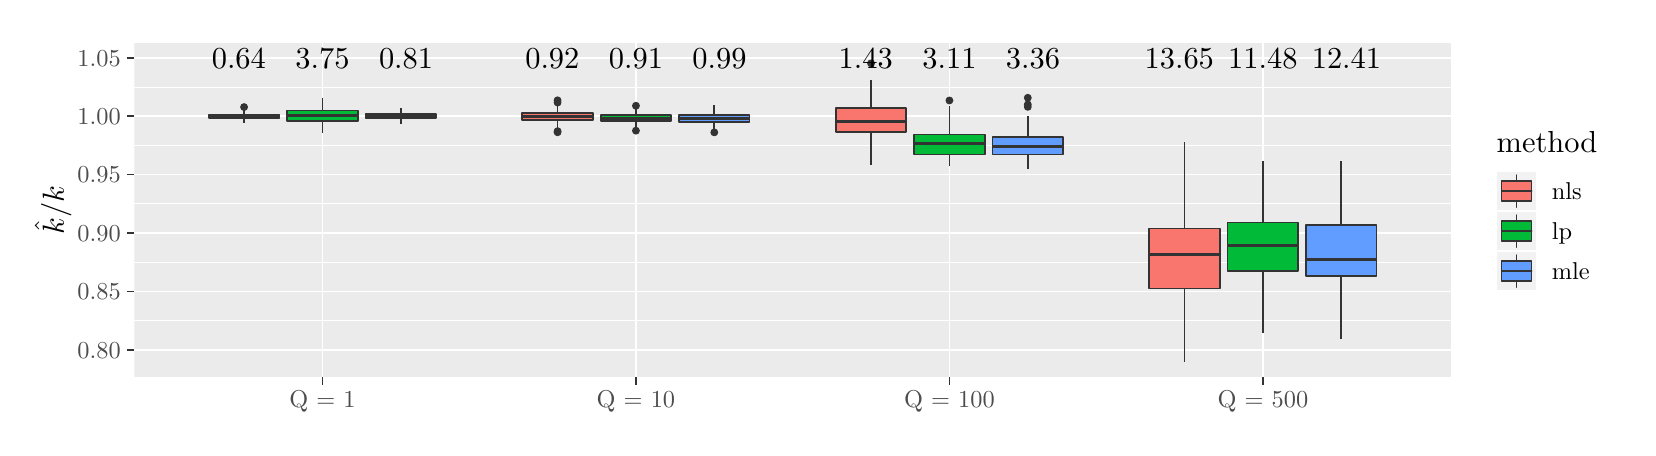
\begin{tikzpicture}[x=1pt,y=1pt]
\definecolor{fillColor}{RGB}{255,255,255}
\path[use as bounding box,fill=fillColor,fill opacity=0.00] (0,0) rectangle (578.16,144.54);
\begin{scope}
\path[clip] (  0.00,  0.00) rectangle (578.16,144.54);
\definecolor{drawColor}{RGB}{255,255,255}
\definecolor{fillColor}{RGB}{255,255,255}

\path[draw=drawColor,line width= 0.6pt,line join=round,line cap=round,fill=fillColor] (  0.00,  0.00) rectangle (578.16,144.54);
\end{scope}
\begin{scope}
\path[clip] ( 38.56, 18.22) rectangle (514.31,139.04);
\definecolor{fillColor}{gray}{0.92}

\path[fill=fillColor] ( 38.56, 18.22) rectangle (514.31,139.04);
\definecolor{drawColor}{RGB}{255,255,255}

\path[draw=drawColor,line width= 0.3pt,line join=round] ( 38.56, 38.69) --
	(514.31, 38.69);

\path[draw=drawColor,line width= 0.3pt,line join=round] ( 38.56, 59.80) --
	(514.31, 59.80);

\path[draw=drawColor,line width= 0.3pt,line join=round] ( 38.56, 80.91) --
	(514.31, 80.91);

\path[draw=drawColor,line width= 0.3pt,line join=round] ( 38.56,102.02) --
	(514.31,102.02);

\path[draw=drawColor,line width= 0.3pt,line join=round] ( 38.56,123.13) --
	(514.31,123.13);

\path[draw=drawColor,line width= 0.6pt,line join=round] ( 38.56, 28.13) --
	(514.31, 28.13);

\path[draw=drawColor,line width= 0.6pt,line join=round] ( 38.56, 49.24) --
	(514.31, 49.24);

\path[draw=drawColor,line width= 0.6pt,line join=round] ( 38.56, 70.35) --
	(514.31, 70.35);

\path[draw=drawColor,line width= 0.6pt,line join=round] ( 38.56, 91.46) --
	(514.31, 91.46);

\path[draw=drawColor,line width= 0.6pt,line join=round] ( 38.56,112.57) --
	(514.31,112.57);

\path[draw=drawColor,line width= 0.6pt,line join=round] ( 38.56,133.68) --
	(514.31,133.68);

\path[draw=drawColor,line width= 0.6pt,line join=round] (106.52, 18.22) --
	(106.52,139.04);

\path[draw=drawColor,line width= 0.6pt,line join=round] (219.79, 18.22) --
	(219.79,139.04);

\path[draw=drawColor,line width= 0.6pt,line join=round] (333.07, 18.22) --
	(333.07,139.04);

\path[draw=drawColor,line width= 0.6pt,line join=round] (446.34, 18.22) --
	(446.34,139.04);
\definecolor{drawColor}{gray}{0.20}
\definecolor{fillColor}{gray}{0.20}

\path[draw=drawColor,line width= 0.4pt,line join=round,line cap=round,fill=fillColor] ( 78.20,115.84) circle (  1.21);

\path[draw=drawColor,line width= 0.6pt,line join=round] ( 78.20,113.16) -- ( 78.20,114.96);

\path[draw=drawColor,line width= 0.6pt,line join=round] ( 78.20,111.95) -- ( 78.20,110.26);
\definecolor{fillColor}{RGB}{248,118,109}

\path[draw=drawColor,line width= 0.6pt,line join=round,line cap=round,fill=fillColor] ( 65.46,113.16) --
	( 65.46,111.95) --
	( 90.94,111.95) --
	( 90.94,113.16) --
	( 65.46,113.16) --
	cycle;

\path[draw=drawColor,line width= 1.1pt,line join=round] ( 65.46,112.53) -- ( 90.94,112.53);

\path[draw=drawColor,line width= 0.6pt,line join=round] (106.52,114.61) -- (106.52,119.28);

\path[draw=drawColor,line width= 0.6pt,line join=round] (106.52,110.92) -- (106.52,106.46);
\definecolor{fillColor}{RGB}{0,186,56}

\path[draw=drawColor,line width= 0.6pt,line join=round,line cap=round,fill=fillColor] ( 93.78,114.61) --
	( 93.78,110.92) --
	(119.26,110.92) --
	(119.26,114.61) --
	( 93.78,114.61) --
	cycle;

\path[draw=drawColor,line width= 1.1pt,line join=round] ( 93.78,112.63) -- (119.26,112.63);

\path[draw=drawColor,line width= 0.6pt,line join=round] (134.84,113.41) -- (134.84,115.64);

\path[draw=drawColor,line width= 0.6pt,line join=round] (134.84,111.90) -- (134.84,109.83);
\definecolor{fillColor}{RGB}{97,156,255}

\path[draw=drawColor,line width= 0.6pt,line join=round,line cap=round,fill=fillColor] (122.09,113.41) --
	(122.09,111.90) --
	(147.58,111.90) --
	(147.58,113.41) --
	(122.09,113.41) --
	cycle;

\path[draw=drawColor,line width= 1.1pt,line join=round] (122.09,112.45) -- (147.58,112.45);
\definecolor{fillColor}{gray}{0.20}

\path[draw=drawColor,line width= 0.4pt,line join=round,line cap=round,fill=fillColor] (191.48,107.14) circle (  1.21);

\path[draw=drawColor,line width= 0.4pt,line join=round,line cap=round,fill=fillColor] (191.48,117.48) circle (  1.21);

\path[draw=drawColor,line width= 0.4pt,line join=round,line cap=round,fill=fillColor] (191.48,106.74) circle (  1.21);

\path[draw=drawColor,line width= 0.4pt,line join=round,line cap=round,fill=fillColor] (191.48,118.29) circle (  1.21);

\path[draw=drawColor,line width= 0.6pt,line join=round] (191.48,113.73) -- (191.48,116.74);

\path[draw=drawColor,line width= 0.6pt,line join=round] (191.48,111.23) -- (191.48,108.12);
\definecolor{fillColor}{RGB}{248,118,109}

\path[draw=drawColor,line width= 0.6pt,line join=round,line cap=round,fill=fillColor] (178.73,113.73) --
	(178.73,111.23) --
	(204.22,111.23) --
	(204.22,113.73) --
	(178.73,113.73) --
	cycle;

\path[draw=drawColor,line width= 1.1pt,line join=round] (178.73,112.55) -- (204.22,112.55);
\definecolor{fillColor}{gray}{0.20}

\path[draw=drawColor,line width= 0.4pt,line join=round,line cap=round,fill=fillColor] (219.79,107.32) circle (  1.21);

\path[draw=drawColor,line width= 0.4pt,line join=round,line cap=round,fill=fillColor] (219.79,116.32) circle (  1.21);

\path[draw=drawColor,line width= 0.6pt,line join=round] (219.79,112.93) -- (219.79,115.54);

\path[draw=drawColor,line width= 0.6pt,line join=round] (219.79,110.73) -- (219.79,107.48);
\definecolor{fillColor}{RGB}{0,186,56}

\path[draw=drawColor,line width= 0.6pt,line join=round,line cap=round,fill=fillColor] (207.05,112.93) --
	(207.05,110.73) --
	(232.54,110.73) --
	(232.54,112.93) --
	(207.05,112.93) --
	cycle;

\path[draw=drawColor,line width= 1.1pt,line join=round] (207.05,111.80) -- (232.54,111.80);
\definecolor{fillColor}{gray}{0.20}

\path[draw=drawColor,line width= 0.4pt,line join=round,line cap=round,fill=fillColor] (248.11,106.71) circle (  1.21);

\path[draw=drawColor,line width= 0.6pt,line join=round] (248.11,112.92) -- (248.11,116.42);

\path[draw=drawColor,line width= 0.6pt,line join=round] (248.11,110.52) -- (248.11,106.99);
\definecolor{fillColor}{RGB}{97,156,255}

\path[draw=drawColor,line width= 0.6pt,line join=round,line cap=round,fill=fillColor] (235.37,112.92) --
	(235.37,110.52) --
	(260.86,110.52) --
	(260.86,112.92) --
	(235.37,112.92) --
	cycle;

\path[draw=drawColor,line width= 1.1pt,line join=round] (235.37,111.89) -- (260.86,111.89);
\definecolor{fillColor}{gray}{0.20}

\path[draw=drawColor,line width= 0.4pt,line join=round,line cap=round,fill=fillColor] (304.75,131.64) circle (  1.21);

\path[draw=drawColor,line width= 0.6pt,line join=round] (304.75,115.44) -- (304.75,125.75);

\path[draw=drawColor,line width= 0.6pt,line join=round] (304.75,106.91) -- (304.75, 94.74);
\definecolor{fillColor}{RGB}{248,118,109}

\path[draw=drawColor,line width= 0.6pt,line join=round,line cap=round,fill=fillColor] (292.01,115.44) --
	(292.01,106.91) --
	(317.49,106.91) --
	(317.49,115.44) --
	(292.01,115.44) --
	cycle;

\path[draw=drawColor,line width= 1.1pt,line join=round] (292.01,110.75) -- (317.49,110.75);
\definecolor{fillColor}{gray}{0.20}

\path[draw=drawColor,line width= 0.4pt,line join=round,line cap=round,fill=fillColor] (333.07,118.23) circle (  1.21);

\path[draw=drawColor,line width= 0.6pt,line join=round] (333.07,105.94) -- (333.07,116.09);

\path[draw=drawColor,line width= 0.6pt,line join=round] (333.07, 98.65) -- (333.07, 94.39);
\definecolor{fillColor}{RGB}{0,186,56}

\path[draw=drawColor,line width= 0.6pt,line join=round,line cap=round,fill=fillColor] (320.33,105.94) --
	(320.33, 98.65) --
	(345.81, 98.65) --
	(345.81,105.94) --
	(320.33,105.94) --
	cycle;

\path[draw=drawColor,line width= 1.1pt,line join=round] (320.33,102.71) -- (345.81,102.71);
\definecolor{fillColor}{gray}{0.20}

\path[draw=drawColor,line width= 0.4pt,line join=round,line cap=round,fill=fillColor] (361.39,115.92) circle (  1.21);

\path[draw=drawColor,line width= 0.4pt,line join=round,line cap=round,fill=fillColor] (361.39,116.80) circle (  1.21);

\path[draw=drawColor,line width= 0.4pt,line join=round,line cap=round,fill=fillColor] (361.39,119.21) circle (  1.21);

\path[draw=drawColor,line width= 0.6pt,line join=round] (361.39,104.95) -- (361.39,112.57);

\path[draw=drawColor,line width= 0.6pt,line join=round] (361.39, 98.75) -- (361.39, 93.57);
\definecolor{fillColor}{RGB}{97,156,255}

\path[draw=drawColor,line width= 0.6pt,line join=round,line cap=round,fill=fillColor] (348.64,104.95) --
	(348.64, 98.75) --
	(374.13, 98.75) --
	(374.13,104.95) --
	(348.64,104.95) --
	cycle;

\path[draw=drawColor,line width= 1.1pt,line join=round] (348.64,101.57) -- (374.13,101.57);

\path[draw=drawColor,line width= 0.6pt,line join=round] (418.02, 71.96) -- (418.02,103.06);

\path[draw=drawColor,line width= 0.6pt,line join=round] (418.02, 50.27) -- (418.02, 23.71);
\definecolor{fillColor}{RGB}{248,118,109}

\path[draw=drawColor,line width= 0.6pt,line join=round,line cap=round,fill=fillColor] (405.28, 71.96) --
	(405.28, 50.27) --
	(430.77, 50.27) --
	(430.77, 71.96) --
	(405.28, 71.96) --
	cycle;

\path[draw=drawColor,line width= 1.1pt,line join=round] (405.28, 62.65) -- (430.77, 62.65);

\path[draw=drawColor,line width= 0.6pt,line join=round] (446.34, 74.14) -- (446.34, 96.48);

\path[draw=drawColor,line width= 0.6pt,line join=round] (446.34, 56.68) -- (446.34, 34.03);
\definecolor{fillColor}{RGB}{0,186,56}

\path[draw=drawColor,line width= 0.6pt,line join=round,line cap=round,fill=fillColor] (433.60, 74.14) --
	(433.60, 56.68) --
	(459.09, 56.68) --
	(459.09, 74.14) --
	(433.60, 74.14) --
	cycle;

\path[draw=drawColor,line width= 1.1pt,line join=round] (433.60, 65.79) -- (459.09, 65.79);

\path[draw=drawColor,line width= 0.6pt,line join=round] (474.66, 73.22) -- (474.66, 96.48);

\path[draw=drawColor,line width= 0.6pt,line join=round] (474.66, 54.72) -- (474.66, 32.20);
\definecolor{fillColor}{RGB}{97,156,255}

\path[draw=drawColor,line width= 0.6pt,line join=round,line cap=round,fill=fillColor] (461.92, 73.22) --
	(461.92, 54.72) --
	(487.40, 54.72) --
	(487.40, 73.22) --
	(461.92, 73.22) --
	cycle;

\path[draw=drawColor,line width= 1.1pt,line join=round] (461.92, 60.83) -- (487.40, 60.83);
\definecolor{drawColor}{RGB}{0,0,0}

\node[text=drawColor,anchor=base,inner sep=0pt, outer sep=0pt, scale=  1.10] at (136.73,129.75) {0.81};

\node[text=drawColor,anchor=base,inner sep=0pt, outer sep=0pt, scale=  1.10] at (106.52,129.75) {3.75};

\node[text=drawColor,anchor=base,inner sep=0pt, outer sep=0pt, scale=  1.10] at ( 76.31,129.75) {0.64};

\node[text=drawColor,anchor=base,inner sep=0pt, outer sep=0pt, scale=  1.10] at (250.00,129.75) {0.99};

\node[text=drawColor,anchor=base,inner sep=0pt, outer sep=0pt, scale=  1.10] at (219.79,129.75) {0.91};

\node[text=drawColor,anchor=base,inner sep=0pt, outer sep=0pt, scale=  1.10] at (189.59,129.75) {0.92};

\node[text=drawColor,anchor=base,inner sep=0pt, outer sep=0pt, scale=  1.10] at (363.28,129.75) {3.36};

\node[text=drawColor,anchor=base,inner sep=0pt, outer sep=0pt, scale=  1.10] at (333.07,129.75) {3.11};

\node[text=drawColor,anchor=base,inner sep=0pt, outer sep=0pt, scale=  1.10] at (302.86,129.75) {1.43};

\node[text=drawColor,anchor=base,inner sep=0pt, outer sep=0pt, scale=  1.10] at (476.55,129.75) {12.41};

\node[text=drawColor,anchor=base,inner sep=0pt, outer sep=0pt, scale=  1.10] at (446.34,129.75) {11.48};

\node[text=drawColor,anchor=base,inner sep=0pt, outer sep=0pt, scale=  1.10] at (416.14,129.75) {13.65};
\end{scope}
\begin{scope}
\path[clip] (  0.00,  0.00) rectangle (578.16,144.54);
\definecolor{drawColor}{gray}{0.30}

\node[text=drawColor,anchor=base east,inner sep=0pt, outer sep=0pt, scale=  0.88] at ( 33.61, 25.10) {0.80};

\node[text=drawColor,anchor=base east,inner sep=0pt, outer sep=0pt, scale=  0.88] at ( 33.61, 46.21) {0.85};

\node[text=drawColor,anchor=base east,inner sep=0pt, outer sep=0pt, scale=  0.88] at ( 33.61, 67.32) {0.90};

\node[text=drawColor,anchor=base east,inner sep=0pt, outer sep=0pt, scale=  0.88] at ( 33.61, 88.43) {0.95};

\node[text=drawColor,anchor=base east,inner sep=0pt, outer sep=0pt, scale=  0.88] at ( 33.61,109.54) {1.00};

\node[text=drawColor,anchor=base east,inner sep=0pt, outer sep=0pt, scale=  0.88] at ( 33.61,130.65) {1.05};
\end{scope}
\begin{scope}
\path[clip] (  0.00,  0.00) rectangle (578.16,144.54);
\definecolor{drawColor}{gray}{0.20}

\path[draw=drawColor,line width= 0.6pt,line join=round] ( 35.81, 28.13) --
	( 38.56, 28.13);

\path[draw=drawColor,line width= 0.6pt,line join=round] ( 35.81, 49.24) --
	( 38.56, 49.24);

\path[draw=drawColor,line width= 0.6pt,line join=round] ( 35.81, 70.35) --
	( 38.56, 70.35);

\path[draw=drawColor,line width= 0.6pt,line join=round] ( 35.81, 91.46) --
	( 38.56, 91.46);

\path[draw=drawColor,line width= 0.6pt,line join=round] ( 35.81,112.57) --
	( 38.56,112.57);

\path[draw=drawColor,line width= 0.6pt,line join=round] ( 35.81,133.68) --
	( 38.56,133.68);
\end{scope}
\begin{scope}
\path[clip] (  0.00,  0.00) rectangle (578.16,144.54);
\definecolor{drawColor}{gray}{0.20}

\path[draw=drawColor,line width= 0.6pt,line join=round] (106.52, 15.47) --
	(106.52, 18.22);

\path[draw=drawColor,line width= 0.6pt,line join=round] (219.79, 15.47) --
	(219.79, 18.22);

\path[draw=drawColor,line width= 0.6pt,line join=round] (333.07, 15.47) --
	(333.07, 18.22);

\path[draw=drawColor,line width= 0.6pt,line join=round] (446.34, 15.47) --
	(446.34, 18.22);
\end{scope}
\begin{scope}
\path[clip] (  0.00,  0.00) rectangle (578.16,144.54);
\definecolor{drawColor}{gray}{0.30}

\node[text=drawColor,anchor=base,inner sep=0pt, outer sep=0pt, scale=  0.88] at (106.52,  7.21) {Q = 1};

\node[text=drawColor,anchor=base,inner sep=0pt, outer sep=0pt, scale=  0.88] at (219.79,  7.21) {Q = 10};

\node[text=drawColor,anchor=base,inner sep=0pt, outer sep=0pt, scale=  0.88] at (333.07,  7.21) {Q = 100};

\node[text=drawColor,anchor=base,inner sep=0pt, outer sep=0pt, scale=  0.88] at (446.34,  7.21) {Q = 500};
\end{scope}
\begin{scope}
\path[clip] (  0.00,  0.00) rectangle (578.16,144.54);
\definecolor{drawColor}{RGB}{0,0,0}

\node[text=drawColor,rotate= 90.00,anchor=base,inner sep=0pt, outer sep=0pt, scale=  1.10] at ( 13.08, 78.63) {$\hat{k}/k$};
\end{scope}
\begin{scope}
\path[clip] (  0.00,  0.00) rectangle (578.16,144.54);
\definecolor{fillColor}{RGB}{255,255,255}

\path[fill=fillColor] (525.31, 43.84) rectangle (572.66,113.42);
\end{scope}
\begin{scope}
\path[clip] (  0.00,  0.00) rectangle (578.16,144.54);
\definecolor{drawColor}{RGB}{0,0,0}

\node[text=drawColor,anchor=base west,inner sep=0pt, outer sep=0pt, scale=  1.10] at (530.81, 99.27) {method};
\end{scope}
\begin{scope}
\path[clip] (  0.00,  0.00) rectangle (578.16,144.54);
\definecolor{drawColor}{RGB}{255,255,255}
\definecolor{fillColor}{gray}{0.95}

\path[draw=drawColor,line width= 0.6pt,line join=round,line cap=round,fill=fillColor] (530.81, 78.25) rectangle (545.26, 92.70);
\end{scope}
\begin{scope}
\path[clip] (  0.00,  0.00) rectangle (578.16,144.54);
\definecolor{drawColor}{gray}{0.20}

\path[draw=drawColor,line width= 0.6pt,line join=round,line cap=round] (538.03, 79.70) --
	(538.03, 81.86);

\path[draw=drawColor,line width= 0.6pt,line join=round,line cap=round] (538.03, 89.09) --
	(538.03, 91.26);
\definecolor{fillColor}{RGB}{248,118,109}

\path[draw=drawColor,line width= 0.6pt,line join=round,line cap=round,fill=fillColor] (532.61, 81.86) rectangle (543.45, 89.09);

\path[draw=drawColor,line width= 0.6pt,line join=round,line cap=round] (532.61, 85.48) --
	(543.45, 85.48);
\end{scope}
\begin{scope}
\path[clip] (  0.00,  0.00) rectangle (578.16,144.54);
\definecolor{drawColor}{RGB}{255,255,255}
\definecolor{fillColor}{gray}{0.95}

\path[draw=drawColor,line width= 0.6pt,line join=round,line cap=round,fill=fillColor] (530.81, 63.80) rectangle (545.26, 78.25);
\end{scope}
\begin{scope}
\path[clip] (  0.00,  0.00) rectangle (578.16,144.54);
\definecolor{drawColor}{gray}{0.20}

\path[draw=drawColor,line width= 0.6pt,line join=round,line cap=round] (538.03, 65.24) --
	(538.03, 67.41);

\path[draw=drawColor,line width= 0.6pt,line join=round,line cap=round] (538.03, 74.64) --
	(538.03, 76.81);
\definecolor{fillColor}{RGB}{0,186,56}

\path[draw=drawColor,line width= 0.6pt,line join=round,line cap=round,fill=fillColor] (532.61, 67.41) rectangle (543.45, 74.64);

\path[draw=drawColor,line width= 0.6pt,line join=round,line cap=round] (532.61, 71.02) --
	(543.45, 71.02);
\end{scope}
\begin{scope}
\path[clip] (  0.00,  0.00) rectangle (578.16,144.54);
\definecolor{drawColor}{RGB}{255,255,255}
\definecolor{fillColor}{gray}{0.95}

\path[draw=drawColor,line width= 0.6pt,line join=round,line cap=round,fill=fillColor] (530.81, 49.34) rectangle (545.26, 63.80);
\end{scope}
\begin{scope}
\path[clip] (  0.00,  0.00) rectangle (578.16,144.54);
\definecolor{drawColor}{gray}{0.20}

\path[draw=drawColor,line width= 0.6pt,line join=round,line cap=round] (538.03, 50.79) --
	(538.03, 52.96);

\path[draw=drawColor,line width= 0.6pt,line join=round,line cap=round] (538.03, 60.18) --
	(538.03, 62.35);
\definecolor{fillColor}{RGB}{97,156,255}

\path[draw=drawColor,line width= 0.6pt,line join=round,line cap=round,fill=fillColor] (532.61, 52.96) rectangle (543.45, 60.18);

\path[draw=drawColor,line width= 0.6pt,line join=round,line cap=round] (532.61, 56.57) --
	(543.45, 56.57);
\end{scope}
\begin{scope}
\path[clip] (  0.00,  0.00) rectangle (578.16,144.54);
\definecolor{drawColor}{RGB}{0,0,0}

\node[text=drawColor,anchor=base west,inner sep=0pt, outer sep=0pt, scale=  0.88] at (550.76, 82.45) {nls};
\end{scope}
\begin{scope}
\path[clip] (  0.00,  0.00) rectangle (578.16,144.54);
\definecolor{drawColor}{RGB}{0,0,0}

\node[text=drawColor,anchor=base west,inner sep=0pt, outer sep=0pt, scale=  0.88] at (550.76, 67.99) {lp};
\end{scope}
\begin{scope}
\path[clip] (  0.00,  0.00) rectangle (578.16,144.54);
\definecolor{drawColor}{RGB}{0,0,0}

\node[text=drawColor,anchor=base west,inner sep=0pt, outer sep=0pt, scale=  0.88] at (550.76, 53.54) {mle};
\end{scope}
\end{tikzpicture}
}
%   \end{subfigure}
%   \hfill
%   \begin{subfigure}
%     \centering
%     \resizebox{1.1\linewidth}{!}{% Created by tikzDevice version 0.12.3 on 2019-09-28 00:51:53
% !TEX encoding = UTF-8 Unicode
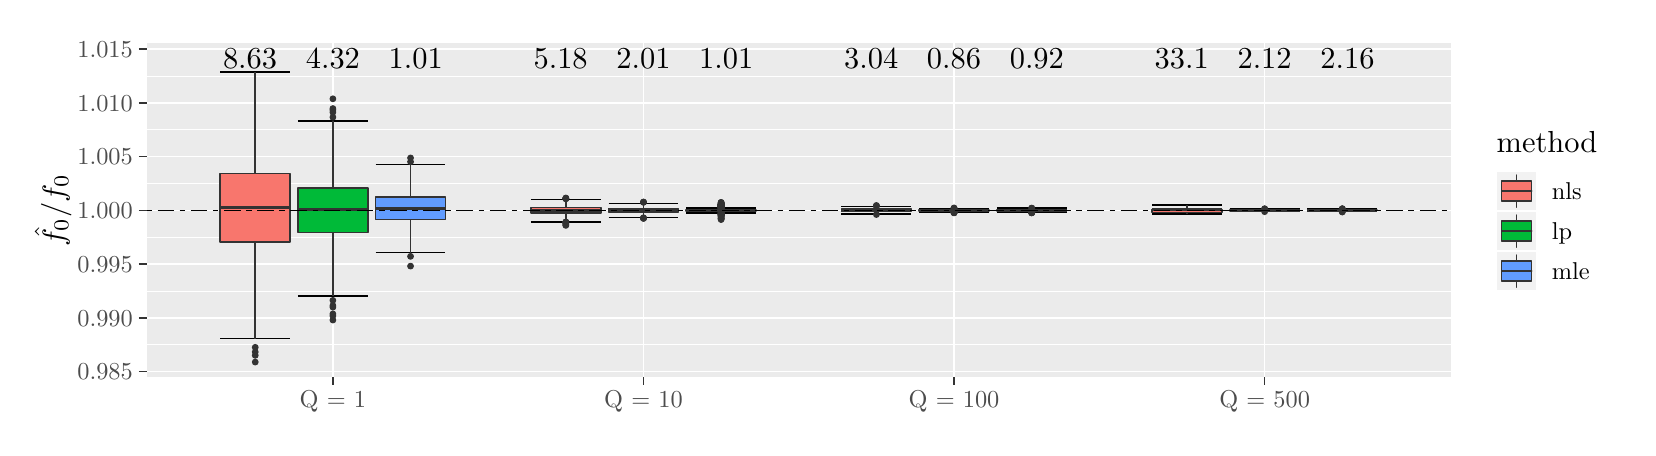
\begin{tikzpicture}[x=1pt,y=1pt]
\definecolor{fillColor}{RGB}{255,255,255}
\path[use as bounding box,fill=fillColor,fill opacity=0.00] (0,0) rectangle (578.16,144.54);
\begin{scope}
\path[clip] (  0.00,  0.00) rectangle (578.16,144.54);
\definecolor{drawColor}{RGB}{255,255,255}
\definecolor{fillColor}{RGB}{255,255,255}

\path[draw=drawColor,line width= 0.6pt,line join=round,line cap=round,fill=fillColor] (  0.00,  0.00) rectangle (578.16,144.54);
\end{scope}
\begin{scope}
\path[clip] ( 42.95, 18.22) rectangle (514.31,139.04);
\definecolor{fillColor}{gray}{0.92}

\path[fill=fillColor] ( 42.95, 18.22) rectangle (514.31,139.04);
\definecolor{drawColor}{RGB}{255,255,255}

\path[draw=drawColor,line width= 0.3pt,line join=round] ( 42.95, 29.97) --
	(514.31, 29.97);

\path[draw=drawColor,line width= 0.3pt,line join=round] ( 42.95, 49.39) --
	(514.31, 49.39);

\path[draw=drawColor,line width= 0.3pt,line join=round] ( 42.95, 68.82) --
	(514.31, 68.82);

\path[draw=drawColor,line width= 0.3pt,line join=round] ( 42.95, 88.24) --
	(514.31, 88.24);

\path[draw=drawColor,line width= 0.3pt,line join=round] ( 42.95,107.67) --
	(514.31,107.67);

\path[draw=drawColor,line width= 0.3pt,line join=round] ( 42.95,127.09) --
	(514.31,127.09);

\path[draw=drawColor,line width= 0.6pt,line join=round] ( 42.95, 20.26) --
	(514.31, 20.26);

\path[draw=drawColor,line width= 0.6pt,line join=round] ( 42.95, 39.68) --
	(514.31, 39.68);

\path[draw=drawColor,line width= 0.6pt,line join=round] ( 42.95, 59.11) --
	(514.31, 59.11);

\path[draw=drawColor,line width= 0.6pt,line join=round] ( 42.95, 78.53) --
	(514.31, 78.53);

\path[draw=drawColor,line width= 0.6pt,line join=round] ( 42.95, 97.95) --
	(514.31, 97.95);

\path[draw=drawColor,line width= 0.6pt,line join=round] ( 42.95,117.38) --
	(514.31,117.38);

\path[draw=drawColor,line width= 0.6pt,line join=round] ( 42.95,136.80) --
	(514.31,136.80);

\path[draw=drawColor,line width= 0.6pt,line join=round] (110.29, 18.22) --
	(110.29,139.04);

\path[draw=drawColor,line width= 0.6pt,line join=round] (222.52, 18.22) --
	(222.52,139.04);

\path[draw=drawColor,line width= 0.6pt,line join=round] (334.74, 18.22) --
	(334.74,139.04);

\path[draw=drawColor,line width= 0.6pt,line join=round] (446.97, 18.22) --
	(446.97,139.04);
\definecolor{drawColor}{RGB}{0,0,0}

\path[draw=drawColor,line width= 0.6pt,line join=round] ( 69.61,128.55) --
	( 94.86,128.55);

\path[draw=drawColor,line width= 0.6pt,line join=round] ( 82.23,128.55) --
	( 82.23, 32.21);

\path[draw=drawColor,line width= 0.6pt,line join=round] ( 69.61, 32.21) --
	( 94.86, 32.21);

\path[draw=drawColor,line width= 0.6pt,line join=round] ( 97.66,110.77) --
	(122.92,110.77);

\path[draw=drawColor,line width= 0.6pt,line join=round] (110.29,110.77) --
	(110.29, 47.53);

\path[draw=drawColor,line width= 0.6pt,line join=round] ( 97.66, 47.53) --
	(122.92, 47.53);

\path[draw=drawColor,line width= 0.6pt,line join=round] (125.72, 95.11) --
	(150.97, 95.11);

\path[draw=drawColor,line width= 0.6pt,line join=round] (138.35, 95.11) --
	(138.35, 63.24);

\path[draw=drawColor,line width= 0.6pt,line join=round] (125.72, 63.24) --
	(150.97, 63.24);

\path[draw=drawColor,line width= 0.6pt,line join=round] (181.83, 82.51) --
	(207.09, 82.51);

\path[draw=drawColor,line width= 0.6pt,line join=round] (194.46, 82.51) --
	(194.46, 74.39);

\path[draw=drawColor,line width= 0.6pt,line join=round] (181.83, 74.39) --
	(207.09, 74.39);

\path[draw=drawColor,line width= 0.6pt,line join=round] (209.89, 81.03) --
	(235.14, 81.03);

\path[draw=drawColor,line width= 0.6pt,line join=round] (222.52, 81.03) --
	(222.52, 75.90);

\path[draw=drawColor,line width= 0.6pt,line join=round] (209.89, 75.90) --
	(235.14, 75.90);

\path[draw=drawColor,line width= 0.6pt,line join=round] (237.95, 79.34) --
	(263.20, 79.34);

\path[draw=drawColor,line width= 0.6pt,line join=round] (250.57, 79.34) --
	(250.57, 77.68);

\path[draw=drawColor,line width= 0.6pt,line join=round] (237.95, 77.68) --
	(263.20, 77.68);

\path[draw=drawColor,line width= 0.6pt,line join=round] (294.06, 79.88) --
	(319.31, 79.88);

\path[draw=drawColor,line width= 0.6pt,line join=round] (306.69, 79.88) --
	(306.69, 77.20);

\path[draw=drawColor,line width= 0.6pt,line join=round] (294.06, 77.20) --
	(319.31, 77.20);

\path[draw=drawColor,line width= 0.6pt,line join=round] (322.12, 79.21) --
	(347.37, 79.21);

\path[draw=drawColor,line width= 0.6pt,line join=round] (334.74, 79.21) --
	(334.74, 77.85);

\path[draw=drawColor,line width= 0.6pt,line join=round] (322.12, 77.85) --
	(347.37, 77.85);

\path[draw=drawColor,line width= 0.6pt,line join=round] (350.18, 79.26) --
	(375.43, 79.26);

\path[draw=drawColor,line width= 0.6pt,line join=round] (362.80, 79.26) --
	(362.80, 77.82);

\path[draw=drawColor,line width= 0.6pt,line join=round] (350.18, 77.82) --
	(375.43, 77.82);

\path[draw=drawColor,line width= 0.6pt,line join=round] (406.29, 80.55) --
	(431.54, 80.55);

\path[draw=drawColor,line width= 0.6pt,line join=round] (418.91, 80.55) --
	(418.91, 77.19);

\path[draw=drawColor,line width= 0.6pt,line join=round] (406.29, 77.19) --
	(431.54, 77.19);

\path[draw=drawColor,line width= 0.6pt,line join=round] (434.35, 78.98) --
	(459.60, 78.98);

\path[draw=drawColor,line width= 0.6pt,line join=round] (446.97, 78.98) --
	(446.97, 78.08);

\path[draw=drawColor,line width= 0.6pt,line join=round] (434.35, 78.08) --
	(459.60, 78.08);

\path[draw=drawColor,line width= 0.6pt,line join=round] (462.40, 79.02) --
	(487.65, 79.02);

\path[draw=drawColor,line width= 0.6pt,line join=round] (475.03, 79.02) --
	(475.03, 78.06);

\path[draw=drawColor,line width= 0.6pt,line join=round] (462.40, 78.06) --
	(487.65, 78.06);
\definecolor{drawColor}{gray}{0.20}
\definecolor{fillColor}{gray}{0.20}

\path[draw=drawColor,line width= 0.4pt,line join=round,line cap=round,fill=fillColor] ( 82.23, 27.37) circle (  1.02);

\path[draw=drawColor,line width= 0.4pt,line join=round,line cap=round,fill=fillColor] ( 82.23, 23.71) circle (  1.02);

\path[draw=drawColor,line width= 0.4pt,line join=round,line cap=round,fill=fillColor] ( 82.23, 29.03) circle (  1.02);

\path[draw=drawColor,line width= 0.4pt,line join=round,line cap=round,fill=fillColor] ( 82.23, 26.14) circle (  1.02);

\path[draw=drawColor,line width= 0.6pt,line join=round] ( 82.23, 91.86) -- ( 82.23,128.55);

\path[draw=drawColor,line width= 0.6pt,line join=round] ( 82.23, 67.01) -- ( 82.23, 32.21);
\definecolor{fillColor}{RGB}{248,118,109}

\path[draw=drawColor,line width= 0.6pt,line join=round,line cap=round,fill=fillColor] ( 69.61, 91.86) --
	( 69.61, 67.01) --
	( 94.86, 67.01) --
	( 94.86, 91.86) --
	( 69.61, 91.86) --
	cycle;

\path[draw=drawColor,line width= 1.1pt,line join=round] ( 69.61, 79.61) -- ( 94.86, 79.61);
\definecolor{fillColor}{gray}{0.20}

\path[draw=drawColor,line width= 0.4pt,line join=round,line cap=round,fill=fillColor] (110.29,115.31) circle (  1.02);

\path[draw=drawColor,line width= 0.4pt,line join=round,line cap=round,fill=fillColor] (110.29, 40.40) circle (  1.02);

\path[draw=drawColor,line width= 0.4pt,line join=round,line cap=round,fill=fillColor] (110.29,114.81) circle (  1.02);

\path[draw=drawColor,line width= 0.4pt,line join=round,line cap=round,fill=fillColor] (110.29,112.18) circle (  1.02);

\path[draw=drawColor,line width= 0.4pt,line join=round,line cap=round,fill=fillColor] (110.29,118.83) circle (  1.02);

\path[draw=drawColor,line width= 0.4pt,line join=round,line cap=round,fill=fillColor] (110.29, 38.89) circle (  1.02);

\path[draw=drawColor,line width= 0.4pt,line join=round,line cap=round,fill=fillColor] (110.29, 44.13) circle (  1.02);

\path[draw=drawColor,line width= 0.4pt,line join=round,line cap=round,fill=fillColor] (110.29,113.98) circle (  1.02);

\path[draw=drawColor,line width= 0.4pt,line join=round,line cap=round,fill=fillColor] (110.29, 41.12) circle (  1.02);

\path[draw=drawColor,line width= 0.4pt,line join=round,line cap=round,fill=fillColor] (110.29, 43.54) circle (  1.02);

\path[draw=drawColor,line width= 0.4pt,line join=round,line cap=round,fill=fillColor] (110.29, 46.00) circle (  1.02);

\path[draw=drawColor,line width= 0.6pt,line join=round] (110.29, 86.64) -- (110.29,110.77);

\path[draw=drawColor,line width= 0.6pt,line join=round] (110.29, 70.51) -- (110.29, 47.53);
\definecolor{fillColor}{RGB}{0,186,56}

\path[draw=drawColor,line width= 0.6pt,line join=round,line cap=round,fill=fillColor] ( 97.66, 86.64) --
	( 97.66, 70.51) --
	(122.92, 70.51) --
	(122.92, 86.64) --
	( 97.66, 86.64) --
	cycle;

\path[draw=drawColor,line width= 1.1pt,line join=round] ( 97.66, 78.84) -- (122.92, 78.84);
\definecolor{fillColor}{gray}{0.20}

\path[draw=drawColor,line width= 0.4pt,line join=round,line cap=round,fill=fillColor] (138.35, 96.08) circle (  1.02);

\path[draw=drawColor,line width= 0.4pt,line join=round,line cap=round,fill=fillColor] (138.35, 58.38) circle (  1.02);

\path[draw=drawColor,line width= 0.4pt,line join=round,line cap=round,fill=fillColor] (138.35, 61.90) circle (  1.02);

\path[draw=drawColor,line width= 0.4pt,line join=round,line cap=round,fill=fillColor] (138.35, 97.47) circle (  1.02);

\path[draw=drawColor,line width= 0.6pt,line join=round] (138.35, 83.31) -- (138.35, 95.11);

\path[draw=drawColor,line width= 0.6pt,line join=round] (138.35, 75.22) -- (138.35, 63.24);
\definecolor{fillColor}{RGB}{97,156,255}

\path[draw=drawColor,line width= 0.6pt,line join=round,line cap=round,fill=fillColor] (125.72, 83.31) --
	(125.72, 75.22) --
	(150.97, 75.22) --
	(150.97, 83.31) --
	(125.72, 83.31) --
	cycle;

\path[draw=drawColor,line width= 1.1pt,line join=round] (125.72, 79.29) -- (150.97, 79.29);
\definecolor{fillColor}{gray}{0.20}

\path[draw=drawColor,line width= 0.4pt,line join=round,line cap=round,fill=fillColor] (194.46, 73.09) circle (  1.02);

\path[draw=drawColor,line width= 0.4pt,line join=round,line cap=round,fill=fillColor] (194.46, 74.21) circle (  1.02);

\path[draw=drawColor,line width= 0.4pt,line join=round,line cap=round,fill=fillColor] (194.46, 74.14) circle (  1.02);

\path[draw=drawColor,line width= 0.4pt,line join=round,line cap=round,fill=fillColor] (194.46, 73.29) circle (  1.02);

\path[draw=drawColor,line width= 0.4pt,line join=round,line cap=round,fill=fillColor] (194.46, 73.71) circle (  1.02);

\path[draw=drawColor,line width= 0.4pt,line join=round,line cap=round,fill=fillColor] (194.46, 74.24) circle (  1.02);

\path[draw=drawColor,line width= 0.4pt,line join=round,line cap=round,fill=fillColor] (194.46, 82.85) circle (  1.02);

\path[draw=drawColor,line width= 0.4pt,line join=round,line cap=round,fill=fillColor] (194.46, 82.99) circle (  1.02);

\path[draw=drawColor,line width= 0.4pt,line join=round,line cap=round,fill=fillColor] (194.46, 82.73) circle (  1.02);

\path[draw=drawColor,line width= 0.4pt,line join=round,line cap=round,fill=fillColor] (194.46, 74.32) circle (  1.02);

\path[draw=drawColor,line width= 0.4pt,line join=round,line cap=round,fill=fillColor] (194.46, 74.10) circle (  1.02);

\path[draw=drawColor,line width= 0.4pt,line join=round,line cap=round,fill=fillColor] (194.46, 82.77) circle (  1.02);

\path[draw=drawColor,line width= 0.4pt,line join=round,line cap=round,fill=fillColor] (194.46, 82.78) circle (  1.02);

\path[draw=drawColor,line width= 0.6pt,line join=round] (194.46, 79.56) -- (194.46, 82.51);

\path[draw=drawColor,line width= 0.6pt,line join=round] (194.46, 77.48) -- (194.46, 74.39);
\definecolor{fillColor}{RGB}{248,118,109}

\path[draw=drawColor,line width= 0.6pt,line join=round,line cap=round,fill=fillColor] (181.83, 79.56) --
	(181.83, 77.48) --
	(207.09, 77.48) --
	(207.09, 79.56) --
	(181.83, 79.56) --
	cycle;

\path[draw=drawColor,line width= 1.1pt,line join=round] (181.83, 78.38) -- (207.09, 78.38);
\definecolor{fillColor}{gray}{0.20}

\path[draw=drawColor,line width= 0.4pt,line join=round,line cap=round,fill=fillColor] (222.52, 75.63) circle (  1.02);

\path[draw=drawColor,line width= 0.4pt,line join=round,line cap=round,fill=fillColor] (222.52, 75.86) circle (  1.02);

\path[draw=drawColor,line width= 0.4pt,line join=round,line cap=round,fill=fillColor] (222.52, 81.45) circle (  1.02);

\path[draw=drawColor,line width= 0.4pt,line join=round,line cap=round,fill=fillColor] (222.52, 81.52) circle (  1.02);

\path[draw=drawColor,line width= 0.4pt,line join=round,line cap=round,fill=fillColor] (222.52, 75.72) circle (  1.02);

\path[draw=drawColor,line width= 0.4pt,line join=round,line cap=round,fill=fillColor] (222.52, 75.65) circle (  1.02);

\path[draw=drawColor,line width= 0.4pt,line join=round,line cap=round,fill=fillColor] (222.52, 81.50) circle (  1.02);

\path[draw=drawColor,line width= 0.6pt,line join=round] (222.52, 79.19) -- (222.52, 81.03);

\path[draw=drawColor,line width= 0.6pt,line join=round] (222.52, 77.86) -- (222.52, 75.90);
\definecolor{fillColor}{RGB}{0,186,56}

\path[draw=drawColor,line width= 0.6pt,line join=round,line cap=round,fill=fillColor] (209.89, 79.19) --
	(209.89, 77.86) --
	(235.14, 77.86) --
	(235.14, 79.19) --
	(209.89, 79.19) --
	cycle;

\path[draw=drawColor,line width= 1.1pt,line join=round] (209.89, 78.53) -- (235.14, 78.53);
\definecolor{fillColor}{gray}{0.20}

\path[draw=drawColor,line width= 0.4pt,line join=round,line cap=round,fill=fillColor] (250.57, 80.25) circle (  1.02);

\path[draw=drawColor,line width= 0.4pt,line join=round,line cap=round,fill=fillColor] (250.57, 79.53) circle (  1.02);

\path[draw=drawColor,line width= 0.4pt,line join=round,line cap=round,fill=fillColor] (250.57, 80.40) circle (  1.02);

\path[draw=drawColor,line width= 0.4pt,line join=round,line cap=round,fill=fillColor] (250.57, 80.35) circle (  1.02);

\path[draw=drawColor,line width= 0.4pt,line join=round,line cap=round,fill=fillColor] (250.57, 80.04) circle (  1.02);

\path[draw=drawColor,line width= 0.4pt,line join=round,line cap=round,fill=fillColor] (250.57, 79.47) circle (  1.02);

\path[draw=drawColor,line width= 0.4pt,line join=round,line cap=round,fill=fillColor] (250.57, 75.55) circle (  1.02);

\path[draw=drawColor,line width= 0.4pt,line join=round,line cap=round,fill=fillColor] (250.57, 80.05) circle (  1.02);

\path[draw=drawColor,line width= 0.4pt,line join=round,line cap=round,fill=fillColor] (250.57, 80.03) circle (  1.02);

\path[draw=drawColor,line width= 0.4pt,line join=round,line cap=round,fill=fillColor] (250.57, 80.92) circle (  1.02);

\path[draw=drawColor,line width= 0.4pt,line join=round,line cap=round,fill=fillColor] (250.57, 80.46) circle (  1.02);

\path[draw=drawColor,line width= 0.4pt,line join=round,line cap=round,fill=fillColor] (250.57, 79.65) circle (  1.02);

\path[draw=drawColor,line width= 0.4pt,line join=round,line cap=round,fill=fillColor] (250.57, 79.97) circle (  1.02);

\path[draw=drawColor,line width= 0.4pt,line join=round,line cap=round,fill=fillColor] (250.57, 75.47) circle (  1.02);

\path[draw=drawColor,line width= 0.4pt,line join=round,line cap=round,fill=fillColor] (250.57, 79.44) circle (  1.02);

\path[draw=drawColor,line width= 0.4pt,line join=round,line cap=round,fill=fillColor] (250.57, 80.35) circle (  1.02);

\path[draw=drawColor,line width= 0.4pt,line join=round,line cap=round,fill=fillColor] (250.57, 79.44) circle (  1.02);

\path[draw=drawColor,line width= 0.4pt,line join=round,line cap=round,fill=fillColor] (250.57, 80.03) circle (  1.02);

\path[draw=drawColor,line width= 0.4pt,line join=round,line cap=round,fill=fillColor] (250.57, 79.93) circle (  1.02);

\path[draw=drawColor,line width= 0.4pt,line join=round,line cap=round,fill=fillColor] (250.57, 80.00) circle (  1.02);

\path[draw=drawColor,line width= 0.4pt,line join=round,line cap=round,fill=fillColor] (250.57, 79.67) circle (  1.02);

\path[draw=drawColor,line width= 0.4pt,line join=round,line cap=round,fill=fillColor] (250.57, 77.17) circle (  1.02);

\path[draw=drawColor,line width= 0.4pt,line join=round,line cap=round,fill=fillColor] (250.57, 76.33) circle (  1.02);

\path[draw=drawColor,line width= 0.4pt,line join=round,line cap=round,fill=fillColor] (250.57, 80.50) circle (  1.02);

\path[draw=drawColor,line width= 0.4pt,line join=round,line cap=round,fill=fillColor] (250.57, 75.84) circle (  1.02);

\path[draw=drawColor,line width= 0.4pt,line join=round,line cap=round,fill=fillColor] (250.57, 79.52) circle (  1.02);

\path[draw=drawColor,line width= 0.4pt,line join=round,line cap=round,fill=fillColor] (250.57, 77.22) circle (  1.02);

\path[draw=drawColor,line width= 0.4pt,line join=round,line cap=round,fill=fillColor] (250.57, 79.81) circle (  1.02);

\path[draw=drawColor,line width= 0.4pt,line join=round,line cap=round,fill=fillColor] (250.57, 79.45) circle (  1.02);

\path[draw=drawColor,line width= 0.4pt,line join=round,line cap=round,fill=fillColor] (250.57, 80.53) circle (  1.02);

\path[draw=drawColor,line width= 0.4pt,line join=round,line cap=round,fill=fillColor] (250.57, 79.57) circle (  1.02);

\path[draw=drawColor,line width= 0.4pt,line join=round,line cap=round,fill=fillColor] (250.57, 79.38) circle (  1.02);

\path[draw=drawColor,line width= 0.4pt,line join=round,line cap=round,fill=fillColor] (250.57, 77.37) circle (  1.02);

\path[draw=drawColor,line width= 0.4pt,line join=round,line cap=round,fill=fillColor] (250.57, 80.49) circle (  1.02);

\path[draw=drawColor,line width= 0.4pt,line join=round,line cap=round,fill=fillColor] (250.57, 77.12) circle (  1.02);

\path[draw=drawColor,line width= 0.4pt,line join=round,line cap=round,fill=fillColor] (250.57, 79.65) circle (  1.02);

\path[draw=drawColor,line width= 0.4pt,line join=round,line cap=round,fill=fillColor] (250.57, 77.64) circle (  1.02);

\path[draw=drawColor,line width= 0.4pt,line join=round,line cap=round,fill=fillColor] (250.57, 80.28) circle (  1.02);

\path[draw=drawColor,line width= 0.4pt,line join=round,line cap=round,fill=fillColor] (250.57, 79.36) circle (  1.02);

\path[draw=drawColor,line width= 0.4pt,line join=round,line cap=round,fill=fillColor] (250.57, 77.65) circle (  1.02);

\path[draw=drawColor,line width= 0.4pt,line join=round,line cap=round,fill=fillColor] (250.57, 76.60) circle (  1.02);

\path[draw=drawColor,line width= 0.4pt,line join=round,line cap=round,fill=fillColor] (250.57, 80.47) circle (  1.02);

\path[draw=drawColor,line width= 0.4pt,line join=round,line cap=round,fill=fillColor] (250.57, 81.33) circle (  1.02);

\path[draw=drawColor,line width= 0.4pt,line join=round,line cap=round,fill=fillColor] (250.57, 81.38) circle (  1.02);

\path[draw=drawColor,line width= 0.4pt,line join=round,line cap=round,fill=fillColor] (250.57, 76.92) circle (  1.02);

\path[draw=drawColor,line width= 0.4pt,line join=round,line cap=round,fill=fillColor] (250.57, 79.68) circle (  1.02);

\path[draw=drawColor,line width= 0.4pt,line join=round,line cap=round,fill=fillColor] (250.57, 79.86) circle (  1.02);

\path[draw=drawColor,line width= 0.4pt,line join=round,line cap=round,fill=fillColor] (250.57, 79.57) circle (  1.02);

\path[draw=drawColor,line width= 0.4pt,line join=round,line cap=round,fill=fillColor] (250.57, 79.63) circle (  1.02);

\path[draw=drawColor,line width= 0.4pt,line join=round,line cap=round,fill=fillColor] (250.57, 80.21) circle (  1.02);

\path[draw=drawColor,line width= 0.4pt,line join=round,line cap=round,fill=fillColor] (250.57, 80.87) circle (  1.02);

\path[draw=drawColor,line width= 0.4pt,line join=round,line cap=round,fill=fillColor] (250.57, 79.53) circle (  1.02);

\path[draw=drawColor,line width= 0.4pt,line join=round,line cap=round,fill=fillColor] (250.57, 77.28) circle (  1.02);

\path[draw=drawColor,line width= 0.4pt,line join=round,line cap=round,fill=fillColor] (250.57, 79.59) circle (  1.02);

\path[draw=drawColor,line width= 0.4pt,line join=round,line cap=round,fill=fillColor] (250.57, 79.96) circle (  1.02);

\path[draw=drawColor,line width= 0.4pt,line join=round,line cap=round,fill=fillColor] (250.57, 80.21) circle (  1.02);

\path[draw=drawColor,line width= 0.4pt,line join=round,line cap=round,fill=fillColor] (250.57, 77.24) circle (  1.02);

\path[draw=drawColor,line width= 0.4pt,line join=round,line cap=round,fill=fillColor] (250.57, 79.98) circle (  1.02);

\path[draw=drawColor,line width= 0.4pt,line join=round,line cap=round,fill=fillColor] (250.57, 81.07) circle (  1.02);

\path[draw=drawColor,line width= 0.4pt,line join=round,line cap=round,fill=fillColor] (250.57, 80.10) circle (  1.02);

\path[draw=drawColor,line width= 0.4pt,line join=round,line cap=round,fill=fillColor] (250.57, 81.10) circle (  1.02);

\path[draw=drawColor,line width= 0.4pt,line join=round,line cap=round,fill=fillColor] (250.57, 79.42) circle (  1.02);

\path[draw=drawColor,line width= 0.4pt,line join=round,line cap=round,fill=fillColor] (250.57, 77.14) circle (  1.02);

\path[draw=drawColor,line width= 0.4pt,line join=round,line cap=round,fill=fillColor] (250.57, 75.56) circle (  1.02);

\path[draw=drawColor,line width= 0.4pt,line join=round,line cap=round,fill=fillColor] (250.57, 79.55) circle (  1.02);

\path[draw=drawColor,line width= 0.4pt,line join=round,line cap=round,fill=fillColor] (250.57, 79.72) circle (  1.02);

\path[draw=drawColor,line width= 0.4pt,line join=round,line cap=round,fill=fillColor] (250.57, 80.30) circle (  1.02);

\path[draw=drawColor,line width= 0.4pt,line join=round,line cap=round,fill=fillColor] (250.57, 80.50) circle (  1.02);

\path[draw=drawColor,line width= 0.4pt,line join=round,line cap=round,fill=fillColor] (250.57, 80.07) circle (  1.02);

\path[draw=drawColor,line width= 0.4pt,line join=round,line cap=round,fill=fillColor] (250.57, 79.82) circle (  1.02);

\path[draw=drawColor,line width= 0.4pt,line join=round,line cap=round,fill=fillColor] (250.57, 76.68) circle (  1.02);

\path[draw=drawColor,line width= 0.4pt,line join=round,line cap=round,fill=fillColor] (250.57, 76.42) circle (  1.02);

\path[draw=drawColor,line width= 0.4pt,line join=round,line cap=round,fill=fillColor] (250.57, 79.62) circle (  1.02);

\path[draw=drawColor,line width= 0.4pt,line join=round,line cap=round,fill=fillColor] (250.57, 80.36) circle (  1.02);

\path[draw=drawColor,line width= 0.4pt,line join=round,line cap=round,fill=fillColor] (250.57, 79.43) circle (  1.02);

\path[draw=drawColor,line width= 0.4pt,line join=round,line cap=round,fill=fillColor] (250.57, 80.09) circle (  1.02);

\path[draw=drawColor,line width= 0.4pt,line join=round,line cap=round,fill=fillColor] (250.57, 79.42) circle (  1.02);

\path[draw=drawColor,line width= 0.4pt,line join=round,line cap=round,fill=fillColor] (250.57, 80.97) circle (  1.02);

\path[draw=drawColor,line width= 0.4pt,line join=round,line cap=round,fill=fillColor] (250.57, 76.85) circle (  1.02);

\path[draw=drawColor,line width= 0.4pt,line join=round,line cap=round,fill=fillColor] (250.57, 79.79) circle (  1.02);

\path[draw=drawColor,line width= 0.4pt,line join=round,line cap=round,fill=fillColor] (250.57, 79.78) circle (  1.02);

\path[draw=drawColor,line width= 0.4pt,line join=round,line cap=round,fill=fillColor] (250.57, 79.92) circle (  1.02);

\path[draw=drawColor,line width= 0.4pt,line join=round,line cap=round,fill=fillColor] (250.57, 80.38) circle (  1.02);

\path[draw=drawColor,line width= 0.4pt,line join=round,line cap=round,fill=fillColor] (250.57, 79.72) circle (  1.02);

\path[draw=drawColor,line width= 0.4pt,line join=round,line cap=round,fill=fillColor] (250.57, 79.89) circle (  1.02);

\path[draw=drawColor,line width= 0.4pt,line join=round,line cap=round,fill=fillColor] (250.57, 79.51) circle (  1.02);

\path[draw=drawColor,line width= 0.4pt,line join=round,line cap=round,fill=fillColor] (250.57, 77.51) circle (  1.02);

\path[draw=drawColor,line width= 0.4pt,line join=round,line cap=round,fill=fillColor] (250.57, 79.69) circle (  1.02);

\path[draw=drawColor,line width= 0.4pt,line join=round,line cap=round,fill=fillColor] (250.57, 77.53) circle (  1.02);

\path[draw=drawColor,line width= 0.4pt,line join=round,line cap=round,fill=fillColor] (250.57, 79.49) circle (  1.02);

\path[draw=drawColor,line width= 0.4pt,line join=round,line cap=round,fill=fillColor] (250.57, 76.65) circle (  1.02);

\path[draw=drawColor,line width= 0.4pt,line join=round,line cap=round,fill=fillColor] (250.57, 79.53) circle (  1.02);

\path[draw=drawColor,line width= 0.4pt,line join=round,line cap=round,fill=fillColor] (250.57, 79.36) circle (  1.02);

\path[draw=drawColor,line width= 0.4pt,line join=round,line cap=round,fill=fillColor] (250.57, 77.63) circle (  1.02);

\path[draw=drawColor,line width= 0.4pt,line join=round,line cap=round,fill=fillColor] (250.57, 80.28) circle (  1.02);

\path[draw=drawColor,line width= 0.4pt,line join=round,line cap=round,fill=fillColor] (250.57, 75.96) circle (  1.02);

\path[draw=drawColor,line width= 0.4pt,line join=round,line cap=round,fill=fillColor] (250.57, 79.89) circle (  1.02);

\path[draw=drawColor,line width= 0.4pt,line join=round,line cap=round,fill=fillColor] (250.57, 79.45) circle (  1.02);

\path[draw=drawColor,line width= 0.4pt,line join=round,line cap=round,fill=fillColor] (250.57, 80.32) circle (  1.02);

\path[draw=drawColor,line width= 0.4pt,line join=round,line cap=round,fill=fillColor] (250.57, 79.36) circle (  1.02);

\path[draw=drawColor,line width= 0.4pt,line join=round,line cap=round,fill=fillColor] (250.57, 79.37) circle (  1.02);

\path[draw=drawColor,line width= 0.4pt,line join=round,line cap=round,fill=fillColor] (250.57, 80.26) circle (  1.02);

\path[draw=drawColor,line width= 0.4pt,line join=round,line cap=round,fill=fillColor] (250.57, 79.55) circle (  1.02);

\path[draw=drawColor,line width= 0.4pt,line join=round,line cap=round,fill=fillColor] (250.57, 80.70) circle (  1.02);

\path[draw=drawColor,line width= 0.4pt,line join=round,line cap=round,fill=fillColor] (250.57, 80.46) circle (  1.02);

\path[draw=drawColor,line width= 0.4pt,line join=round,line cap=round,fill=fillColor] (250.57, 79.58) circle (  1.02);

\path[draw=drawColor,line width= 0.4pt,line join=round,line cap=round,fill=fillColor] (250.57, 80.04) circle (  1.02);

\path[draw=drawColor,line width= 0.4pt,line join=round,line cap=round,fill=fillColor] (250.57, 79.38) circle (  1.02);

\path[draw=drawColor,line width= 0.4pt,line join=round,line cap=round,fill=fillColor] (250.57, 79.54) circle (  1.02);

\path[draw=drawColor,line width= 0.4pt,line join=round,line cap=round,fill=fillColor] (250.57, 76.97) circle (  1.02);

\path[draw=drawColor,line width= 0.4pt,line join=round,line cap=round,fill=fillColor] (250.57, 79.40) circle (  1.02);

\path[draw=drawColor,line width= 0.4pt,line join=round,line cap=round,fill=fillColor] (250.57, 80.27) circle (  1.02);

\path[draw=drawColor,line width= 0.4pt,line join=round,line cap=round,fill=fillColor] (250.57, 80.44) circle (  1.02);

\path[draw=drawColor,line width= 0.4pt,line join=round,line cap=round,fill=fillColor] (250.57, 80.31) circle (  1.02);

\path[draw=drawColor,line width= 0.4pt,line join=round,line cap=round,fill=fillColor] (250.57, 79.45) circle (  1.02);

\path[draw=drawColor,line width= 0.4pt,line join=round,line cap=round,fill=fillColor] (250.57, 77.10) circle (  1.02);

\path[draw=drawColor,line width= 0.4pt,line join=round,line cap=round,fill=fillColor] (250.57, 80.51) circle (  1.02);

\path[draw=drawColor,line width= 0.4pt,line join=round,line cap=round,fill=fillColor] (250.57, 80.12) circle (  1.02);

\path[draw=drawColor,line width= 0.4pt,line join=round,line cap=round,fill=fillColor] (250.57, 79.58) circle (  1.02);

\path[draw=drawColor,line width= 0.4pt,line join=round,line cap=round,fill=fillColor] (250.57, 79.50) circle (  1.02);

\path[draw=drawColor,line width= 0.4pt,line join=round,line cap=round,fill=fillColor] (250.57, 79.98) circle (  1.02);

\path[draw=drawColor,line width= 0.4pt,line join=round,line cap=round,fill=fillColor] (250.57, 79.65) circle (  1.02);

\path[draw=drawColor,line width= 0.4pt,line join=round,line cap=round,fill=fillColor] (250.57, 80.47) circle (  1.02);

\path[draw=drawColor,line width= 0.4pt,line join=round,line cap=round,fill=fillColor] (250.57, 76.93) circle (  1.02);

\path[draw=drawColor,line width= 0.4pt,line join=round,line cap=round,fill=fillColor] (250.57, 75.60) circle (  1.02);

\path[draw=drawColor,line width= 0.4pt,line join=round,line cap=round,fill=fillColor] (250.57, 79.69) circle (  1.02);

\path[draw=drawColor,line width= 0.4pt,line join=round,line cap=round,fill=fillColor] (250.57, 80.28) circle (  1.02);

\path[draw=drawColor,line width= 0.4pt,line join=round,line cap=round,fill=fillColor] (250.57, 77.65) circle (  1.02);

\path[draw=drawColor,line width= 0.4pt,line join=round,line cap=round,fill=fillColor] (250.57, 79.61) circle (  1.02);

\path[draw=drawColor,line width= 0.4pt,line join=round,line cap=round,fill=fillColor] (250.57, 79.81) circle (  1.02);

\path[draw=drawColor,line width= 0.4pt,line join=round,line cap=round,fill=fillColor] (250.57, 79.53) circle (  1.02);

\path[draw=drawColor,line width= 0.4pt,line join=round,line cap=round,fill=fillColor] (250.57, 80.24) circle (  1.02);

\path[draw=drawColor,line width= 0.4pt,line join=round,line cap=round,fill=fillColor] (250.57, 79.78) circle (  1.02);

\path[draw=drawColor,line width= 0.4pt,line join=round,line cap=round,fill=fillColor] (250.57, 79.46) circle (  1.02);

\path[draw=drawColor,line width= 0.4pt,line join=round,line cap=round,fill=fillColor] (250.57, 80.64) circle (  1.02);

\path[draw=drawColor,line width= 0.4pt,line join=round,line cap=round,fill=fillColor] (250.57, 79.67) circle (  1.02);

\path[draw=drawColor,line width= 0.4pt,line join=round,line cap=round,fill=fillColor] (250.57, 80.00) circle (  1.02);

\path[draw=drawColor,line width= 0.4pt,line join=round,line cap=round,fill=fillColor] (250.57, 76.48) circle (  1.02);

\path[draw=drawColor,line width= 0.4pt,line join=round,line cap=round,fill=fillColor] (250.57, 80.35) circle (  1.02);

\path[draw=drawColor,line width= 0.4pt,line join=round,line cap=round,fill=fillColor] (250.57, 79.55) circle (  1.02);

\path[draw=drawColor,line width= 0.4pt,line join=round,line cap=round,fill=fillColor] (250.57, 75.19) circle (  1.02);

\path[draw=drawColor,line width= 0.4pt,line join=round,line cap=round,fill=fillColor] (250.57, 80.20) circle (  1.02);

\path[draw=drawColor,line width= 0.4pt,line join=round,line cap=round,fill=fillColor] (250.57, 77.33) circle (  1.02);

\path[draw=drawColor,line width= 0.4pt,line join=round,line cap=round,fill=fillColor] (250.57, 77.63) circle (  1.02);

\path[draw=drawColor,line width= 0.4pt,line join=round,line cap=round,fill=fillColor] (250.57, 80.21) circle (  1.02);

\path[draw=drawColor,line width= 0.4pt,line join=round,line cap=round,fill=fillColor] (250.57, 79.66) circle (  1.02);

\path[draw=drawColor,line width= 0.4pt,line join=round,line cap=round,fill=fillColor] (250.57, 77.23) circle (  1.02);

\path[draw=drawColor,line width= 0.4pt,line join=round,line cap=round,fill=fillColor] (250.57, 80.40) circle (  1.02);

\path[draw=drawColor,line width= 0.4pt,line join=round,line cap=round,fill=fillColor] (250.57, 77.46) circle (  1.02);

\path[draw=drawColor,line width= 0.4pt,line join=round,line cap=round,fill=fillColor] (250.57, 77.17) circle (  1.02);

\path[draw=drawColor,line width= 0.4pt,line join=round,line cap=round,fill=fillColor] (250.57, 80.07) circle (  1.02);

\path[draw=drawColor,line width= 0.4pt,line join=round,line cap=round,fill=fillColor] (250.57, 79.53) circle (  1.02);

\path[draw=drawColor,line width= 0.4pt,line join=round,line cap=round,fill=fillColor] (250.57, 79.89) circle (  1.02);

\path[draw=drawColor,line width= 0.4pt,line join=round,line cap=round,fill=fillColor] (250.57, 79.87) circle (  1.02);

\path[draw=drawColor,line width= 0.4pt,line join=round,line cap=round,fill=fillColor] (250.57, 80.91) circle (  1.02);

\path[draw=drawColor,line width= 0.4pt,line join=round,line cap=round,fill=fillColor] (250.57, 80.58) circle (  1.02);

\path[draw=drawColor,line width= 0.4pt,line join=round,line cap=round,fill=fillColor] (250.57, 79.78) circle (  1.02);

\path[draw=drawColor,line width= 0.4pt,line join=round,line cap=round,fill=fillColor] (250.57, 79.57) circle (  1.02);

\path[draw=drawColor,line width= 0.4pt,line join=round,line cap=round,fill=fillColor] (250.57, 79.43) circle (  1.02);

\path[draw=drawColor,line width= 0.4pt,line join=round,line cap=round,fill=fillColor] (250.57, 81.34) circle (  1.02);

\path[draw=drawColor,line width= 0.6pt,line join=round] (250.57, 78.72) -- (250.57, 79.34);

\path[draw=drawColor,line width= 0.6pt,line join=round] (250.57, 78.30) -- (250.57, 77.68);
\definecolor{fillColor}{RGB}{97,156,255}

\path[draw=drawColor,line width= 0.6pt,line join=round,line cap=round,fill=fillColor] (237.95, 78.72) --
	(237.95, 78.30) --
	(263.20, 78.30) --
	(263.20, 78.72) --
	(237.95, 78.72) --
	cycle;

\path[draw=drawColor,line width= 1.1pt,line join=round] (237.95, 78.47) -- (263.20, 78.47);
\definecolor{fillColor}{gray}{0.20}

\path[draw=drawColor,line width= 0.4pt,line join=round,line cap=round,fill=fillColor] (306.69, 80.13) circle (  1.02);

\path[draw=drawColor,line width= 0.4pt,line join=round,line cap=round,fill=fillColor] (306.69, 80.29) circle (  1.02);

\path[draw=drawColor,line width= 0.4pt,line join=round,line cap=round,fill=fillColor] (306.69, 80.07) circle (  1.02);

\path[draw=drawColor,line width= 0.4pt,line join=round,line cap=round,fill=fillColor] (306.69, 77.02) circle (  1.02);

\path[draw=drawColor,line width= 0.6pt,line join=round] (306.69, 78.90) -- (306.69, 79.88);

\path[draw=drawColor,line width= 0.6pt,line join=round] (306.69, 78.21) -- (306.69, 77.20);
\definecolor{fillColor}{RGB}{248,118,109}

\path[draw=drawColor,line width= 0.6pt,line join=round,line cap=round,fill=fillColor] (294.06, 78.90) --
	(294.06, 78.21) --
	(319.31, 78.21) --
	(319.31, 78.90) --
	(294.06, 78.90) --
	cycle;

\path[draw=drawColor,line width= 1.1pt,line join=round] (294.06, 78.56) -- (319.31, 78.56);
\definecolor{fillColor}{gray}{0.20}

\path[draw=drawColor,line width= 0.4pt,line join=round,line cap=round,fill=fillColor] (334.74, 77.77) circle (  1.02);

\path[draw=drawColor,line width= 0.4pt,line join=round,line cap=round,fill=fillColor] (334.74, 77.64) circle (  1.02);

\path[draw=drawColor,line width= 0.4pt,line join=round,line cap=round,fill=fillColor] (334.74, 77.83) circle (  1.02);

\path[draw=drawColor,line width= 0.4pt,line join=round,line cap=round,fill=fillColor] (334.74, 77.76) circle (  1.02);

\path[draw=drawColor,line width= 0.4pt,line join=round,line cap=round,fill=fillColor] (334.74, 79.27) circle (  1.02);

\path[draw=drawColor,line width= 0.4pt,line join=round,line cap=round,fill=fillColor] (334.74, 77.70) circle (  1.02);

\path[draw=drawColor,line width= 0.4pt,line join=round,line cap=round,fill=fillColor] (334.74, 77.78) circle (  1.02);

\path[draw=drawColor,line width= 0.4pt,line join=round,line cap=round,fill=fillColor] (334.74, 79.33) circle (  1.02);

\path[draw=drawColor,line width= 0.4pt,line join=round,line cap=round,fill=fillColor] (334.74, 77.66) circle (  1.02);

\path[draw=drawColor,line width= 0.4pt,line join=round,line cap=round,fill=fillColor] (334.74, 79.35) circle (  1.02);

\path[draw=drawColor,line width= 0.6pt,line join=round] (334.74, 78.70) -- (334.74, 79.21);

\path[draw=drawColor,line width= 0.6pt,line join=round] (334.74, 78.35) -- (334.74, 77.85);
\definecolor{fillColor}{RGB}{0,186,56}

\path[draw=drawColor,line width= 0.6pt,line join=round,line cap=round,fill=fillColor] (322.12, 78.70) --
	(322.12, 78.35) --
	(347.37, 78.35) --
	(347.37, 78.70) --
	(322.12, 78.70) --
	cycle;

\path[draw=drawColor,line width= 1.1pt,line join=round] (322.12, 78.51) -- (347.37, 78.51);
\definecolor{fillColor}{gray}{0.20}

\path[draw=drawColor,line width= 0.4pt,line join=round,line cap=round,fill=fillColor] (362.80, 77.69) circle (  1.02);

\path[draw=drawColor,line width= 0.4pt,line join=round,line cap=round,fill=fillColor] (362.80, 77.61) circle (  1.02);

\path[draw=drawColor,line width= 0.4pt,line join=round,line cap=round,fill=fillColor] (362.80, 77.69) circle (  1.02);

\path[draw=drawColor,line width= 0.4pt,line join=round,line cap=round,fill=fillColor] (362.80, 79.34) circle (  1.02);

\path[draw=drawColor,line width= 0.4pt,line join=round,line cap=round,fill=fillColor] (362.80, 77.73) circle (  1.02);

\path[draw=drawColor,line width= 0.4pt,line join=round,line cap=round,fill=fillColor] (362.80, 77.79) circle (  1.02);

\path[draw=drawColor,line width= 0.4pt,line join=round,line cap=round,fill=fillColor] (362.80, 79.34) circle (  1.02);

\path[draw=drawColor,line width= 0.4pt,line join=round,line cap=round,fill=fillColor] (362.80, 77.66) circle (  1.02);

\path[draw=drawColor,line width= 0.6pt,line join=round] (362.80, 78.71) -- (362.80, 79.26);

\path[draw=drawColor,line width= 0.6pt,line join=round] (362.80, 78.34) -- (362.80, 77.82);
\definecolor{fillColor}{RGB}{97,156,255}

\path[draw=drawColor,line width= 0.6pt,line join=round,line cap=round,fill=fillColor] (350.18, 78.71) --
	(350.18, 78.34) --
	(375.43, 78.34) --
	(375.43, 78.71) --
	(350.18, 78.71) --
	cycle;

\path[draw=drawColor,line width= 1.1pt,line join=round] (350.18, 78.53) -- (375.43, 78.53);

\path[draw=drawColor,line width= 0.6pt,line join=round] (418.91, 78.88) -- (418.91, 80.55);

\path[draw=drawColor,line width= 0.6pt,line join=round] (418.91, 77.71) -- (418.91, 77.19);
\definecolor{fillColor}{RGB}{248,118,109}

\path[draw=drawColor,line width= 0.6pt,line join=round,line cap=round,fill=fillColor] (406.29, 78.88) --
	(406.29, 77.71) --
	(431.54, 77.71) --
	(431.54, 78.88) --
	(406.29, 78.88) --
	cycle;

\path[draw=drawColor,line width= 1.1pt,line join=round] (406.29, 78.76) -- (431.54, 78.76);
\definecolor{fillColor}{gray}{0.20}

\path[draw=drawColor,line width= 0.4pt,line join=round,line cap=round,fill=fillColor] (446.97, 79.04) circle (  1.02);

\path[draw=drawColor,line width= 0.4pt,line join=round,line cap=round,fill=fillColor] (446.97, 78.05) circle (  1.02);

\path[draw=drawColor,line width= 0.4pt,line join=round,line cap=round,fill=fillColor] (446.97, 79.03) circle (  1.02);

\path[draw=drawColor,line width= 0.4pt,line join=round,line cap=round,fill=fillColor] (446.97, 79.08) circle (  1.02);

\path[draw=drawColor,line width= 0.6pt,line join=round] (446.97, 78.65) -- (446.97, 78.98);

\path[draw=drawColor,line width= 0.6pt,line join=round] (446.97, 78.41) -- (446.97, 78.08);
\definecolor{fillColor}{RGB}{0,186,56}

\path[draw=drawColor,line width= 0.6pt,line join=round,line cap=round,fill=fillColor] (434.35, 78.65) --
	(434.35, 78.41) --
	(459.60, 78.41) --
	(459.60, 78.65) --
	(434.35, 78.65) --
	cycle;

\path[draw=drawColor,line width= 1.1pt,line join=round] (434.35, 78.54) -- (459.60, 78.54);
\definecolor{fillColor}{gray}{0.20}

\path[draw=drawColor,line width= 0.4pt,line join=round,line cap=round,fill=fillColor] (475.03, 77.94) circle (  1.02);

\path[draw=drawColor,line width= 0.4pt,line join=round,line cap=round,fill=fillColor] (475.03, 78.04) circle (  1.02);

\path[draw=drawColor,line width= 0.4pt,line join=round,line cap=round,fill=fillColor] (475.03, 79.04) circle (  1.02);

\path[draw=drawColor,line width= 0.4pt,line join=round,line cap=round,fill=fillColor] (475.03, 78.04) circle (  1.02);

\path[draw=drawColor,line width= 0.4pt,line join=round,line cap=round,fill=fillColor] (475.03, 79.08) circle (  1.02);

\path[draw=drawColor,line width= 0.4pt,line join=round,line cap=round,fill=fillColor] (475.03, 79.12) circle (  1.02);

\path[draw=drawColor,line width= 0.6pt,line join=round] (475.03, 78.66) -- (475.03, 79.02);

\path[draw=drawColor,line width= 0.6pt,line join=round] (475.03, 78.42) -- (475.03, 78.06);
\definecolor{fillColor}{RGB}{97,156,255}

\path[draw=drawColor,line width= 0.6pt,line join=round,line cap=round,fill=fillColor] (462.40, 78.66) --
	(462.40, 78.42) --
	(487.65, 78.42) --
	(487.65, 78.66) --
	(462.40, 78.66) --
	cycle;

\path[draw=drawColor,line width= 1.1pt,line join=round] (462.40, 78.54) -- (487.65, 78.54);
\definecolor{drawColor}{RGB}{0,0,0}

\path[draw=drawColor,line width= 0.6pt,dash pattern=on 2pt off 2pt on 6pt off 2pt ,line join=round] ( 42.95, 78.53) -- (514.31, 78.53);

\node[text=drawColor,anchor=base,inner sep=0pt, outer sep=0pt, scale=  1.10] at (140.22,129.75) {1.01};

\node[text=drawColor,anchor=base,inner sep=0pt, outer sep=0pt, scale=  1.10] at (110.29,129.75) {4.32};

\node[text=drawColor,anchor=base,inner sep=0pt, outer sep=0pt, scale=  1.10] at ( 80.36,129.75) {8.63};

\node[text=drawColor,anchor=base,inner sep=0pt, outer sep=0pt, scale=  1.10] at (252.44,129.75) {1.01};

\node[text=drawColor,anchor=base,inner sep=0pt, outer sep=0pt, scale=  1.10] at (222.52,129.75) {2.01};

\node[text=drawColor,anchor=base,inner sep=0pt, outer sep=0pt, scale=  1.10] at (192.59,129.75) {5.18};

\node[text=drawColor,anchor=base,inner sep=0pt, outer sep=0pt, scale=  1.10] at (364.67,129.75) {0.92};

\node[text=drawColor,anchor=base,inner sep=0pt, outer sep=0pt, scale=  1.10] at (334.74,129.75) {0.86};

\node[text=drawColor,anchor=base,inner sep=0pt, outer sep=0pt, scale=  1.10] at (304.82,129.75) {3.04};

\node[text=drawColor,anchor=base,inner sep=0pt, outer sep=0pt, scale=  1.10] at (476.90,129.75) {2.16};

\node[text=drawColor,anchor=base,inner sep=0pt, outer sep=0pt, scale=  1.10] at (446.97,129.75) {2.12};

\node[text=drawColor,anchor=base,inner sep=0pt, outer sep=0pt, scale=  1.10] at (417.04,129.75) {33.1};
\end{scope}
\begin{scope}
\path[clip] (  0.00,  0.00) rectangle (578.16,144.54);
\definecolor{drawColor}{gray}{0.30}

\node[text=drawColor,anchor=base east,inner sep=0pt, outer sep=0pt, scale=  0.88] at ( 38.00, 17.23) {0.985};

\node[text=drawColor,anchor=base east,inner sep=0pt, outer sep=0pt, scale=  0.88] at ( 38.00, 36.65) {0.990};

\node[text=drawColor,anchor=base east,inner sep=0pt, outer sep=0pt, scale=  0.88] at ( 38.00, 56.07) {0.995};

\node[text=drawColor,anchor=base east,inner sep=0pt, outer sep=0pt, scale=  0.88] at ( 38.00, 75.50) {1.000};

\node[text=drawColor,anchor=base east,inner sep=0pt, outer sep=0pt, scale=  0.88] at ( 38.00, 94.92) {1.005};

\node[text=drawColor,anchor=base east,inner sep=0pt, outer sep=0pt, scale=  0.88] at ( 38.00,114.35) {1.010};

\node[text=drawColor,anchor=base east,inner sep=0pt, outer sep=0pt, scale=  0.88] at ( 38.00,133.77) {1.015};
\end{scope}
\begin{scope}
\path[clip] (  0.00,  0.00) rectangle (578.16,144.54);
\definecolor{drawColor}{gray}{0.20}

\path[draw=drawColor,line width= 0.6pt,line join=round] ( 40.20, 20.26) --
	( 42.95, 20.26);

\path[draw=drawColor,line width= 0.6pt,line join=round] ( 40.20, 39.68) --
	( 42.95, 39.68);

\path[draw=drawColor,line width= 0.6pt,line join=round] ( 40.20, 59.11) --
	( 42.95, 59.11);

\path[draw=drawColor,line width= 0.6pt,line join=round] ( 40.20, 78.53) --
	( 42.95, 78.53);

\path[draw=drawColor,line width= 0.6pt,line join=round] ( 40.20, 97.95) --
	( 42.95, 97.95);

\path[draw=drawColor,line width= 0.6pt,line join=round] ( 40.20,117.38) --
	( 42.95,117.38);

\path[draw=drawColor,line width= 0.6pt,line join=round] ( 40.20,136.80) --
	( 42.95,136.80);
\end{scope}
\begin{scope}
\path[clip] (  0.00,  0.00) rectangle (578.16,144.54);
\definecolor{drawColor}{gray}{0.20}

\path[draw=drawColor,line width= 0.6pt,line join=round] (110.29, 15.47) --
	(110.29, 18.22);

\path[draw=drawColor,line width= 0.6pt,line join=round] (222.52, 15.47) --
	(222.52, 18.22);

\path[draw=drawColor,line width= 0.6pt,line join=round] (334.74, 15.47) --
	(334.74, 18.22);

\path[draw=drawColor,line width= 0.6pt,line join=round] (446.97, 15.47) --
	(446.97, 18.22);
\end{scope}
\begin{scope}
\path[clip] (  0.00,  0.00) rectangle (578.16,144.54);
\definecolor{drawColor}{gray}{0.30}

\node[text=drawColor,anchor=base,inner sep=0pt, outer sep=0pt, scale=  0.88] at (110.29,  7.21) {Q = 1};

\node[text=drawColor,anchor=base,inner sep=0pt, outer sep=0pt, scale=  0.88] at (222.52,  7.21) {Q = 10};

\node[text=drawColor,anchor=base,inner sep=0pt, outer sep=0pt, scale=  0.88] at (334.74,  7.21) {Q = 100};

\node[text=drawColor,anchor=base,inner sep=0pt, outer sep=0pt, scale=  0.88] at (446.97,  7.21) {Q = 500};
\end{scope}
\begin{scope}
\path[clip] (  0.00,  0.00) rectangle (578.16,144.54);
\definecolor{drawColor}{RGB}{0,0,0}

\node[text=drawColor,rotate= 90.00,anchor=base,inner sep=0pt, outer sep=0pt, scale=  1.10] at ( 13.08, 78.63) {$\hat{f_0}/f_0$};
\end{scope}
\begin{scope}
\path[clip] (  0.00,  0.00) rectangle (578.16,144.54);
\definecolor{fillColor}{RGB}{255,255,255}

\path[fill=fillColor] (525.31, 43.84) rectangle (572.66,113.42);
\end{scope}
\begin{scope}
\path[clip] (  0.00,  0.00) rectangle (578.16,144.54);
\definecolor{drawColor}{RGB}{0,0,0}

\node[text=drawColor,anchor=base west,inner sep=0pt, outer sep=0pt, scale=  1.10] at (530.81, 99.27) {method};
\end{scope}
\begin{scope}
\path[clip] (  0.00,  0.00) rectangle (578.16,144.54);
\definecolor{drawColor}{RGB}{255,255,255}
\definecolor{fillColor}{gray}{0.95}

\path[draw=drawColor,line width= 0.6pt,line join=round,line cap=round,fill=fillColor] (530.81, 78.25) rectangle (545.26, 92.70);
\end{scope}
\begin{scope}
\path[clip] (  0.00,  0.00) rectangle (578.16,144.54);
\definecolor{drawColor}{gray}{0.20}

\path[draw=drawColor,line width= 0.6pt,line join=round,line cap=round] (538.03, 79.70) --
	(538.03, 81.86);

\path[draw=drawColor,line width= 0.6pt,line join=round,line cap=round] (538.03, 89.09) --
	(538.03, 91.26);
\definecolor{fillColor}{RGB}{248,118,109}

\path[draw=drawColor,line width= 0.6pt,line join=round,line cap=round,fill=fillColor] (532.61, 81.86) rectangle (543.45, 89.09);

\path[draw=drawColor,line width= 0.6pt,line join=round,line cap=round] (532.61, 85.48) --
	(543.45, 85.48);
\end{scope}
\begin{scope}
\path[clip] (  0.00,  0.00) rectangle (578.16,144.54);
\definecolor{drawColor}{RGB}{255,255,255}
\definecolor{fillColor}{gray}{0.95}

\path[draw=drawColor,line width= 0.6pt,line join=round,line cap=round,fill=fillColor] (530.81, 63.80) rectangle (545.26, 78.25);
\end{scope}
\begin{scope}
\path[clip] (  0.00,  0.00) rectangle (578.16,144.54);
\definecolor{drawColor}{gray}{0.20}

\path[draw=drawColor,line width= 0.6pt,line join=round,line cap=round] (538.03, 65.24) --
	(538.03, 67.41);

\path[draw=drawColor,line width= 0.6pt,line join=round,line cap=round] (538.03, 74.64) --
	(538.03, 76.81);
\definecolor{fillColor}{RGB}{0,186,56}

\path[draw=drawColor,line width= 0.6pt,line join=round,line cap=round,fill=fillColor] (532.61, 67.41) rectangle (543.45, 74.64);

\path[draw=drawColor,line width= 0.6pt,line join=round,line cap=round] (532.61, 71.02) --
	(543.45, 71.02);
\end{scope}
\begin{scope}
\path[clip] (  0.00,  0.00) rectangle (578.16,144.54);
\definecolor{drawColor}{RGB}{255,255,255}
\definecolor{fillColor}{gray}{0.95}

\path[draw=drawColor,line width= 0.6pt,line join=round,line cap=round,fill=fillColor] (530.81, 49.34) rectangle (545.26, 63.80);
\end{scope}
\begin{scope}
\path[clip] (  0.00,  0.00) rectangle (578.16,144.54);
\definecolor{drawColor}{gray}{0.20}

\path[draw=drawColor,line width= 0.6pt,line join=round,line cap=round] (538.03, 50.79) --
	(538.03, 52.96);

\path[draw=drawColor,line width= 0.6pt,line join=round,line cap=round] (538.03, 60.18) --
	(538.03, 62.35);
\definecolor{fillColor}{RGB}{97,156,255}

\path[draw=drawColor,line width= 0.6pt,line join=round,line cap=round,fill=fillColor] (532.61, 52.96) rectangle (543.45, 60.18);

\path[draw=drawColor,line width= 0.6pt,line join=round,line cap=round] (532.61, 56.57) --
	(543.45, 56.57);
\end{scope}
\begin{scope}
\path[clip] (  0.00,  0.00) rectangle (578.16,144.54);
\definecolor{drawColor}{RGB}{0,0,0}

\node[text=drawColor,anchor=base west,inner sep=0pt, outer sep=0pt, scale=  0.88] at (550.76, 82.45) {nls};
\end{scope}
\begin{scope}
\path[clip] (  0.00,  0.00) rectangle (578.16,144.54);
\definecolor{drawColor}{RGB}{0,0,0}

\node[text=drawColor,anchor=base west,inner sep=0pt, outer sep=0pt, scale=  0.88] at (550.76, 67.99) {lp};
\end{scope}
\begin{scope}
\path[clip] (  0.00,  0.00) rectangle (578.16,144.54);
\definecolor{drawColor}{RGB}{0,0,0}

\node[text=drawColor,anchor=base west,inner sep=0pt, outer sep=0pt, scale=  0.88] at (550.76, 53.54) {mle};
\end{scope}
\end{tikzpicture}
}
%   \end{subfigure}
%   \caption{Comparison of two-stage NLS, LP and MLE estimators in the noise-contaminated environment. Numbers indicate MSE ratios of the corresponding estimators to the MLE at baseline.}
% \end{figure}


\end{document}
